\documentclass[5p,twocolumn]{elsarticle}

\usepackage[T1]{fontenc}
\usepackage{amsmath}
\usepackage{lipsum}
\usepackage{amssymb}
\usepackage{lineno}
\usepackage{graphicx}
\usepackage{subcaption}
\usepackage{caption}
\usepackage[utf8]{inputenc}
\usepackage[english]{babel}

\usepackage{blindtext}
\usepackage{booktabs}
\usepackage{array}
\usepackage[linesnumbered,ruled,vlined,longend]{algorithm2e}
\usepackage{mathtools}
\usepackage{pifont}
\usepackage{float}
\usepackage{ragged2e}
\usepackage{cellspace}
\usepackage{tabularx}
\newcolumntype{Z}{>{\centering\let\newline\\\arraybackslash\hspace{0pt}}X}
\renewcommand\tabularxcolumn[1]{m{#1}}
\newcolumntype{Y}{>{\raggedright\let\newline\\\arraybackslash\hspace{0pt}}X}

% Essential typography and hyphenation fixes for Elsevier format
\usepackage{microtype}  % Critical for reducing overfull boxes
\microtypesetup{protrusion=true,expansion=true}

\usepackage{xcolor, colortbl}
\usepackage{color,soul}
\usepackage{hhline}
\usepackage{makecell}
\usepackage{multirow}
\usepackage{comment}
\usepackage{xurl}
\usepackage[hidelinks, colorlinks=true]{hyperref}
\usepackage[flushleft]{threeparttable}  %%used for legend below the table
\usepackage{csquotes}
\usepackage{wasysym}

\newenvironment{highlight}{\color{red}}{}

\newenvironment{conditions*}
{\par\vspace{\abovedisplayskip}\noindent
\tabularx{\columnwidth}{>{$}l<{$} @{${}:{}$} >{\raggedright\arraybackslash}X}}
{\endtabularx\par\vspace{\belowdisplayskip}}
% define theory 

\DeclareMathOperator*{\minimize}{minimize}
% correct bad hyphenation here
\hyphenation{op-tical net-works semi-conduc-tor}


\journal{Elsevier}
\begin{document}
\begin{frontmatter}	

\title{From Trust to Augmentation: A Comprehensive Survey on Synergistic Integration of Decentralized and Generative Intelligence}

\author[add1]{Md Monjurul Karim\corref{contrib}}
\ead{karim@siat.ac.cn}
\author[add1,add2]{Sangeen Khan}
\ead{sangeenkhan2662@mails.ucas.ac.cn}
\author[add1]{Qiang Qu\corref{cor1}}
\ead{qiang@siat.ac.cn}
\author[add3]{Muhammad Muzammal}
\ead{muhammad.muzammal@northumbria.ac.uk}
\author[add4]{Kashif Sharif}
\ead{kashif@bit.edu.cn}
\author[add5]{Sujit Biswas}
\ead{sujit.biswas@city.ac.uk}

\cortext[cor1]{Corresponding Author: Qiang Qu}
\address[add1]{Shenzhen Institutes of Advanced Technology, Chinese Academy of Sciences, Shenzhen 518055, China}
\address[add2]{University of Chinese Academy of Sciences, Beijing 100049, China}
\address[add3]{Department of Computer and Information Sciences, Northumbria University, Newcastle NE7 7XA, United Kingdom}
\address[add4]{School of Computer Science and Technology, Beijing Institute of Technology, Beijing 100081, China}
\address[add5]{School of Science and Technology, City St George's, University of London, London EC1V0HB, United Kingdom}


\begin{abstract}
The integration of artificial intelligence (AI) and decentralization is reshaping application and system design across industry, government, and academia. Existing surveys typically examine blockchain, Web3, or generative models independently, which obscures the cross-layer dependencies that govern verifiability, privacy, coordination, and governance in decentralized systems. This survey bridges that gap by introducing a unified trust-to-augmentation framework that organizes the convergence into four interdependent layers: trust-based execution, privacy-preserving interoperable middleware, collaborative learning mesh, and generative augmentation. Unlike prior work that addresses these domains in isolation or in limited binary pairings, the survey explains how advances in one layer alter the requirements and surfaces of the others and identifies research gaps that arise from the integration of decentralized and generative AI. We map representative systems to the four layers and consolidate a taxonomy of enabling techniques, evaluation metrics, and layer-specific comparison tables to support consistent positioning of novel contributions. The synthesis clarifies how the convergence mitigates key limitations of centralized AI, including opacity and single points of failure. It enables automated governance, intelligent consensus, and adaptive user interfaces that preserve fault tolerance and data sovereignty. The analysis also highlights deployment challenges, including scalability bottlenecks, privacy protection under transparent ledgers, cross-chain interoperability, model interpretability, and incentive alignment. The survey identifies barriers to widespread adoption and provides strategic guidance for researchers, practitioners, and policymakers through analysis of real-world applications and deployment methodologies.
\end{abstract}

\begin{keyword}
Blockchain, Decentralized AI, Generative AI, Large Language Models, Web3
\end{keyword}

\end{frontmatter}

\section{Introduction} 
\label{sec:intro}
Intelligent systems, such as autonomous vehicles, virtual assistants, and recommendation engines, are undergoing a transformative shift from the centralized paradigm of Web2 to the emergence of decentralized Web3, which emphasizes user ownership, data privacy, and peer-to-peer interactions~\cite{yu2024toward}. While Web2 is dominated by large corporations like Google, Facebook, and Amazon, Web3 empowers users with greater control over their digital identities and establishes transparent mechanisms for data exchange~\cite{zeydan2025decentralizing}. Recent analytics indicate that the global Web3 market is anticipated to reach 33.53 billion USD by 2030, which expands at a compound annual growth rate of 49.3\% during this period\footnote{\url{https://www.grandviewresearch.com/press-release/global-web-3-0-market}}. The growth underscores Web3's potential to redefine the online ecosystem by moving away from centralized platforms and granting users control over their digital identities and assets. 

At the core of Web3's infrastructure lies blockchain, which provides the foundational framework for decentralized applications (dApps) and services. Blockchain features immutability, transparency, and security, which align seamlessly with Web3's objectives. For instance, Ethereum serves as a prominent blockchain platform that supports a wide array of decentralized applications. Ethereum's smart contract functionality facilitates the creation of dApps, decentralized finance (DeFi) platforms, and decentralized autonomous organizations (DAOs), which are pivotal in enhancing the Web3 ecosystem~\cite{hassan2025enabling}. While blockchain serves as the backbone for Web3, integrating these technologies presents challenges related to scalability, interoperability, and user experience. For example, scalability issues arise as blockchain struggles to handle large volumes of transactions without compromising performance, which is essential for Web3's broader adoption~\cite{thong2025know}. Similarly, interoperability remains a challenge due to the lack of standardized protocols across different blockchain platforms, which makes it difficult for dApps to communicate and function seamlessly~\cite{far2024third}. Furthermore, user experience can suffer because interacting with decentralized systems often requires technical knowledge, presenting a barrier to mainstream adoption~\cite{wan2024web3}. These obstacles hinder the seamless functioning of decentralized applications and services, affecting adoption and efficiency.

\subsection{Motivation and Challenges}
The convergence of AI with blockchain and Web3 technologies offers transformative opportunities for decentralized ecosystems. As these domains evolve, AI capabilities become increasingly vital for enhancing scalability, optimizing operations, and improving user experiences. However, this integration introduces several critical challenges that must be addressed. First, a fundamental centralization-decentralization conflict exists where traditional AI systems typically operate within centralized infrastructures, which directly conflicts with Web3's decentralized ethos. Current AI development relies on massive computational clusters controlled by a few major technology companies, thus contradicting blockchain's distributed consensus principles~\cite{choi2025technological}. Second, computational resource constraints severely limit integration possibilities. Modern decentralized applications require substantial resources that strain blockchain capabilities. For instance, Ethereum processes approximately 15-30 transactions per second, while complex AI operations demand billions of floating-point operations. This disparity makes on-chain AI operations prohibitively expensive and slow~\cite{feng2025efficient}. Third, privacy and data security concerns emerge when integrating AI models that require vast training datasets. This requirement creates tension with blockchain's transparent nature. When sensitive financial data from DeFi applications is used for AI training, blockchain's immutable public ledger may expose private information. This exposure can lead to compliance issues with regulations like GDPR~\cite{savadatti2025survey}. 

Generative AI (GenAI) and large models, including Large Language Models (LLMs) and Large Multimodal Models (LMMs), play an instrumental role in addressing these challenges~\cite{taylor2025examining,chang2024survey}. LLMs and LMMs are capable of understanding and generating complex content, and thereby can offer scalable and intelligent solutions for blockchain-based Web3 applications. These models can enhance data analysis, automate processes, and provide advanced interactive experiences. Integrating LLMs and LMMs into blockchain can align AI capabilities with the decentralized objectives of Web3, fostering a symbiotic relationship that enhances both fields. Despite the potential benefits, integrating GenAI with blockchain comes with significant challenges~\cite{nguyen2024generative}. One primary issue is the centralized nature of traditional AI development, which often conflicts with the decentralized framework of blockchain and Web3. On the other hand, LLM applications (e.g., ChatGPT\footnote{\url{https://chatgpt.com/}}, Gemini\footnote{\url{https://gemini.google.com/}}) require substantial computational resources, which are typically managed by centralized data centers located in the cloud~\cite{qian2024alibaba}. This centralization poses challenges in maintaining the trustless, distributed nature of Web3. Additionally, ensuring data confidentiality and security becomes complex when integrating AI models that rely on vast datasets, as blockchain's transparency can lead to concerns when AI training data or model outputs need protection. Moreover, the high computational costs associated with deploying large models on decentralized networks present another significant hurdle~\cite{chang2024survey}. These challenges underscore the need for innovative approaches to integrate these advanced AI capabilities seamlessly with blockchain and Web3.

Decentralized AI (DeAI) emerges as a solution to address some of the inherent challenges in merging AI with decentralized systems. Unlike centralized AI, DeAI operates on decentralized networks and can be aligned with the principles of blockchain and Web3~\cite{wang2024sok}. This integration allows for AI models and data to be distributed across peer-to-peer networks, and mitigates concerns related to data centralization and privacy. By distributing the training and operation of AI models across multiple nodes, it ensures that no single entity has absolute control, enhancing transparency and trust. Consequently, DeAI provides a pathway to integrate GenAI while maintaining the decentralized ethos of blockchain and Web3. By distributing model training and deployment across peer-to-peer networks, DeAI mitigates risks associated with data concentration and privacy breaches. This approach not only enhances the transparency and trust needed for blockchain and Web3 ecosystems but also optimizes the computational load by leveraging distributed resources~\cite{javadpour2024decentralized}. However, the integration of DeAI presents significant challenges, such as the need for model consistency, the prevention of malicious behavior, and the maintenance of reliable network performance, which are areas that require further exploration.

To bridge these gaps, this survey adopts a structural approach that moves beyond isolated technology analysis. We address the identified conflicts between centralization and decentralization by proposing a unified architecture that layers trust-based execution, privacy-preserving middleware, and collaborative learning meshes beneath generative augmentation. This hierarchical organization allows us to map the technical bottlenecks identified above, such as computational scalability and data confidentiality, to distinct architectural solutions. It also establishes the rationale for the comprehensive framework detailed in the subsequent sections.


\subsection{Existing Surveys}
Intelligent systems present transformative opportunities for building secure, transparent, and scalable digital ecosystems that align with user-centric and decentralized principles. This integration is essential to address limitations in traditional centralized systems, including data privacy, operational inefficiencies, and lack of interoperability. However, existing surveys primarily examine only specific pairs of these topics, which results in a critical gap in understanding the broader impact of their combined potential. Current research in this area is mainly categorized into three themes: (i) Blockchain and LLMs, (ii) Blockchain, Web3, and DeAI, and (iii) Security and Privacy aspects of GenAI. This paper uniquely addresses this gap by offering a comprehensive analysis of these technologies' intersections and provides insights into how their integration can enhance scalability, security, and interoperability for next-generation decentralized applications. Table~\ref{tab:related} provides a detailed comparison between existing surveys and our work.

\begin{table*}[!t]
\centering
\caption{Comparison of existing studies and our survey.}
\label{tab:related}
\footnotesize
\begin{tabularx}{\linewidth}{>{\hsize=0.06\hsize}Z>{\hsize=0.09\hsize}Z>{\hsize=0.05\hsize}Z>{\hsize=0.05\hsize}Z>{\hsize=0.06\hsize}Z>{\hsize=0.05\hsize}Z>{\hsize=0.50\hsize}X} 
\toprule

\textbf{Ref.} & \makecell[c]{\textbf{Blockchain}} & \makecell[c]{\textbf{Web3}} & \makecell[c]{\textbf{DeAI}} & \makecell[c]{\textbf{GenAI}} & \makecell[c]{\textbf{LLMs}} & \makecell[c]{\textbf{Remarks}} \\\toprule 

\cite{he2024large} & \ding{51} & \ding{53} & \ding{53} & \ding{53} & \ding{51} & Analyze LLM applications in improving blockchain security and threat detection \\

\cite{geren2025blockchain} & \ding{51} & \ding{53} & \ding{53} & \ding{53} & \ding{51} & Review blockchain's role in enhancing security and decentralization for LLMs \\

\cite{luo2024bc4llm} & \ding{51} & \ding{51} & \ding{53} & \ding{53} & \ding{51} & Examine blockchain's role in increasing trust and transparency in \newline AI-generated content \\\midrule

\cite{cao2022decentralized} & \ding{51} & \ding{51} & \ding{51} & \ding{53} & \ding{53} & Investigate DeAI's contributions to blockchain and metaverse \newline integration \\

\cite{kersic2024review} & \ding{51} & \ding{51} & \ding{51} & \ding{53} & \ding{53} & Review foundational components necessary for building DeAI systems \\

\cite{li2024blockchain} & \ding{51} & \ding{51} & \ding{53} & \ding{51} & \ding{53} & Explore the integration of AI into intelligent blockchain systems for Web3 \\

\cite{ressi2024ai} & \ding{51} & \ding{51} & \ding{53} & \ding{51} & \ding{53} & Review AI-driven enhancements to blockchain efficiency and security \\

\cite{saleh2024blockchain} & \ding{51} & \ding{51} & \ding{51} & \ding{53} & \ding{53} & Examine the integration of blockchain and decentralized AI for \newline cybersecurity \\

\cite{shen2024artificial} & \ding{51} & \ding{51} & \ding{51} & \ding{51} & \ding{53} & Analyze AI's role in solving challenges within Web3 architecture \\

\cite{zhu2024survey} & \ding{51} & \ding{51} & \ding{51} & \ding{51} & \ding{53} & Survey blockchain, AI, and edge computing technologies for Web3 development \\\midrule

\cite{friha2024llm} & \ding{53} & \ding{53} & \ding{51} & \ding{51} & \ding{51} & Review LLM-based edge intelligence architectures, applications, and security concerns \\

\cite{golda2024privacy} & \ding{53} & \ding{53} & \ding{53} & \ding{51} & \ding{51} & Investigate privacy and security concerns in generative AI systems \\

\cite{kheddar2024transformers} & \ding{53} & \ding{53} & \ding{53} & \ding{51} & \ding{51} & Review the use of Transformers and LLMs in improving intrusion detection systems \\

\cite{hagos2024recent} & \ding{53} & \ding{53} & \ding{53} & \ding{51} & \ding{51} & Explore advancements and challenges of generative AI and LLMs in NLP \\\midrule

\textbf{Our Survey} & \ding{51} & \ding{51} & \ding{51} & \ding{51} & \ding{51} & Inquire blockchain, Web3, DeAI, GenAI, LLMs and beyond for \newline security, scalability, and interoperability \\\bottomrule

\end{tabularx}
\end{table*}

\subsubsection{Integration of Blockchain and LLMs}
Surveys in~\cite{he2024large, geren2025blockchain, luo2024bc4llm} focus on leveraging blockchain's inherent data integrity and transparency features to enhance the trustworthiness of LLM applications. For example, He et al.~\cite{he2024large} explore the integration of blockchain-driven data integrity with the generative capabilities of LLMs to emphasize trust, transparency, and enhancement of privacy-preserving applications. They identify key domains such as healthcare and finance, where blockchain can provide reliable data verification for LLM outputs while mitigating risks related to data quality and biases. Similarly, Geren et al.~\cite{geren2025blockchain} highlight the decentralized approach as a means to ensure data transparency while preventing single points of failure in LLM deployments. They particularly underscore the use of blockchain for maintaining audit trails of AI model interactions, which contributes to improved accountability and robustness against adversarial activities such as prompt injection attacks, hallucinations, data poisoning, and inference attacks. Furthermore, Luo et al.~\cite{luo2024bc4llm} underline the challenges such as scalability, storage overhead, energy consumption, heterogeneity, and interpretability.

\subsubsection{Integration of Blockchain, Web3, and DeAI}
DeAI combined with blockchain and Web3 presents unique opportunities to improve scalability, privacy, and decentralized decision-making, making it a key area of focus for recent research~\cite{cao2022decentralized,kersic2024review,li2024blockchain,ressi2024ai,saleh2024blockchain,shen2024artificial,zhu2024survey}. For example, Cao et al.~\cite{cao2022decentralized} highlight use cases where blockchain-driven data integrity mechanisms ensure trust in Web3 environments, including applications in decentralized finance (DeFi) and autonomous data marketplaces. Likewise, Kersic et al.~\cite{kersic2024review} explore the roles of edge computing and blockchain in reducing latency and improving the security of DeAI services in the context of Web3. Consequently, Li et al.~\cite{li2024blockchain} provide an analysis of different blockchain-based consensus mechanisms to evaluate their suitability for managing data generated by DeAI models. Similarly, Ressi et al.~\cite{ressi2024ai} propose a taxonomy for categorizing AI-enabled blockchain applications and discuss how these integrations can provide adaptive and intelligent consensus mechanisms, thereby increasing system resilience against adversarial threats. Additionally, Saleh et al.~\cite{saleh2024blockchain} provide a comprehensive taxonomy of cybersecurity challenges in the integration of blockchain and DeAI. On the other hand, Shen et al.~\cite{shen2024artificial} suggest leveraging cross-chain interoperability and decentralized storage solutions to create more cohesive Web3 ecosystems. They particularly emphasize the role of DeAI in enhancing the adaptability of blockchain to Web3 dynamics. Furthermore, Zhu et al.~\cite{zhu2024survey} emphasize the benefits of integrated blockchain, AI, edge computing, and Web3 solutions to address the challenges in decentralization, data ownership, privacy, and security.

\subsubsection{Security and Privacy Aspects of GenAI}
As for the generic security and privacy aspects of GenAI, recent surveys~\cite{friha2024llm,golda2024privacy,kheddar2024transformers,hagos2024recent} have explored the challenges and potential solutions to address vulnerabilities and ensure responsible deployment. For instance, Friha et al.~\cite{friha2024llm} explore security vulnerabilities that arise in deploying LLMs in edge computing environments. The authors identify specific attack vectors (e.g., data breaches, model tampering), and suggest defense mechanisms such as adversarial training, differential privacy, federated learning (FL), model quantization, pruning, and encryption to mitigate these risks. Besides, Golda et al.~\cite{golda2024privacy} emphasize privacy and security concerns (e.g., adversarial attacks, deepfake, data breaches) of GenAI and outline a detailed roadmap for ethical deployment in the form of data governance policies and interdisciplinary collaboration between developers and regulators. Moreover, Kheddar et al.~\cite{kheddar2024transformers} investigate the application of Transformer and LLMs for enhancing Intrusion Detection Systems (IDS) and discuss the challenges such as high computational requirements and lack of interpretability. Furthermore, Hagos et al.~\cite{hagos2024recent} provide a holistic review of GenAI and LLMs to highlight their transformative potential across various domains, including natural language processing (NLP), image generation, and code completion.


	
\subsubsection{Comparison with Existing Surveys}
Building on the comparison in Table~\ref{tab:related}, the main novelty of this survey is that it does not treat these themes as separate tracks. Instead, it studies their convergence as a single decentralized intelligence problem and explains how advances in one pillar reshape the design space of the others. Surveys on blockchain and LLMs primarily emphasize trust and auditability for large models~\cite{he2024large,geren2025blockchain,luo2024bc4llm}. In parallel, surveys on blockchain, Web3, and DeAI concentrate on distributed learning infrastructures and system architectures~\cite{cao2022decentralized,kersic2024review,li2024blockchain,ressi2024ai,saleh2024blockchain,shen2024artificial,zhu2024survey}. On the other hand, GenAI security surveys focus on model-level risks and defences~\cite{friha2024llm,golda2024privacy,kheddar2024transformers,hagos2024recent}. None of these works explains how trust-based execution, privacy-preserving interoperability, collaborative learning meshes, and generative augmentation must be co-designed to deliver decentralized intelligence end to end. Our trust-to-augmentation framework fills this gap by unifying all five pillars into four interacting layers and enabling a cross-layer view of architectures, incentives, governance, and deployments that is absent from prior surveys.





\subsection{Research Methodology}
This section outlines the systematic methodology used to structure the literature review on converging decentralized and intelligent systems. The methodology follows established principles inspired by the Preferred Reporting Items for Systematic Reviews and Meta-Analyses (PRISMA) guidelines~\cite{page2021prisma}. Transparent and reproducible selection criteria are applied to address clearly defined research questions while preserving high relevance and methodological rigor. Figure~\ref{fig:method} illustrates the overall literature search and study selection process.

\begin{figure}[!t]
\centering
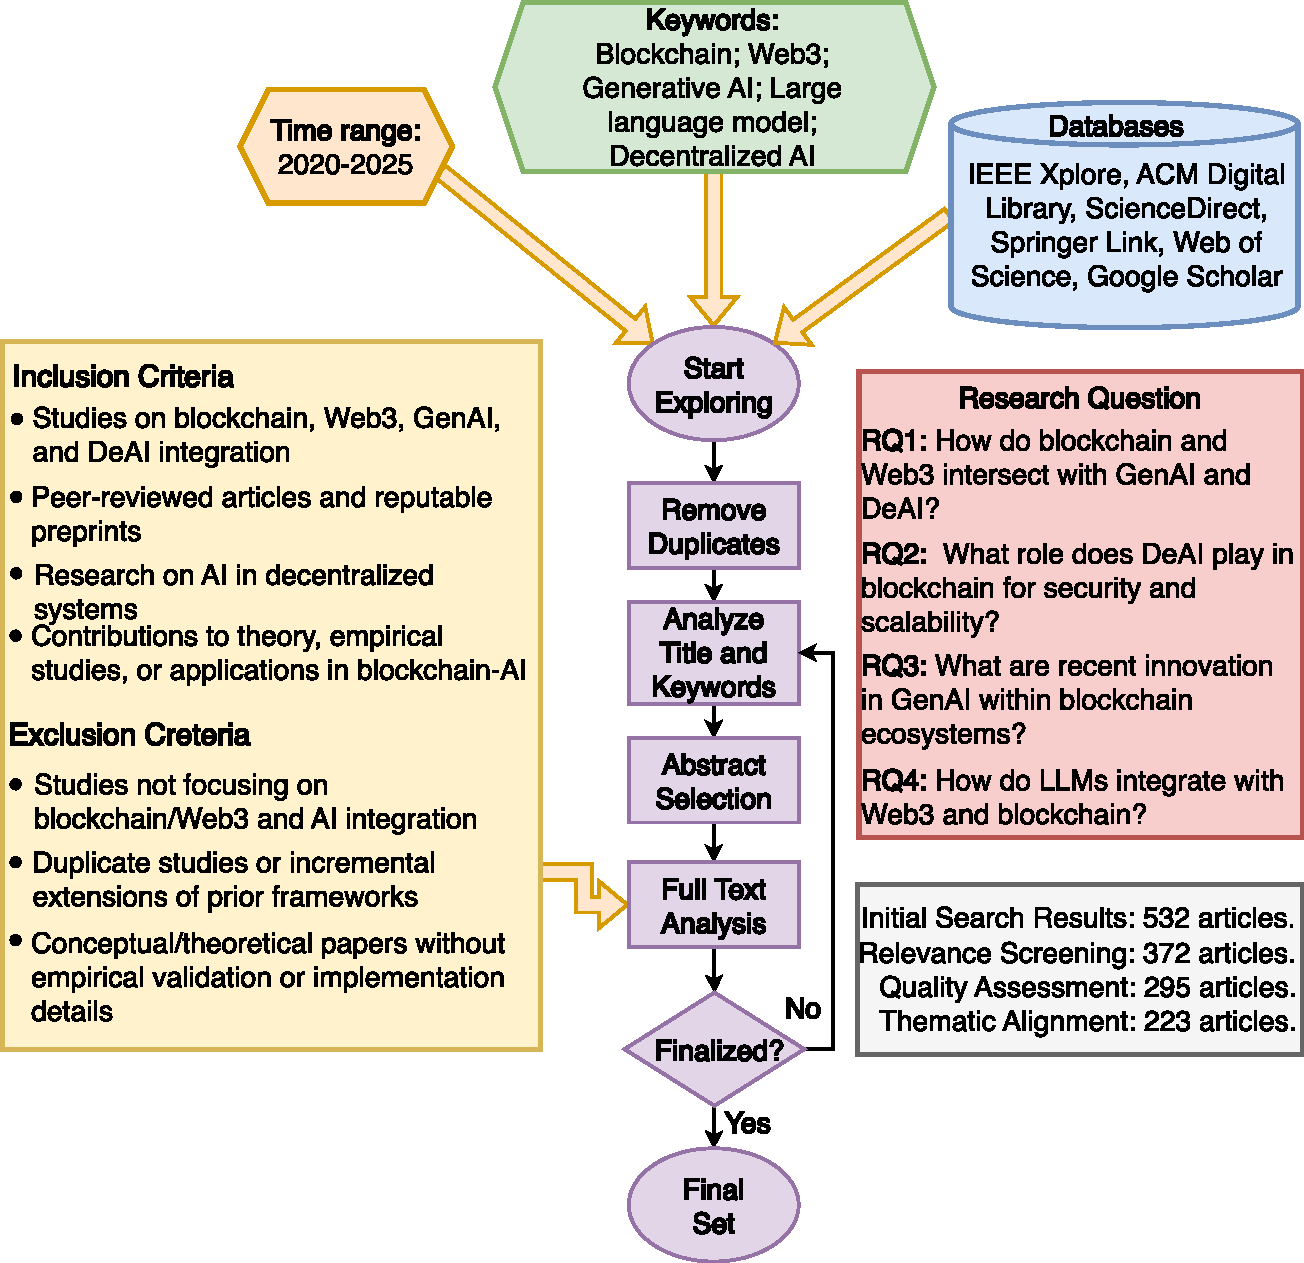
\includegraphics[width=\linewidth]{method.pdf}
\caption{Systematic representation of the literature search and selection process. }
\label{fig:method}
\end{figure}

\textbf{Search Strategy and Corpus:}
Our literature search was conducted across six major scholarly databases (IEEE Xplore, ACM Digital Library, ScienceDirect, SpringerLink, Web of Science, and Google Scholar) covering the period 2020--2025, a critical timeframe for blockchain-AI integration advancements. Keywords targeting blockchain, Web3, DeAI, GenAI, and LLMs were systematically combined using Boolean logic to ensure comprehensive retrieval. Search queries were adapted to each database interface, and the reference lists of key surveys and highly cited studies were inspected to identify additional relevant works. As shown in the corpus analysis in Figure~\ref{fig:analytical}, the word-cloud visualization reveals dominant research themes including \emph{Decentralized AI} and \emph{Generative AI}, while the year-wise distribution confirms the contemporary relevance of the scope, with nearly half of the studies published in 2024.

\textbf{Screening and Quality Assessment:}
The initial search identified 532 candidate publications. We employed a multi-stage screening procedure: duplicate removal and title/abstract screening reduced the set to 372 articles, and full-text assessment refined the set to 223 selected studies. Beyond the mechanical application of PRISMA steps, we assessed each candidate paper along three dimensions to ensure quality: (1) \textit{Topical Alignment} required studies to address the convergence of at least two pillars (e.g., blockchain and GenAI) rather than mentioning them as background; (2) \textit{Integration Focus} emphasized contributions to architectures, protocols, or workflows that span multiple pillars; and (3) \textit{Methodological Robustness} ensured the selection of peer-reviewed articles, admitting preprints only if they provided comprehensive system descriptions, rigorous empirical evaluations, or verifiable open-source artifacts. Conceptual position papers without concrete mechanisms and incremental extensions of earlier work were excluded.

 \begin{figure*}[!t]
	\centering
	\begin{subfigure}[b]{0.45\linewidth}
		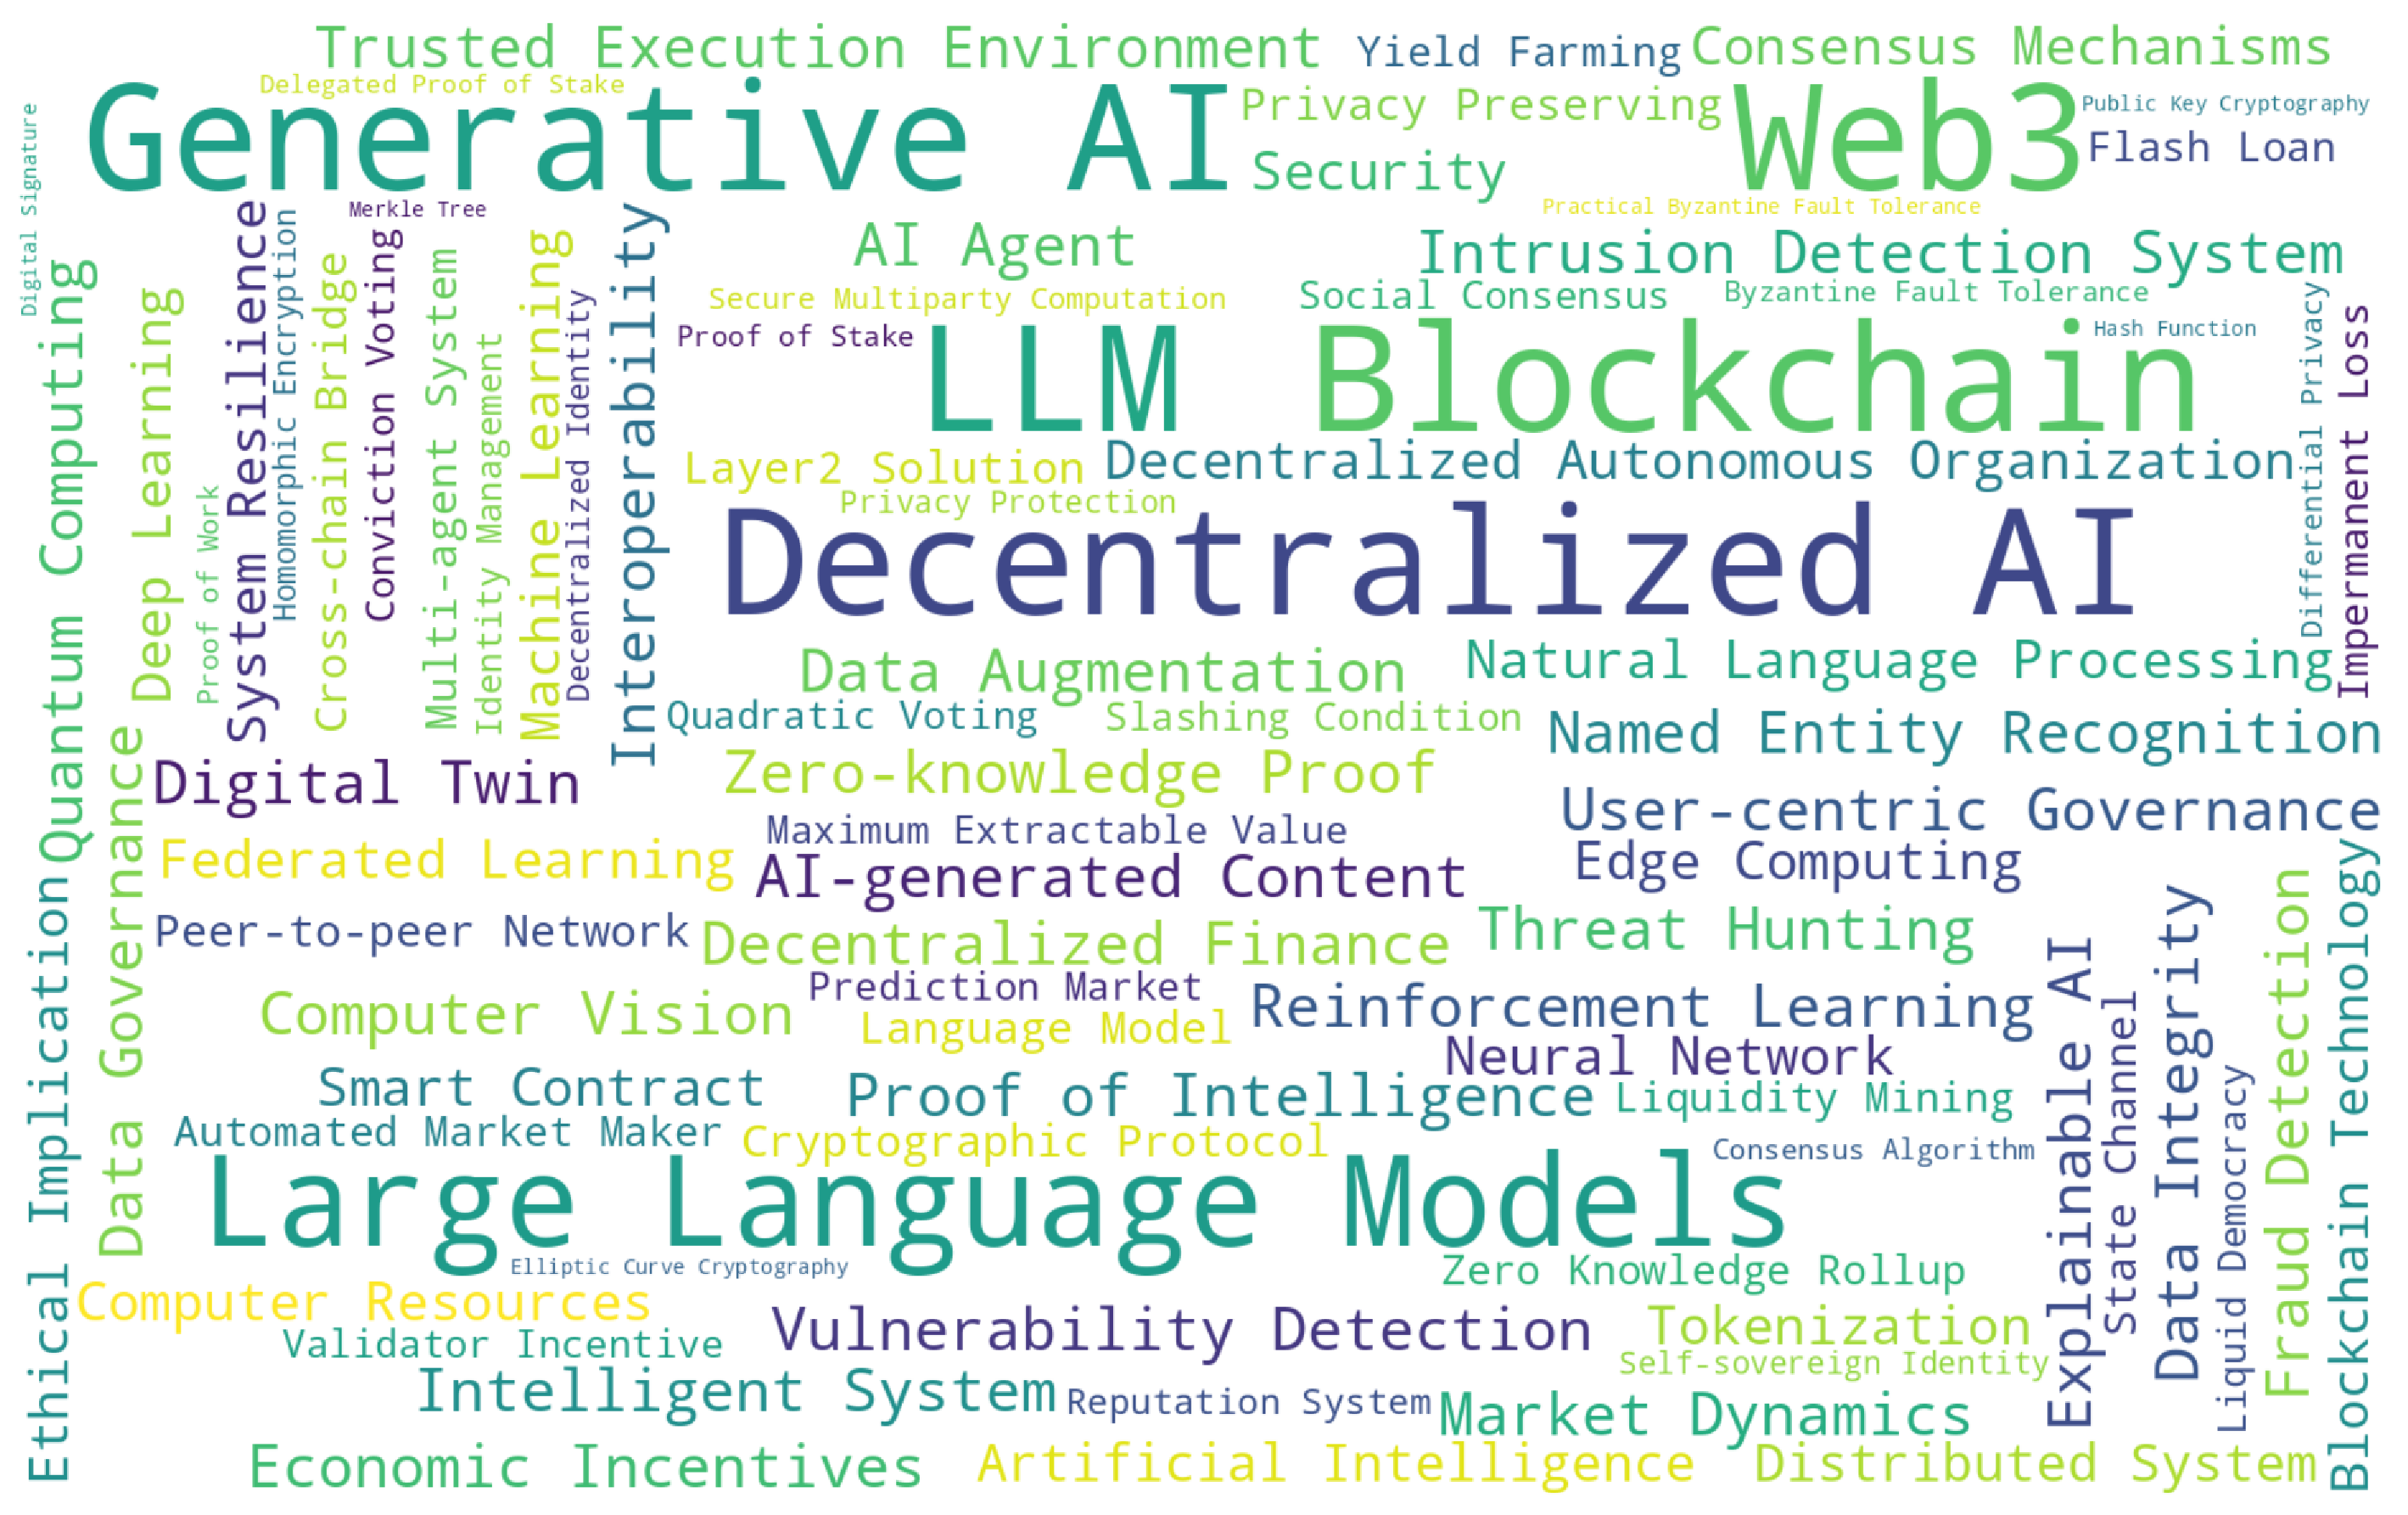
\includegraphics[width=\textwidth]{wordcloud.pdf}
		\caption{Word-cloud of high-frequency terms.}
		\label{fig:wordcloud}
	\end{subfigure}
	\begin{subfigure}[b]{0.45\linewidth}
		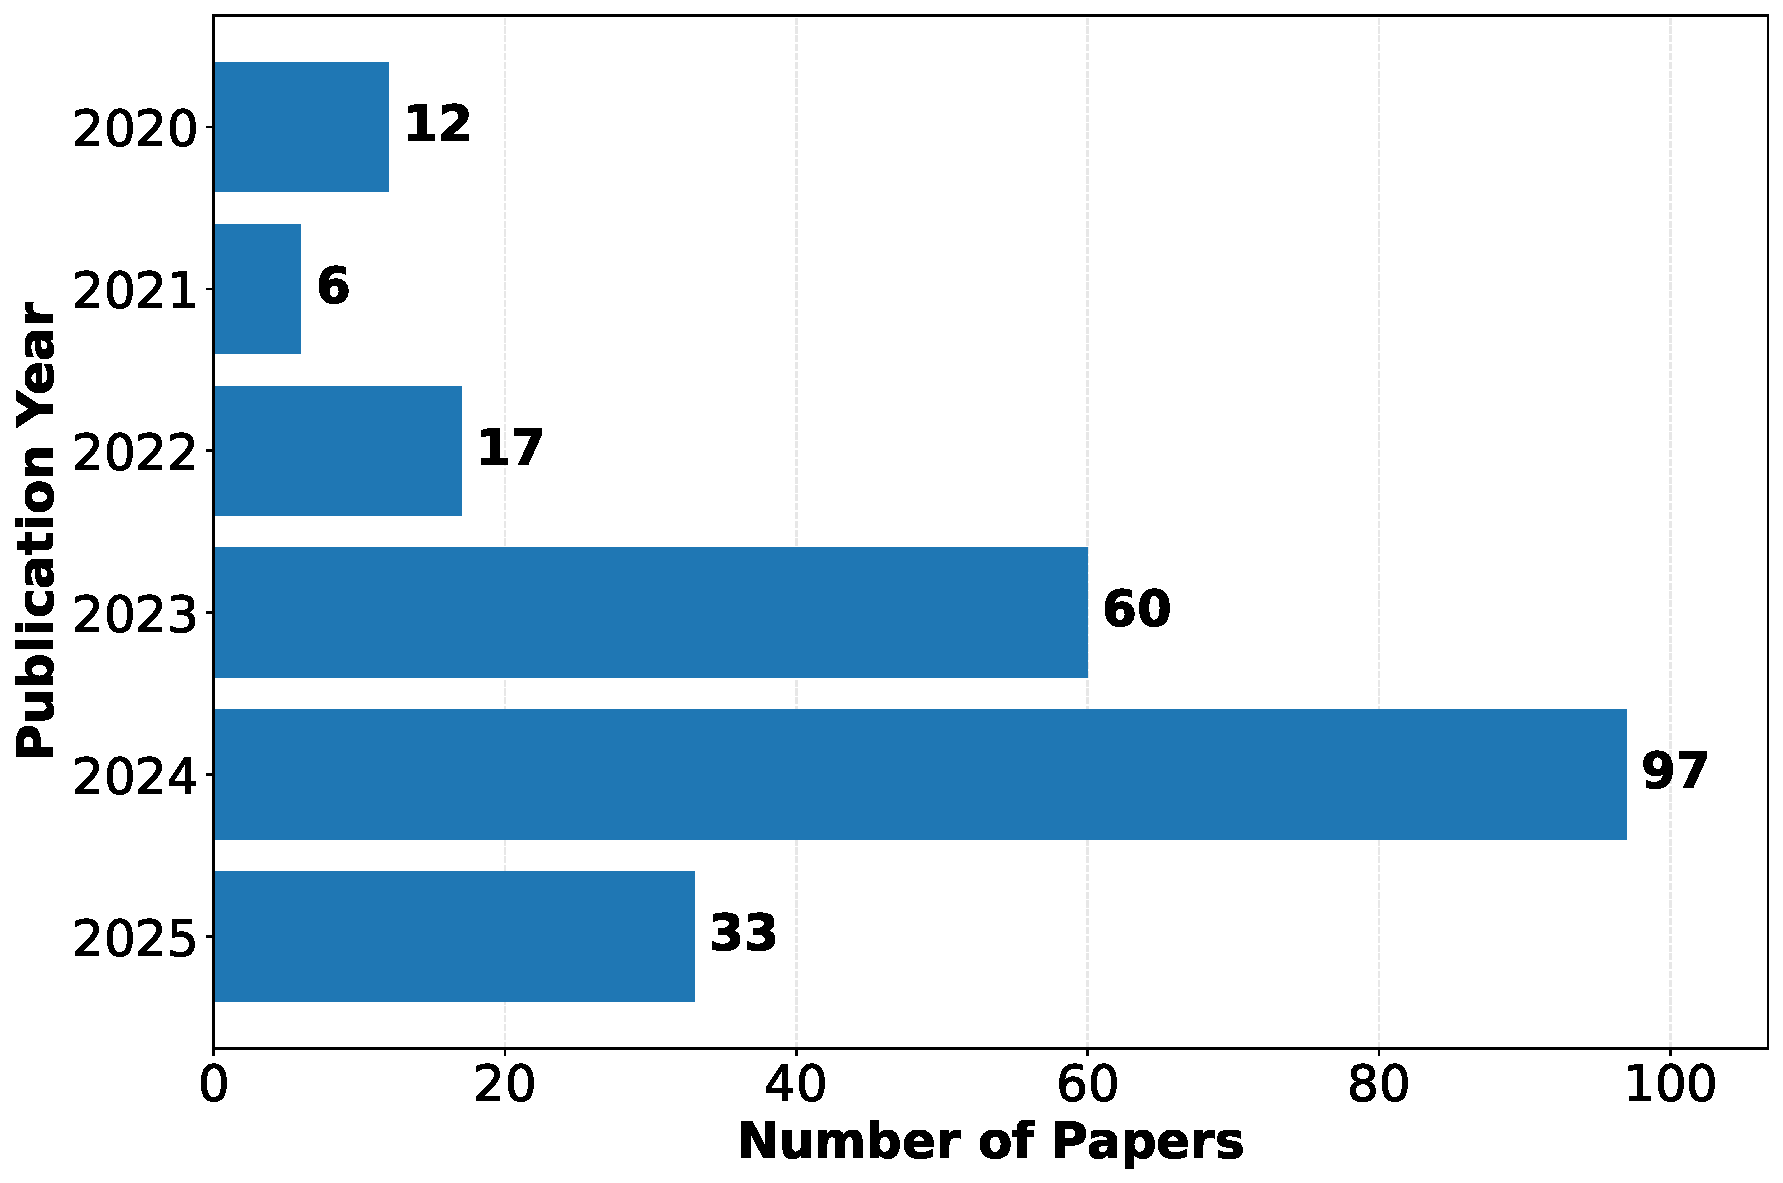
\includegraphics[width=\textwidth]{distribution.pdf}
		\caption{Distribution of studies by publication year.}
		\label{fig:distribution}
	\end{subfigure}
	\caption{Literature corpus analysis and publication trends.}
	\label{fig:analytical}
\end{figure*}

\textbf{Quantitative Synthesis and Categorization:}
We complement the qualitative review with a structured quantitative synthesis to organize the selected corpus. First, we manually assigned each paper to topic categories such as \textquote{blockchain and LLMs} or \textquote{GenAI security} based on abstract and keyword analysis. These categories align with the four layers of our trust-to-augmentation framework and support the taxonomy developed in later sections. Second, we computed term frequencies to verify that these categories capture the main research themes. Finally, for central works in each category, we inspected citation and co-citation information to identify clusters of closely related studies. This step guided the selection of representative systems and reduced the risk of over-representing multiple papers that report essentially the same architecture or dataset.




\subsection{Contribution and Organization of this Survey}
Despite the notable contributions made by existing works on blockchain, LLMs, Web3, DeAI, and GenAI, there are several limitations that need to be addressed. The blockchain and LLM-based studies~\cite{he2024large,geren2025blockchain,luo2024bc4llm} do not discuss the scalability and interoperability challenges when integrating blockchain and LLMs in large-scale environments. On the other hand, studies~\cite{cao2022decentralized,kersic2024review,li2024blockchain,ressi2024ai,saleh2024blockchain,shen2024artificial,zhu2024survey} focus heavily on theoretical frameworks without providing sufficient practical validation or real-world implementation, which limits the practical applicability of blockchain and Web3~\cite{hui2025decentralization}. Although studies~\cite{friha2024llm,golda2024privacy,kheddar2024transformers,hagos2024recent} identify the security and privacy challenges of GenAI, they overlook the depth required for deployment with other innovations, which remain exploratory rather than practical. 

To address these limitations, we focus on identifying key challenges and opportunities for improving scalability, interoperability, and application within decentralized environments. We explore the extended capabilities of blockchain, specifically in the context of intelligent consensus mechanisms and decentralized infrastructures. For example, we investigate how Proof of Intelligence (PoI) and Proof of AI-Generated Content (AIGC) can be used to validate AI-generated outputs and incentivize valuable contributions within decentralized networks. Consequently, we explore scalability and interoperability enhancements such as Layer-2 (L2) solutions (e.g., Polygon and Optimism) and protocols (e.g., Cosmos~\cite{kwon2019cosmos}, Polkadot~\cite{wood2016polkadot}) in terms of seamless cross-chain communication and integration. These methods are crucial for addressing efficiency challenges when integrating blockchain with AI models and Web3 applications. Unlike previous works, we highlight the importance of assessing practical implications by providing detailed insights into existing implementations and their applicability in real-world use cases. Additionally, we focus on concrete security measures, including privacy-preserving techniques like secure multi-party computation (SMPC)~\cite{du2001secure} and zero-knowledge proofs (ZKPs), which enhance both security and ethical compliance in decentralized systems. Furthermore, we provide a roadmap based on an interdisciplinary approach to create a secure, transparent, and ethical AI landscape. To the best of our knowledge, this survey is the first to provide an integrated view of blockchain, Web3, DeAI, and GenAI with a focus on their synergistic potential in addressing their combined challenges and opportunities. The systematic representation of the literature search and selection process is shown in Figure~\ref{fig:method}.

The primary contributions of this survey are as follows:
\begin{itemize}

\item Establishes a unified trust-to-augmentation framework that systematically organizes blockchain, Web3, DeAI, and GenAI into four synergistic layers, revealing how these technologies build upon each other to enable decentralized intelligence.
  
\item Identifies novel architectural patterns including intelligent consensus mechanisms, privacy-preserving middleware protocols, and collaborative learning infrastructures that bridge the gap between centralized AI capabilities and decentralized system requirements.
  
\item Demonstrates how the convergence of these technologies creates new security paradigms, trust mechanisms, and governance models that transcend the limitations of individual technology domains.
  
\item Provides comprehensive analysis of real-world implementations across finance, healthcare, and governance domains, revealing both the transformative potential and practical deployment challenges of decentralized intelligence systems.
  
\item Delivers a strategic research roadmap with concrete implementation timelines and actionable guidance for overcoming scalability, interpretability, and ethical deployment challenges in next-generation decentralized intelligent systems.

\end{itemize}

The remainder of this paper is organized as follows: Section~\ref{sec:back} provides the background, presenting foundational concepts necessary to understand these technologies and their interplay. Section~\ref{sec:framework} introduces a unified framework, establishing the four-layer architecture that organizes blockchain, Web3, DeAI, and GenAI into synergistic components for decentralized intelligence systems. Section~\ref{sec:blockchain} examines trust-based execution mechanisms that establish programmable infrastructure and intelligent consensus for decentralized intelligence. Section~\ref{sec:web3} explores privacy-preserving interoperable middleware that enables secure cross-chain communication and user-centric governance. Section~\ref{sec:deai} analyzes collaborative learning mesh architectures that facilitate distributed AI coordination and secure workflow management. Section~\ref{sec:genai} investigates generative augmentation capabilities that enhance user-centric governance through automated security analysis and adaptive interfaces. Section~\ref{sec:app} presents practical applications and real-world use cases demonstrating the framework's implementation across various domains, while Section~\ref{sec:future} identifies key challenges and future research directions for advancing decentralized intelligence systems. Finally, Section~\ref{sec:end} concludes with a comprehensive summary of key findings and strategic implications for the field.

\begin{figure*}[!t]
\centering
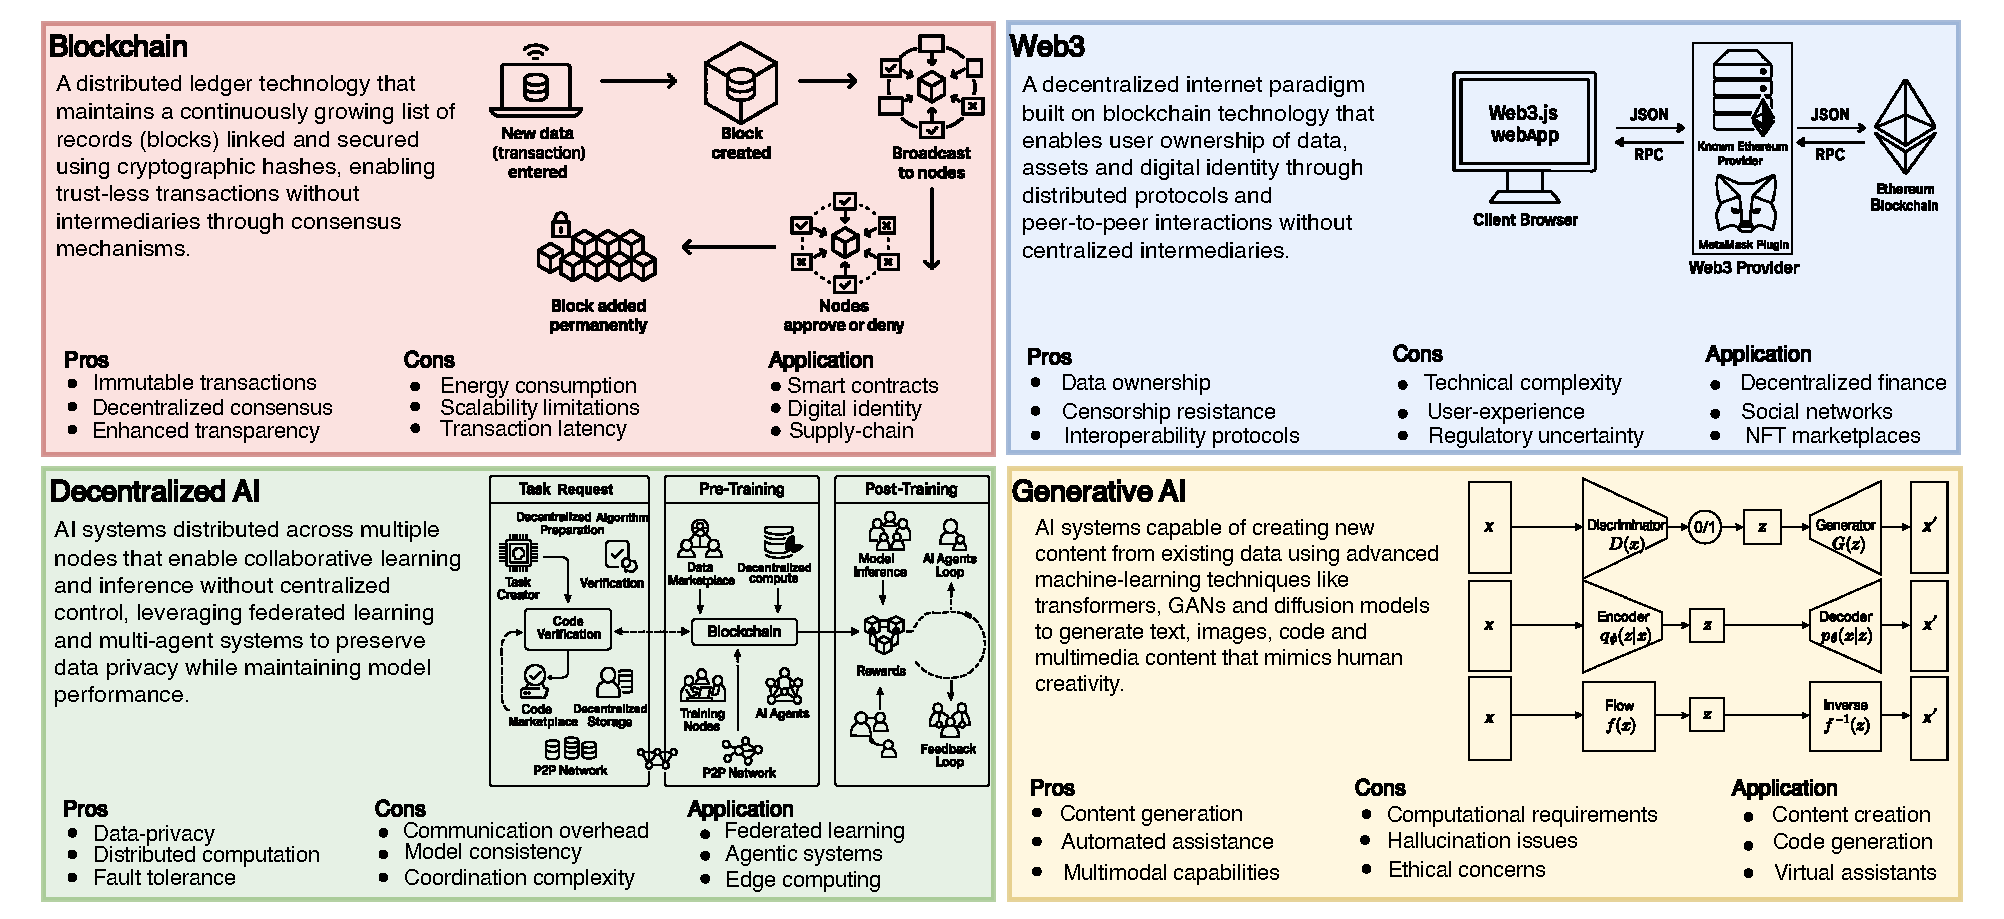
\includegraphics[width=\linewidth]{overview.pdf}
\caption{Brief overview of foundational concepts.}
\label{fig:overview}
\end{figure*}


\section{Foundational Knowledge} \label{sec:back}
In this section, we provide a foundational overview of blockchain, Web3, DeAI, GenAI, and large models. In essence, we focus on their foundational insights to create a comprehensive outline for understanding the advanced and interconnected solutions illustrated throughout this survey. A brief overview of these technologies is shown in Fig. \ref{fig:overview}.

\subsection{Blockchain}
Blockchain is a distributed ledger technology that records transactions between parties in a decentralized, verifiable, and permanent manner~\cite{xu2024survey,qu2019spatio,muzammal2019renovating}. Transactions are grouped into blocks, and blocks are cryptographically linked using hash pointers. Major blockchain platforms such as Bitcoin~\cite{karim2025bitcoin} and Ethereum validate and secure new blocks through consensus protocols, including Proof-of-Work (PoW) and Proof-of-Stake (PoS). These networks rely on cryptoeconomic incentives, such as auction-based mechanisms~\cite{swain2025smart} to discourage malicious behavior and preserve ledger integrity. Immutability is a defining property of blockchain. After a block is appended, its transactions become effectively permanent and resistant to tampering, which yields a durable record of all confirmed transactions. Blockchain also operates without a central authority, which reduces single points of failure and strengthens resilience to attacks and manipulation~\cite{luo2024survey,nasrulin2018chainmob}. In this setting, nodes maintain replicated copies of the ledger and participate in consensus, which preserves accuracy and synchronization across the network.

Blockchain's robust architecture is pivotal in enhancing the security and transparency of digital transactions. This is crucial for applications like anomaly detection~\cite{abshari2025survey}, Internet of Things (IoT)~\cite{mansour2022blockchain,karim2024cic} and AI~\cite{zuo2023survey} across multiple domains (e.g., finance~\cite{garcia2024automated}, healthcare~\cite{kumar2024efficient}, supply chain~\cite{agarwal2024exploring}). Moreover, the integration of blockchain with large models, particularly LLMs, paves the way for innovative solutions~\cite{he2024large}. Blockchain's transparency and security significantly enhance data integrity, traceability, and trust in AI systems to offer new opportunities for decentralized ecosystems such as DeFi~\cite{werner2023sok} and Metaverse~\cite{devagiri2022augmented}.

\subsection{Web3}
Web3 represents the next generation of the internet, characterized by a decentralized architecture that aims to provide users with greater control over their data and digital assets~\cite{liu2023web3,huang2023overview}. Unlike Web2, which is dominated by centralized platforms that control user data, Web3 leverages distributed technologies such as blockchain, cryptography, and decentralized networks to redistribute the authority back to the users. The core philosophy of Web3 revolves around data ownership and value expression, where users have direct control over their digital identities and assets. Key components of Web3 include dApps, smart contracts, DeFi, and DAOs which operate on blockchain platforms to provide secure, transparent, and trustless interactions~\cite{qin2023web3based}. This ecosystem is further supported by various distributed technologies like the InterPlanetary File System (IPFS) for decentralized storage, and peer-to-peer (P2P) networks for communication and data sharing~\cite{kim2023moving,tariq2025blockchain}.

Blockchain plays a pivotal role in the Web3 ecosystem by providing the underlying infrastructure for decentralized applications and services~\cite{li2024blockchain}. The immutability, transparency, and security features of blockchain make it ideal for managing digital assets and executing smart contracts without intermediaries. Examples of Web3 applications include decentralized exchanges (DEXs) like Uniswap\footnote{\url{https://app.uniswap.org}}, which facilitate P2P trading of cryptocurrencies without the need for centralized exchanges. Besides, yield farming platforms such as Aave\footnote{\url{https://aave.com/}} and Compound\footnote{\url{https://compound.finance/}} allow users to earn interest on their crypto assets and non-fungible token (NFT) marketplaces like OpenSea\footnote{\url{https://opensea.io/}}, where users can create, buy, and sell unique digital assets. Additionally, the integration of AI in Web3 enhances these applications by providing advanced data analytics, optimizing resource allocation, and improving security measures~\cite{shen2024artificial}. These applications exemplify how blockchain enables decentralized financial services that are more accessible, transparent, and resistant to censorship, ultimately driving the adoption of Web3 across various industries~\cite{li2024blockchain}.


\subsection{Decentralized AI}
Decentralized AI (DeAI) represents a paradigm shift in AI, moving from centralized to distributed and decentralized systems. This approach leverages the collective power of decentralized networks to create more resilient, adaptable, and scalable AI systems~\cite{kersic2024review}. Unlike traditional centralized AI, which relies on a single point of control, DeAI distributes AI tasks and processes across multiple nodes to enhance robustness and mitigate single-point failures. The fundamental technologies underpinning DeAI include edge computing, peer-to-peer (P2P) networks, blockchain, and FL~\cite{cao2022decentralized}. Edge computing brings computation and data storage closer to data sources to reduce latency and improve efficiency. Conversely, FL enables multiple decentralized devices or nodes to train a shared model while retaining their data locally. In this approach, only model updates (without raw data) are shared among devices to ensure privacy and security~\cite{jia2025comprehensive,thakur2025green}. FL is particularly valuable in DeAI, as it enables AI model training across multiple nodes without transferring sensitive data, thereby preserving privacy while benefiting from decentralized computation~\cite{shadmy2024reimagining}. By integrating FL, blockchain, and edge computing, DeAI supports the development of robust and trustworthy AI applications that operate efficiently across industries, including smart healthcare~\cite{egala2023fortified}, finance~\cite{zhang2021blockchain}, and intelligent transportation systems (ITS)~\cite{gu2023ai}.

The intricacies of DeAI involve several key components and technologies. At the edge level, intelligent devices and agents operate autonomously to perform specific AI functions such as data processing and decision-making locally~\cite{shao2023decentralized,karim2025ai}. These edge devices form local networks or nodes that cooperate and coordinate tasks within their proximity. At a higher level, decentralized cooperation and communication protocols allow these nodes to interact and share resources without centralized control. This multi-layered approach enables the creation of robust and flexible AI systems capable of handling diverse and dynamic real-world scenarios~\cite{zheng2024decentralized}. DeAI also incorporates multi-agent systems, where multiple autonomous agents interact and collaborate to achieve common goals~\cite{dorri2018multi}. These agents operate independently to make decisions based on local data and predefined protocols. This architecture is particularly useful for applications that require real-time decision-making and adaptability. By distributing the decision-making process, DeAI systems become more resilient to failures and attacks, as there is no single point of failure that could compromise the entire system.


\subsection{Generative AI}
Generative AI (GenAI) represents a cutting-edge subset of AI focused on creating new content from existing data~\cite{bengesi2024advancements}. Unlike traditional AI, which primarily analyzes and makes decisions based on input data, GenAI is capable of producing high-quality and contextually relevant content, such as text, images, music, and source codes. This capability is enabled by advanced machine learning (ML) techniques, particularly deep learning models that can capture intricate patterns and structures in vast datasets. GenAI models are trained using various methods namely unsupervised, semi-supervised, and self-supervised learning. These methods are utilized by GenAI to understand and replicate the complexities of their training data. Some of the well-known GenAI models are Generative Adversarial Networks (GANs)~\cite{goodfellow2014generative}, Variational Autoencoders (VAEs)~\cite{kingma2019introduction}, Generative Pre-trained Transformer (GPT)~\cite{yenduri2024gpt}, Flow-based Generative Models (FGMs)~\cite{ho2019flow}, and Generative Diffusion Models (GDMs)~\cite{cao2024survey}. These models are specifically designed to generate new data samples that are statistically similar to the training data. These models have shown remarkable success in a range of applications, from generating realistic images and videos to creating human-like text and simulating complex environments. The ability of GenAI to perform tasks like image synthesis and language generation has opened up new avenues in the fields of medicine and healthcare research~\cite{thirunavukarasu2023large}. 

GenAI holds a significant potential for transforming digital ecosystems. For example, blockchain provides a decentralized and secure infrastructure that ensures data integrity, privacy, and transparent transactions. By combining blockchain with GenAI, robust systems can be built where AI-generated content is securely and immutably recorded on the blockchain to ensure the authenticity and traceability of generated outputs~\cite{nguyen2024generative}. This is particularly useful in applications like decentralized content creation platforms, where the provenance and originality of content are critical~\cite{liu2024blockchainempowered}. On the other hand, integrating GenAI with Web3 technologies can enhance user experiences by providing personalized and intelligent services without compromising privacy~\cite{duan2023metacube}. For instance, dApps leverage GenAI to offer more interactive and engaging experiences, such as AI-driven virtual assistants and content recommendation systems that operate on user-owned data stored on decentralized networks. Moreover, GenAI models can be deployed in a decentralized manner using blockchain and FL techniques. This allows them to learn and generate content without centralized control and enhance security and scalability by enabling the development of community-driven AI systems, which are resilient to single points of failure. Despite the widespread use of large models in GenAI for NLP, image generation, and complex data analysis, we address them separately. This is due to their foundational roles, distinct impacts, and unique challenges related to scalability, training requirements, and their effects on decentralization, data sovereignty, and trustless systems.

\begin{table*}[!t]
\centering
\caption{Feature comparison between LLMs and LMMs.}
\label{tab:llm-lmm}
\footnotesize
\begin{tabularx}{\linewidth}{>{\hsize=0.20\hsize}X>{\hsize=0.40\hsize}X>{\hsize=0.40\hsize}X} 
\toprule
\textbf{Features} & \textbf{LLMs} & \textbf{LMMs} \\\toprule 

\textbf{Data type} & Text-only (including code and structured text) & Multi-modal data (text, images, videos, audio, 3D models, graphs) \\\hline 

\textbf{Architecture} & Transformer-based with self-attention; decoder-only or encoder-decoder & Multi-stream transformers; fusion encoders; ViTs; modality-specific encoders with cross-attention \\\hline 

\textbf{Training Paradigm} & Self-supervised learning; next-token prediction; \newline instruction tuning & Cross-modal contrastive learning; multi-task \newline pretraining; multimodal alignment \\\hline 

\textbf{Primary Application} & Chatbots; virtual assistants; automated \newline content creation; text summarization, translation & Visual question answering; multimodal sentiment analysis; context-aware virtual assistants \\\hline 

\textbf{Core Capabilities} & Understanding and generating contextual text; \newline semantic reasoning; task adaptation & Cross-modal understanding; multimodal grounding; intermodal translation \\\hline 

\textbf{Advantages} & Strong language understanding; zero-shot \newline capabilities; broad knowledge base & Rich multimodal understanding; grounded \newline reasoning; multimodal generation \\\hline 

\textbf{Challenges} & Hallucination; factuality; context window \newline limitations; training data bias & Modal alignment; computational complexity; cross-modal consistency; multimodal hallucination \\\hline 

\textbf{Resource Requirement} & High computational resources for training; \newline moderate for inference & Very high computational demands for both training and inference \\\bottomrule

\end{tabularx}
\end{table*}

\subsection{Large Models}
Large models emerge from synergy of extensive datasets, high-performance computational resources, and advanced algorithms. These models are essentially deep neural networks with millions or even billions of parameters, pre-trained on vast and unlabeled datasets. The development of large models is primarily data-driven, which necessitates substantial amounts of data for training compared to domain-specific models. These models have been successfully applied to various domains, including computer vision (e.g., image classification, object detection), NLP (e.g., language translation, text summarization), and multimodal processing (e.g., image captioning, video analysis). They have also been used for tasks such as question answering, dialogue generation, and decision making. For instance, NLP requires pre-training datasets exceeding 10 billion tokens~\cite{chowdhary2020natural}. This massive data requirement imposes computational demands and requires advanced parallel computing capabilities. Fig.~\ref{fig:large_model_arch} presents an integrated framework of large models, which illustrates the combination of foundational resources, distinct model types, and specialized techniques to support diverse applications. 

\begin{figure*}[!t]
\centering
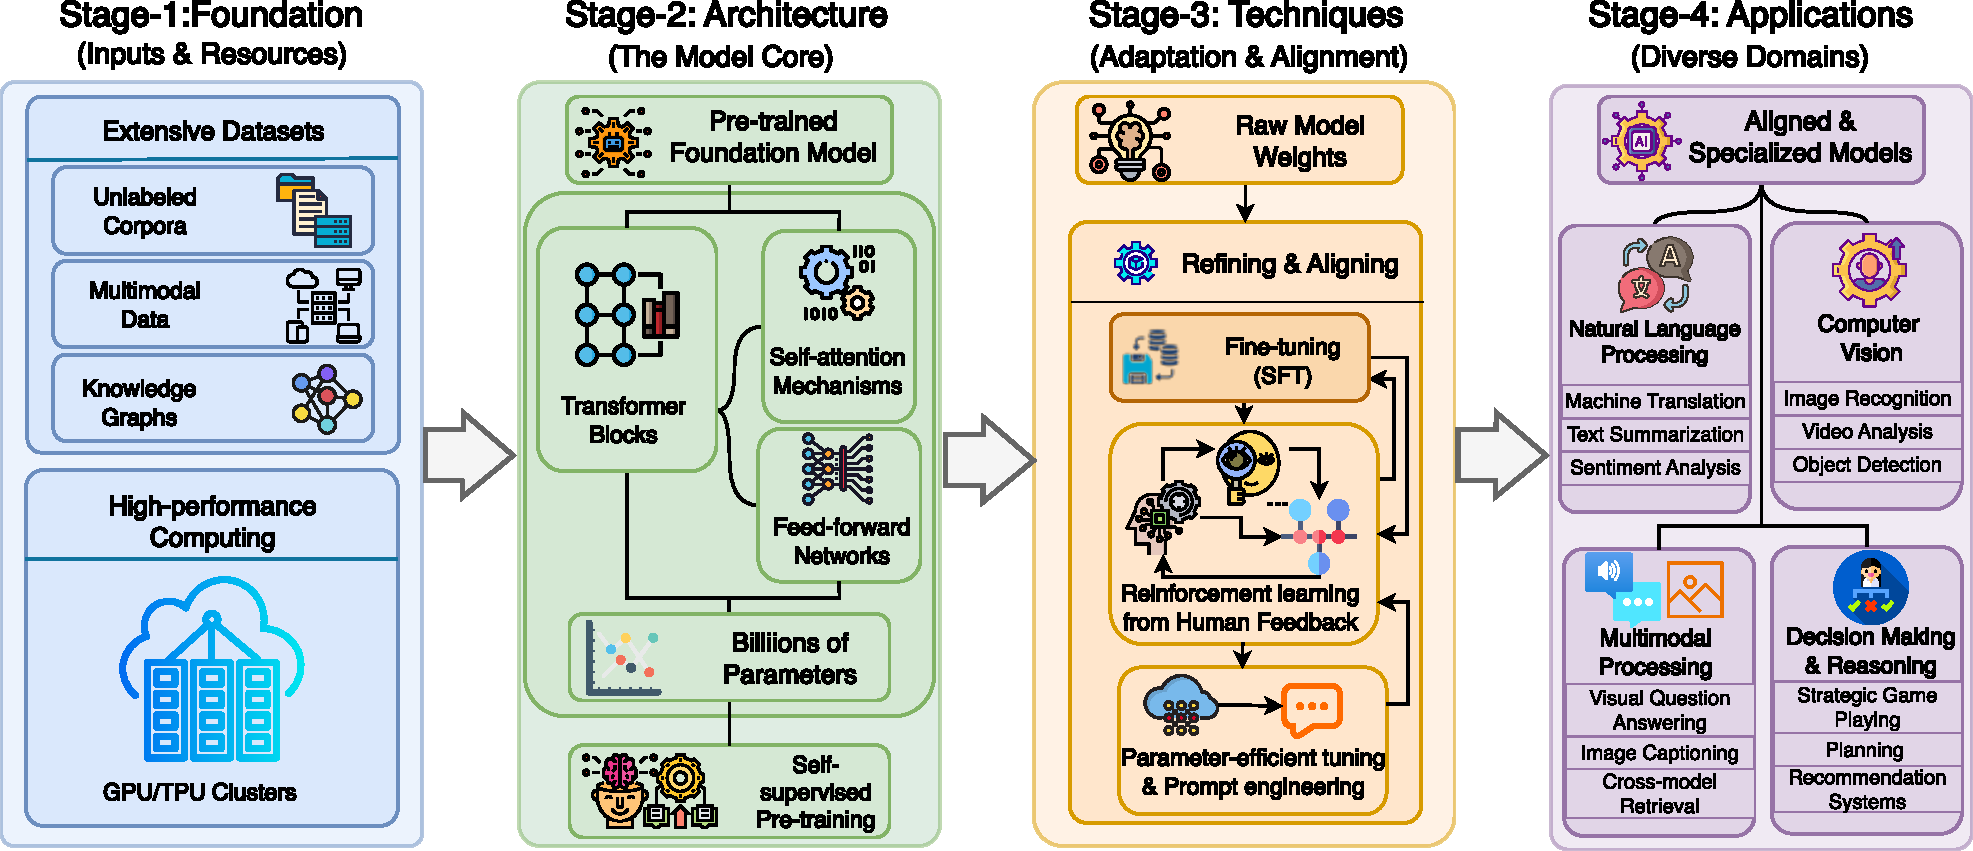
\includegraphics[width=0.80\linewidth]{large-model-v2.pdf}
\caption{An integrated framework of large models.}
\label{fig:large_model_arch}
\end{figure*}

One of the standout features of large models is their ability to perform well with minimal data input for specific tasks~\cite{yuan2022roadmap}. This capability is often referred to as few-shot or zero-shot learning. It mirrors human intelligence, where individuals generalize from limited examples to understand new concepts. After pre-training on comprehensive datasets, these models exhibit remarkable adaptability to novel tasks. They often require minimal labeled data for fine-tuning, with some instances achieving success solely through the provision of a concise prompt. This characteristic makes them particularly advantageous in fields where labeled data is scarce or difficult to obtain. To better understand and leverage the capabilities of these models, we classify large models into LLMs and LMMs. The feature comparison of these two models is shown in Table~\ref{tab:llm-lmm}. 


\textbf{Large Language Models:}
Large Language Models (LLMs) are advanced AI models designed to understand, generate, and manipulate human language~\cite{zhao2023survey,yang2024harnessinga,chang2024survey,han2024llm}. They have revolutionized NLP by leveraging vast datasets and complex architectures to perform a wide range of language tasks with high proficiency. Examples of widely known LLMs include GPT-3~\cite{brown2020language}, GPT-4~\cite{openai2024gpt4}, BERT~\cite{devlin2018bert}, and LLaMA~\cite{touvron2023llama}. These models are built on the Transformer architecture~\cite{vaswani2017attention}, which uses self-attention mechanisms to process sequential data efficiently and capture long-range dependencies in text. LLMs have significantly advanced NLP to enable improvements in diverse AI tasks such as language generation, translation, and question answering~\cite{chowdhary2020natural}.

One of the vital aspects of LLMs is \textquote{in-context learning}~\cite{brown2020language}, where the model generates text based on the context or prompt provided. This ability allows LLMs to produce coherent and contextually appropriate responses, making them ideal for applications involving interaction and conversation. Besides, the in-context learning leverages the model's capability to interpret and use the given context to predict subsequent text, which results in a seamless and relevant content generation. This feature is beneficial in applications such as chatbots (e.g., ChatGPT, Gemini), virtual assistants (e.g., Be My Eyes\footnote{\url{https://www.bemyeyes.com/}}), and automated content creation (e.g., Copy.ai\footnote{\url{https://www.copy.ai/}}), where maintaining the flow and relevance of the conversation is crucial. By continuously learning from the provided context, LLMs adapt to various styles and tones, which enhances their performance in generating text that closely mimics human language. Another essential aspect of LLMs is Reinforcement Learning from Human Feedback (RLHF)~\cite{christiano2017deep,ziegler2019fine}. This technique involves refining the model's performance by using human-generated responses as a form of reward. Through RLHF, the model learns from its mistakes and gradually improves its output quality. This approach is vital for developing models that provide more accurate and reliable responses over time. RLHF is particularly useful in scenarios that require high levels of accuracy and nuance, such as customer service interactions, content moderation, and personalized recommendations.


\textbf{Large Multimodal Models:}
Large Multimodal Models (LMMs) are designed to emulate the human brain's ability to process and integrate information from multiple sensory modalities, such as language, images, video, and audio~\cite{huang2024large}. These models aim to learn the correlations and complementarity between different types of data, a challenging task due to the inherent heterogeneity of multimodal data. The primary goal of LMMs is to align and integrate data from various modalities to enable the transfer of learned knowledge to a wide range of downstream tasks. LMMs employ diverse strategies to encode multimodal information. Image processing typically leverages pixel-level, patch-based, or vector-quantized modeling, whereas video analysis incorporates motion-based features and spatio-temporal modeling to capture dynamic content. Textual data is transformed via tokenization, sentence-level embeddings, or BERT-based encoding. These heterogeneous features are then integrated into LMM architectures, which are broadly classified into fusion or dual-encoder paradigms. 

Recent advances in computer vision have contributed significantly to the development of LMMs. For example, Vision Transformers (ViTs)~\cite{khan2022transformers} have emerged as a powerful tool for visual data representation. Likewise, Swin Transformer~\cite{liu2021swin} has shown state-of-the-art performance in handling complex visual information. These techniques are being integrated into LMMs to enhance their capability to process visual data alongside other modalities, enabling LMMs to understand and interpret visual information in combination with textual, auditory, and other forms of data. This integration allows LMMs to excel in applications such as image captioning, video analysis, and interactive AI systems where multimodal understanding is crucial. 

\begin{figure*}[ht!]
\centering
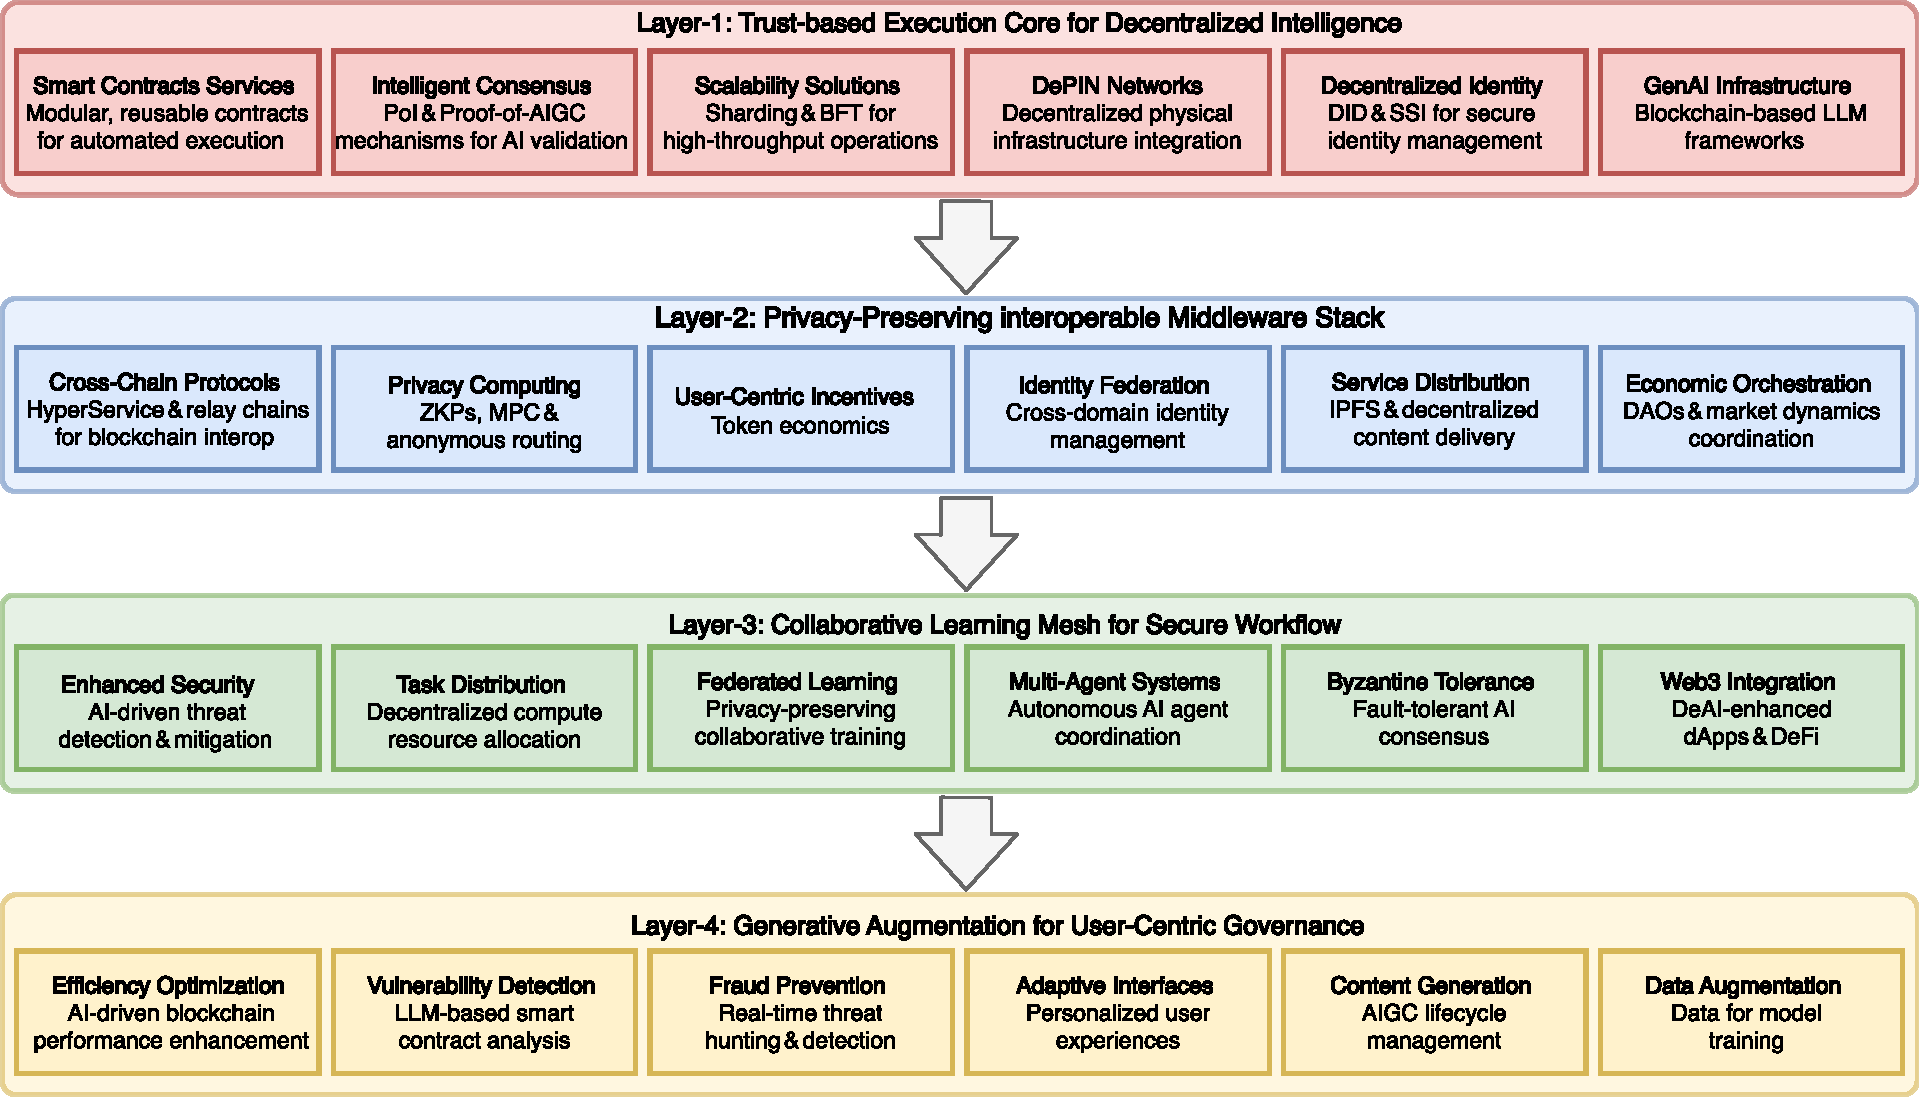
\includegraphics[width=0.90\linewidth]{interaction.pdf}
\caption{An overview of trust-to-augmentation framework.}
\label{fig:convergence}
\end{figure*}


	
\section{Trust-to-Augmentation: A Unified Framework for Decentralized Intelligence}
\label{sec:framework}
The convergence of decentralized and generative intelligence creates a natural layered architecture for decentralized intelligence systems. This section presents a unified trust-to-augmentation framework (as shown in Fig.~\ref{fig:convergence}) that organizes these technologies into four interconnected layers, providing a conceptual foundation for analyzing their integration and synergistic potential. Rather than viewing these technologies as isolated domains, the framework illustrates how they form a coherent stack in which each layer builds upon and enhances the capabilities of the layers beneath it.

To guide the reader, this section is organized as follows. First, we present the architectural principles and design rationale that motivate the layered structure. Second, we describe the interdependencies and data flows that connect the four layers. Third, we discuss instantiation patterns that map the framework to real-world systems. Fourth, we identify integration challenges and corresponding solutions. Finally, we consolidate these discussions in an insights subsection and provide a mapping table that explicitly links each framework layer to the detailed treatment in Section~\ref{sec:blockchain} through Section~\ref{sec:genai}.

\subsection{Architectural Principles and Design Rationale}
Building decentralized intelligence system requires addressing fundamental tensions between transparency and privacy, autonomy and coordination, and performance and security~\cite{cao2022decentralized}. Traditional approaches often sacrifice one property to achieve another. As a result, systems frequently excel in specific areas but remain vulnerable in others. Our framework emerged from analyzing these trade-offs across existing implementations and identifying how different technologies complement each other to resolve these tensions~\cite{yu2024toward,zeydan2025decentralizing}. Three core challenges drive the layered design:
\begin{itemize}
    \item \textbf{Verifiable Execution:} Requires execution where computations are independently verified without centralized trust;
    \item \textbf{Privacy under Transparency:} Preserves data privacy for AI operations and reconciles openness with confidentiality;
    \item \textbf{Coordinated Autonomy:} Autonomous agents maintain individual sovereignty while enabling collective intelligence.
\end{itemize}

Each layer of the framework addresses specific aspects of these challenges and incrementally builds upon the capabilities of the underlying tiers:
\begin{enumerate}
    \item \textbf{Layer 1 (Trust-based Execution):} Establishes a foundational trust infrastructure via immutable and verifiable computation, as discussed in Section~\ref{sec:blockchain};
    \item \textbf{Layer 2 (Privacy-Preserving Middleware):} Enables confidential computation and cross-chain interoperability as detailed in Section~\ref{sec:web3};
    \item \textbf{Layer 3 (Collaborative Learning Mesh):} Leverages trust and privacy primitives to facilitate distributed intelligence across organizational boundaries with a full discussion in Section~\ref{sec:deai};
    \item \textbf{Layer 4 (Generative Augmentation):} Introduces adaptive responses and user-centric interfaces to optimize the performance of the underlying layers with an in-depth analysis in Section~\ref{sec:genai}.
\end{enumerate}
This progression reflects computational requirements in distributed systems, where basic operations must be secured before complex behaviors can emerge. It also ensures that advanced GenAI functionality preserves the security and decentralization properties essential for trustless environments~\cite{luo2024survey,javadpour2024decentralized}.

\subsection{Layer Interdependencies and Data Flows}
Complex interdependencies between framework layers create emergent properties that exceed individual component capabilities. We describe these interdependencies in terms of upward dependencies, where higher layers rely on lower layers, and downward feedback, where advanced capabilities inform lower-level improvements.

\textbf{Upward Dependencies:} Smart contracts establish programmable trust that extends beyond transaction execution to validate AI model updates and regulate resource allocation~\cite{swain2025smart}. Intelligent consensus mechanisms further reinforce this trust by integrating proof-of-intelligence verification into the validation process~\cite{liu2024blockchainempowered}. Building on this foundation, privacy-preserving middleware employs cross-chain protocols and ZKPs to protect data integrity and confidentiality~\cite{qin2023web3based,kim2023moving}. These mechanisms enable secure communication channels for federated learning across organizational boundaries~\cite{shadmy2024reimagining}. Collaborative learning protocols rely on these channels to exchange and aggregate validated models, which are subsequently submitted for consensus verification. Byzantine fault-tolerant (BFT) mechanisms ensure robustness by preventing malicious interference during the model update process~\cite{shao2023decentralized,zheng2024decentralized}.

\textbf{Downward Feedback:} Generative augmentation forms dynamic feedback loops that continuously improve system capabilities. Large models analyze blockchain data, suggest adjustments to consensus parameters, and generate synthetic datasets for privacy-preserving training~\cite{brown2020language,zhao2023survey,bengesi2024advancements}. Bidirectional data flows enable continuous optimization across layer boundaries. For example, generative models identify consensus timing patterns that motivate parameter adjustments, and FL exposes privacy protocol inefficiencies that motivate middleware refinements~\cite{yuan2022roadmap}. In this way, intelligence enhancements propagate throughout all architectural layers.

These upward and downward relations provide the conceptual backbone for the layer-specific analysis in Sections~\ref{sec:blockchain} through~\ref{sec:genai}, where each layer is examined with respect to both its internal mechanisms and its cross-layer interactions.

\subsection{Framework Instantiation Patterns}
Different application requirements necessitate flexible instantiation approaches that range from complete implementations using all four layers to selective combinations tailored to specific needs~\cite{liu2023web3}. We categorize these patterns into three types: comprehensive, selective, and domain-specific instantiations.


\begin{itemize}

\item \textbf{Comprehensive Instantiation:} Comprehensive systems such as decentralized autonomous organizations integrate smart contract governance, cross-chain asset management, FL for decision-making, and generative AI for adaptive interfaces~\cite{li2024blockchain,shen2024artificial}. These implementations leverage all four layers and suit complex ecosystems that require full-stack decentralized intelligence.

\item \textbf{Selective Instantiation:} Selective implementations focus on a subset of layers when use cases or deployment constraints warrant a narrower scope. For example, financial applications can emphasize trust execution and privacy middleware, while content platforms can emphasize middleware and generative layers~\cite{duan2023metacube}. Hybrid approaches combine decentralized components with centralized resources in transitional deployments~\cite{tariq2025blockchain}.

\item \textbf{Domain-Specific Adaptation:} Domain-specific adaptations tailor the framework emphasis to particular requirements. Healthcare deployments prioritize privacy-preserving protocols and FL for sensitive medical data~\cite{thirunavukarasu2023large}, whereas supply chain applications emphasize trust execution and cross-chain interoperability to track goods across organizational boundaries~\cite{fasano2025exploring}. 

\end{itemize}

These instantiation patterns demonstrate framework flexibility in addressing diverse deployment constraints and application requirements while maintaining core architectural principles and appropriate security, privacy, and functionality trade-offs~\cite{huang2024large,khan2022transformers,vaswani2017attention}.

\textbf{Mapping to Surveyed Systems:} Several recent systems surveyed in later sections provide concrete instantiations that align closely with the four-layer design. For example, HyperService~\cite{liu2019hyperservice} enables cross-chain interoperability with verifiable execution for heterogeneous blockchains and services, which matches the privacy-preserving interoperable middleware layer. At the interface between trust execution and middleware, ZK-LLM~\cite{sun2024zkllm} offers zero-knowledge verifiability for LLM inference through dedicated proof protocols, and demonstrates that large models can be audited without exposing sensitive data. BasedAI~\cite{wellington2024basedai} illustrates an end-to-end realization that combines encrypted LLM computation, incentive-driven participation, and decentralized service delivery, and confirms that privacy preservation, collaborative learning, and generative augmentation can operate together in practice. Trust-free inference platforms such as SAKSHI~\cite{bhat2023sakshi} highlight the role of verifier-style agents and proof-of-inference mechanisms within collaborative learning meshes, and reinforce the need for explicit verification loops in decentralized intelligence architectures. More recently, VeriLLM~\cite{wang2025verillm} proposes a lightweight framework for publicly verifiable decentralized LLM inference that complements ZK-LLM and shows that proof systems can scale to realistic model deployments. These systems support the generality of the trust-to-augmentation framework and indicate that existing deployments map naturally onto its layers.

\subsection{Integration Challenges and Solutions}
Implementing comprehensive decentralized intelligence systems introduces architectural complexities that require careful balance between competing requirements~\cite{hassan2025enabling}. We organize these challenges into four categories: scalability, semantic consistency, economic alignment, and governance coordination.

\begin{itemize}

\item \textbf{Scalability:} Scalability challenges arise when consensus mechanisms must validate both traditional transactions and computationally intensive AI operations~\cite{thong2025know,feng2025efficient}. Hierarchical consensus and similar mechanisms address this issue by reserving global verification for critical trust operations and relying on local validation for routine AI computations.

\item \textbf{Semantic Consistency:} To maintain semantic consistency across diverse data representations, systems require standardized interface protocols and canonical formats~\cite{far2024third}. Cross-layer optimization must ensure that performance improvements in one component do not degrade dependent system functionality~\cite{wan2024web3}.

\item \textbf{Economic Alignment:} Economic incentive alignment becomes complex when participants operate across multiple layers with potentially competing interests~\cite{qian2024alibaba}. Multi-layer tokenomics that reward ecosystem-wide contributions and reputation mechanisms that track behavior across framework components provide partial mitigation.

\item \textbf{Governance Coordination:} Governance coordination involves managing protocol upgrades across interconnected systems through mechanisms that enable routine decisions within individual layers while requiring cross-layer consensus for structural changes~\cite{christiano2017deep,ziegler2019fine}. Successfully addressing these integration challenges demonstrates how structured architectural frameworks provide robust foundations for scalable decentralized intelligence systems that preserve security, privacy, and autonomy properties essential for trustless environments~\cite{dorri2018multi}.

\end{itemize}

These four challenge classes recur as cross-cutting concerns throughout Sections~\ref{sec:blockchain} through~\ref{sec:genai}, and they motivate several of the open research directions discussed in Section~\ref{sec:future}.


\subsection{Insights}
The trust-to-augmentation framework provides a structured lens for analyzing the convergence of decentralized and generative intelligence. By organizing the technological landscape into four interdependent layers, the framework clarifies how foundational trust mechanisms enable progressively more sophisticated capabilities, from privacy-preserving computation to collaborative learning and generative augmentation. The key insight is that these layers do not operate as independent silos but form a mutually reinforcing stack: trust-based execution provides the verifiable substrate for privacy middleware; privacy guarantees enable secure collaborative learning; and collaborative intelligence supplies signals that generative systems use to propose improvements, which then propagate back to the lower layers through feedback loops.



\section{Trust-based Execution for Decentralized Intelligence} \label{sec:blockchain}
While blockchain provides an immutable root-of-trust for data storage, decentralized intelligence demands a more comprehensive trust model that includes the execution of AI-driven logic. This section discusses how smart-contract services and intelligent consensus mechanisms such as Proof-of-Intelligence (PoI) turn the ledger into a verifiable compute substrate. We also examine scalability, decentralized identity, and DePIN-based hardware networks that supply off-chain resources while inheriting on-chain guarantees. Finally, we discuss infrastructure patterns that allow GenAI and Web3 applications to plug into this trust-based execution layer without sacrificing performance or privacy. A comparative analysis of relevant literature is provided in Table~\ref{tab:block} with a focus on various frameworks, solutions, privacy measures, interoperability, and evaluation metrics.

\begin{table*}[ht!]
\centering
\caption{Comparison of literature focused on trust-based execution for decentralized intelligence.}
\label{tab:block}
\footnotesize
\selectfont
\setlength\tabcolsep{0.6pt}
\begin{tabularx}{\linewidth}{
>{\hsize=0.05\hsize}Z
>{\hsize=0.10\hsize}Z
>{\hsize=0.12\hsize}Z
>{\hsize=0.10\hsize}Z
>{\hsize=0.10\hsize}Z
>{\hsize=0.11\hsize}Z
>{\hsize=0.11\hsize}Z
>{\hsize=0.14\hsize}Z
>{\hsize=0.21\hsize}Y}
\toprule 
\textbf{Ref.} & \textbf{Arch.} & \textbf{Solution} & \textbf{Privacy} & \textbf{Int.} & \textbf{Inter.} & \textbf{Gov.} & \textbf{Evaluation} & \multicolumn{1}{c}{\textbf{Remarks}} \\\midrule

~\cite{liu2024blockchainempowered} & Blockchain & Lifecycle management & Proof-of-AIGC & Edge computing & Edge devices & User-driven control & Reputation value, task ratio & \makecell[l]{i) Protect AIGC copyright \\ii) Incentivize AIGC} \\\hline 

~\cite{butincu2024design} & Blockchain, Web3 & SSI-based storage & \makecell[c]{Distributed \\ledger} & Cloud mapping & Cross-platform & User-driven control & Trust, privacy, scalability & \makecell[l]{i) Emphasize user privacy \\ii) Eliminate failure points} \\\hline 

~\cite{fan2023towards} & DePIN & Storage, computation & \makecell[c]{zk-Rollup, \\TEE} & Sequencer & Cross-chain & On-chain, off-chain & Scalability, Data availability & \makecell[l]{i) Rollup-based scalability \\ii) Data integrity via ZKP} \\\hline 

~\cite{heiss2024towards} & DePIN & CDR & ZKP & dApps & SSI systems & dApp Initiator &  Range, membership, equality & \makecell[l]{i) Data confidentiality \\ii) Device verification} \\\hline 

~\cite{liu2024decentralised} & Blockchain & Accountability & Permissioned blockchain & LLM & Identity registry and recording integration & Decision-making & Response validation, incentive distribution & \makecell[l]{i) Enhanced accountability \\ii) RAI for governance} \\\hline 
 
~\cite{liu2024ssdid} & Blockchain, Web3 & Identity verification & BFT & Sharding & Cross-chain & User-managed identity control & Verification accuracy, privacy protection & \makecell[l]{i) Strengthen privacy\\ii) Support cross-platform\\ identity} \\\hline 

~\cite{sun2024smart} & Blockchain, Web3 & SCaaS & Smart contract & EVM & Cross-platform & Community-driven & Storage reduction, Cost efficiency & \makecell[l]{i) Reuse smart contract \\ii) Web3 development} \\\bottomrule
\end{tabularx}
\begin{tablenotes}
\item \textbf{Arch.}=Architecture; \textbf{Int.}=Integration; \textbf{Inter.}=Interoperability; \textbf{Gov.}=Governance; \textbf{SSI}=Self-Sovereign Identity; \textbf{TEE}=Trusted Execution Environment; \textbf{CDR}: Credential-based device registration; \textbf{AIGC}=Artificial Intelligence-Generated Content; \textbf{RAI}=Responsible AI; BFT=Byzantine fault tolerance; \textbf{SCaaS}=Smart Contracts as a Service; \textbf{EVM}=Ethereum Virtual Machine.  
\end{tablenotes}
\end{table*}

\subsection{Smart Contracts as a Service}
Smart contracts provide automated and trustless agreements that execute predefined actions when specified conditions are met. They facilitate secure and transparent interactions between decentralized applications by enabling the execution of intelligent algorithms, management of data exchanges, and distribution of computational resources without the need for intermediaries. This approach ensures increased efficiency and reduced operational costs. For example, Sun et al.~\cite{sun2024smart} introduce the Smart Contract as a Service (SCaaS) paradigm to address critical challenges within the Web3 ecosystem, such as redundant smart contract development, storage limitations, and increased development costs. By leveraging the reusability and composability of smart contracts, SCaaS promotes a modular approach, treating contracts as building blocks (similar to LEGO bricks) that can be combined to create more complex and interoperable applications. This paradigm significantly reduces development overhead and alleviates on-chain storage demands.

On the other hand, Liu et al.~\cite{liu2024decentralised} propose an AI-enabled decentralized governance system through the lens of SCaaS. Smart contracts are leveraged to automate and manage critical governance tasks, including identity management, data integrity verification, incentive distribution, and response validation. The SCaaS-based framework facilitates accountability and proper management of decision rights across diverse stakeholders. It also highlights the potential of blockchain to provide a robust and programmable infrastructure for the governance of responsible AI (RAI)~\cite{lu2024responsible,berman2024scoping}. However, the work is primarily conceptual and lacks empirical validation, which raises concerns about practical implementation, trust, and transparency among stakeholders. 
%
Furthermore, Huang et al.~\cite{huang2024advancing} propose a decentralized framework titled SMART to enhance smart contracts with AI capabilities. The SMART framework leverages a joint on-chain and off-chain execution model, utilizing Trusted Execution Environments (TEEs)~\cite{sabt2015trusted}. By decentralizing AI capabilities, SMART facilitates the development of sophisticated Web3 applications, such as AI-driven content moderation in social media, dynamic non-playable characters in gaming, and enhanced risk assessment in DeFi~\cite{tanaka2024taxonomy} It also employs distributed attestation services and secret key provisioning to guarantee the integrity and confidentiality of AI models during execution.


\subsection{Intelligent Consensus Mechanisms}
Blockchain-based intelligent consensus mechanisms enhance decision-making and value creation in decentralized systems. Unlike traditional approaches (e.g., PoW, PoS), these mechanisms leverage advanced computational techniques to evaluate network efficiency and integrity and to align incentives accordingly. By incorporating DeAI and GenAI, these protocols redefine node participation and contribution in blockchain networks. For example, Proof-of-AIGC~\cite{liu2024blockchainempowered} protects the ownership and copyright of AI-generated content by registering it on the blockchain and enabling verification as an original work, which reduces tampering and plagiarization. This protection is important because AI-generated content, treated as non-fungible digital property, remains highly susceptible to these attacks.

Proof of Intelligence (PoI) is another unique consensus mechanism that leverages the Bittensor network\footnote{\url{https://bittensor.org/}} to incentivize valuable contributions in the form of ML models~\cite{rao2020bittensor}. The Bittensor network is a decentralized platform designed to create, share, and monetize ML models collaboratively. It functions by utilizing its native blockchain to establish a community-driven environment, where participants contribute to training models while being rewarded for their work. This ecosystem not only fosters the exchange of AI expertise but also ensures that valuable contributions are recognized and rewarded fairly, leading to more sophisticated models and improved overall network intelligence. Unlike traditional PoW or PoS mechanisms that rely on computational power or coin ownership, PoI rewards nodes based on the intellectual merit of their contributions. Nodes compete by deploying ML models, and the accuracy and value of their outputs determine their eligibility to add new blocks to the blockchain and earn rewards in TAO tokens. In an integrated scenario, Proof-of-AIGC and PoI can work together to ensure both the quality and originality of digital products while incentivizing innovative contributions. These intelligent consensus mechanisms promote an environment where contributions are verified for their authenticity and intellectual value while being rewarded accordingly. Such integration is crucial in creating a self-sustaining system where high-quality digital assets are developed, protected, and utilized effectively.


\subsection{Scalability and Decentralized Identity}
Scalability and decentralized identity (DID) are essential for enabling secure and efficient identity management in decentralized systems. Blockchain addresses the scalability and interoperability challenges in DID systems by providing a tamper-proof distributed ledger to facilitate trust across domains. For instance, Liu et al.~\cite{liu2024ssdid} propose a multilayer architecture to address the scalability, security, and compatibility challenges associated with existing Web3-based DID systems. Their architecture leverages sharding~\cite{thong2025know} and Byzantine Fault Tolerance (BFT) consensus mechanism to partition identity management nodes into distinct shards. This partitioning significantly enhances both scalability and system performance by organizing identity management nodes efficiently. Leader shards and a main chain work in coordination to establish trust and streamline coordination across different domains. Additionally, the use of Merkle trees allows for seamless cross-domain credential verification, ensuring security and traceability. As a result, this architecture achieves high throughput and low latency, dramatically improving the ability of DID systems to manage large-scale transactions without dependence on a central authority.

Another approach to overcoming the limitations of centralized identity systems has been proposed by Butincu et al.~\cite{butincu2024design}, who introduce a multi-layered architecture leveraging DIDs and Self-Sovereign Identities (SSIs). Their design emphasizes scalability through a decentralized structure, which consists of entry, core, and storage layers. This allows the system to maintain resilience, flexibility, and user control across a wide range of applications. The proposed front-end and back-end blockchain configurations ensure that identity verification processes are secure and scalable without relying on single points of failure. This enhances system robustness, improves data privacy, and offers the potential for broad cloud integration, all critical for supporting large-scale identity systems in diverse environments.

\subsection{Decentralized Physical Infrastructure Network}
The Decentralized Physical Infrastructure Network (DePIN) is an innovative network architecture developed to overcome the shortcomings of traditional centralized infrastructure systems, such as data privacy vulnerabilities, service interruptions, and high expansion costs. As shown in Fig.~\ref{fig:depin_arch}, DePIN decentralizes the control and management of physical devices by leveraging blockchain~\cite{ballandies2023taxonomy,lin2024decentralized}. Here, blockchain acts as the core infrastructure supporting decentralized control, governance, and data management across the network. This integration ensures tamper-proof and transparent data records to enhance security and trustworthiness~\cite{ballandies2023taxonomy}. By employing Web3 governance mechanisms such as DAOs, DePIN ensures transparent and democratic decision-making processes to enhance trust and security within the blockchain network~\cite{fan2023towards}. 

\begin{figure*}[!t]
\centering
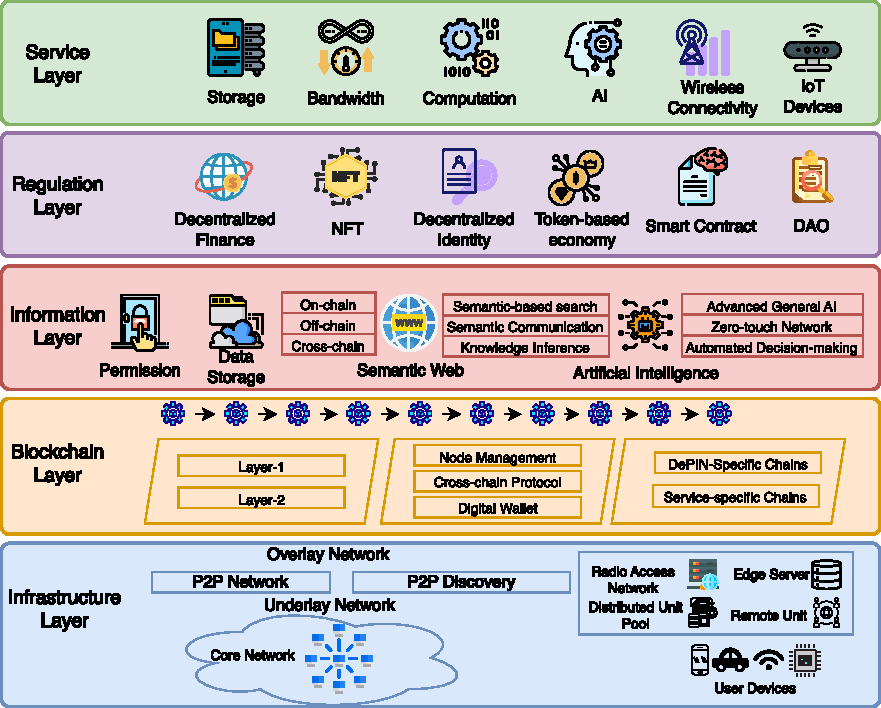
\includegraphics[width=0.70\linewidth]{depin_arch.pdf}
\caption{Layered architecture of DePIN framework.}
\label{fig:depin_arch}
\end{figure*}

DePIN incentivizes participants through token mechanisms to encourage active involvement and resource sharing~\cite{chiu2024depin}. For example, Fan and Xu~\cite{fan2023towards} introduce a rollup-oriented scalable architecture for DePINs by leveraging blockchain, IoT, and tokenomics to innovate Web3-based IoT business models. The authors uniquely integrate zk-Rollups and TEEs to augment both scalability and security in order to facilitate resource sharing among large-scale DePIN applications. They propose a novel architecture that tackles scalability issues through off-chain computations and ZKPs. The architecture includes Sovereign Smart Devices (SSDs) for data collection, a data availability layer for short-term data storage, a Decentralized Sequencer Network (DSN) for consensus and data storage, a decentralized aggregator network for generating aggregated ZKPs, and a layer-1 blockchain for verification and settlement. 

On the other hand, Heiss et al.~\cite{heiss2024towards} address the challenge of establishing trust in DePINs within the Web3 ecosystem. The authors introduce a credential-based device registration mechanism that uses ZKPs to protect confidential device attributes while ensuring on-chain verifiability. They also propose a system that integrates W3C-based verifiable credential model with zkSNARKs~\cite{nitulescu2020zk} to verify device credentials without disclosing sensitive information. The system model features device attribution, registration conditions, and credential issuers, and includes a three-phase methodology of attestation, setup, and registration. The authors also provide a prototypical implementation of the proposed mechanism using ZoKrates~\cite{eberhardt2018zokrates} and conduct experiments to evaluate the performance of zkSNARKs with different proof systems such as Groth16~\cite{groth2016size} and Marlin~\cite{chiesa2020marlin}.

In terms of functionality and operation management, Lin et al.~\cite{lin2024decentralized} propose a hierarchical DePIN architecture composed of several layers: application, governance, data, blockchain, and infrastructure layers. Each of these layers is designed to ensure the network's efficiency, security, and scalability. The application layer offers diverse, long-lived services, while the governance layer utilizes decentralized decision-making mechanisms, such as DAOs and smart contracts, to maintain transparency and democratic control. Consequently, the data layer is focused on secure, intelligent data management through advanced encryption and semantic technologies. Furthermore, the blockchain layer integrates general-purpose and specific blockchain solutions, which form the backbone of decentralized economics and governance. Finally, the infrastructure layer provides essential communication, computing, and storage resources through a scalable overlay and underlay network structure.


\subsection{Infrastructure for GenAI and Web3}
Blockchain technology is emerging as a key platform for fostering the development of collaborative AI models and creating a decentralized marketplace for GenAI and Web3. This is enabled by blockchain's decentralized infrastructure that supports secure data sharing and collaborative intelligence across distributed systems. For instance, Gong~\cite{gong2023dynamic} proposes a novel decentralized LLM framework that leverages blockchain to empower LLMs with dynamic capabilities. The proposed framework facilitates the transition from centralized to decentralized LLM architectures to support continuous and real-time training. The author further investigates how blockchain underpins decentralized datasets and economic incentives to foster an open and collaborative platform for LLM model contributors and validators. Likewise, Wen et al.~\cite{wen2024generative} propose an incentive mechanism that utilizes blockchain to perform data synthesis, data augmentation, and anomaly detection in a generative IoT (GIoT) environment. The proposed blockchain layer securely manages the GIoT networks to ensure transparency in resource trading and reputation management, which discourages malicious behavior and maintains data integrity. In addition, this layer works in conjunction with GDMs to ensure that the optimal incentive mechanisms derived through GDMs are securely implemented and that the implementation remains transparent and immutable. Overall, the study suggests an integrated framework but does not detail how to ensure interoperability across various platforms and devices within the GIoT ecosystem.

As for Web3 infrastructure, Liao et al.~\cite{liao2024graph} propose a graph-based attention network (GAT) to optimize block propagation. The authors introduce the Age of Block (AoB) as a novel metric for assessing block propagation efficiency and employ a reputation mechanism based on subjective logic models to enhance miner reliability. By integrating GAT with reinforcement learning (RL), the framework captures complex relationships within the miner network and optimizes the block propagation trajectory. Additionally, the use of multi-head attention within the GAT architecture allows for a nuanced exploration of miner interactions, leading to a reduction in block propagation time and an increase in miner reputation scores.

\subsection{Insights}
The convergence of smart contracts as a service, intelligent consensus mechanisms, scalability solutions, DePIN architectures, and GenAI infrastructure establishes blockchain as a comprehensive trust-based execution platform for decentralized intelligence. This integration creates an adaptive ecosystem where blockchain transcends traditional ledger functionality to become a programmable trust infrastructure that autonomously validates AI contributions, manages computational resources, and orchestrates intelligent services across distributed networks. The synthesis of AI-driven consensus protocols (e.g., PoI and PoAIGC) with modular smart contract architectures and scalable identity management systems demonstrates how blockchain can provide cryptographic guarantees for AI system integrity while enabling seamless service composition and resource allocation in decentralized environments.

\begin{table*}[!t]
\centering
\caption{Comparison of studies on privacy-preserving interoperable middleware stack.}
\label{tab:web3}
\footnotesize
\selectfont
\setlength\tabcolsep{0.6pt}
\begin{tabularx}{\linewidth}{
>{\hsize=0.05\hsize}X
>{\hsize=0.10\hsize}Z
>{\hsize=0.10\hsize}Z
>{\hsize=0.09\hsize}Z
>{\hsize=0.11\hsize}Z
>{\hsize=0.10\hsize}Z
>{\hsize=0.11\hsize}Z
>{\hsize=0.11\hsize}Z
>{\hsize=0.06\hsize}Z
>{\hsize=0.20\hsize}Y}
\toprule 
\textbf{Ref.} & \textbf{Arch.} & \textbf{Solution} & \textbf{Apps} & \textbf{Tasks} & \textbf{Feature} & \textbf{Metrics} & \textbf{Source} & \textbf{SCA} & \multicolumn{1}{c}{\textbf{Remarks}} \\\toprule

~\cite{huang2024advancing} & TEE & Privacy protection & DAO, dApp & Content moderation & Transformer & Latency, scalability & \ding{53} & \ding{51} & \makecell[l]{i) Enhanced user privacy \\ii) dApp compatibility} \\\hline 
 
~\cite{liao2024graph} & Blockchain & Propagate blocks & dApps & dApps collaboration & RL, GAT & Reputation latency & \ding{53} & \ding{53} & \makecell[l]{i) Propagation reliability \\ii) Miner selection} \\\hline 
 
~\cite{gunathilaka2024defitrust} & Blockchain & Scam detection & DeFi, DAO & Token identification & BERT & PR, F1 & Ethereum logs & \ding{51} & \makecell[l]{i) Detection accuracy \\ii) Limited to token scams} \\\hline 

~\cite{si2024understanding} & User interaction & Risk assessment & User control & Risk management & \ding{53} & Feedback ratio & \ding{53} & \ding{53} & \makecell[l]{i) User-centric security \\ii) Lack technical depth} \\\hline 
 
~\cite{torres2023your} & DeFi & Privacy analysis & dApp, wallet & User tracking prevention & \ding{53} & Leaks ratio & dApps, wallets & \ding{51} & \makecell[l]{i) Wallet privacy risks \\ii) Focus third-party leaks} \\\hline 

~\cite{wu2023know} & Motif & Semantic extraction & DeFi, NFT & Transaction classification & \ding{53} & PR, RE, AC & Etherscan transactions & \ding{51} & \makecell[l]{i) Supports multi-tasking \\ii) Semantic complexity} \\\hline 
 
~\cite{zhou2024capsuleformer} & Capsule & Classify traffic & dApps & Encrypted traffic analysis & Transformer & AC, F1 & Ethereum \& BNB logs & \ding{51} & \makecell[l]{i) Classification accuracy \\ii) Encryption complexity} \\\hline 

~\cite{zhou2023harnessing} & Bitcoin & Social analysis & Social media & Content moderation & \ding{53} & Transaction time & Users, posts, actions & \ding{51} & \makecell[l]{i) Economic inequalities \\ii) Lack moderation}\\\bottomrule

\end{tabularx}
\begin{tablenotes}
\item \textbf{SCA}=Source Code Availability; \textbf{TEE}=Trusted Execution Environment; \textbf{GAT}=Graph Attention Network; \textbf{RL}: Reinforcement Learning; \textbf{AC}=Accuracy; \textbf{PR}=Precision; \textbf{RE}=Recall; \textbf{F1}=F1-Score; \textbf{BNB}=Binance.
\end{tablenotes}
\end{table*}


\section{Privacy-Preserving Interoperable Middleware Stack} \label{sec:web3}
With a trusted execution core in place, decentralized systems next require a fabric that can route value, data, and identity across heterogeneous chains and off-chain services without exposing sensitive information. This section surveys interoperability protocols, privacy-preserving compute techniques, and incentive mechanisms that align users and validators. We discuss the cross-domain identity management and token-driven market dynamics that together form a middleware stack linking isolated networks into a cohesive and privacy-aware ecosystem. A comparative analysis is presented in Table~\ref{tab:web3} with a focus on architecture, solutions, applications, tasks, features, evaluation metrics, data sources, source code availability, and key remarks.

\subsection{Interoperability with Blockchain}
Web3 plays a crucial role in promoting interoperability between blockchain networks, allowing different systems to communicate and transact seamlessly (as shown in Fig.~\ref{fig:web3_layer}). This interoperability is further supported by layer-2 (L2) solutions (e.g., Arbitrum~\cite{kalodner2018arbitrum}, Optimism\footnote{\url{https://www.optimism.io/}}, Polygon~\cite{web-polygon}), which address the inherent scalability limitations of traditional blockchain. By enabling diverse blockchain systems to interoperate and scale, Web3 paves the way for broader adoption and the development of more complex applications~\cite{hassan2023enabling}.

\begin{figure}[ht!]
\centering
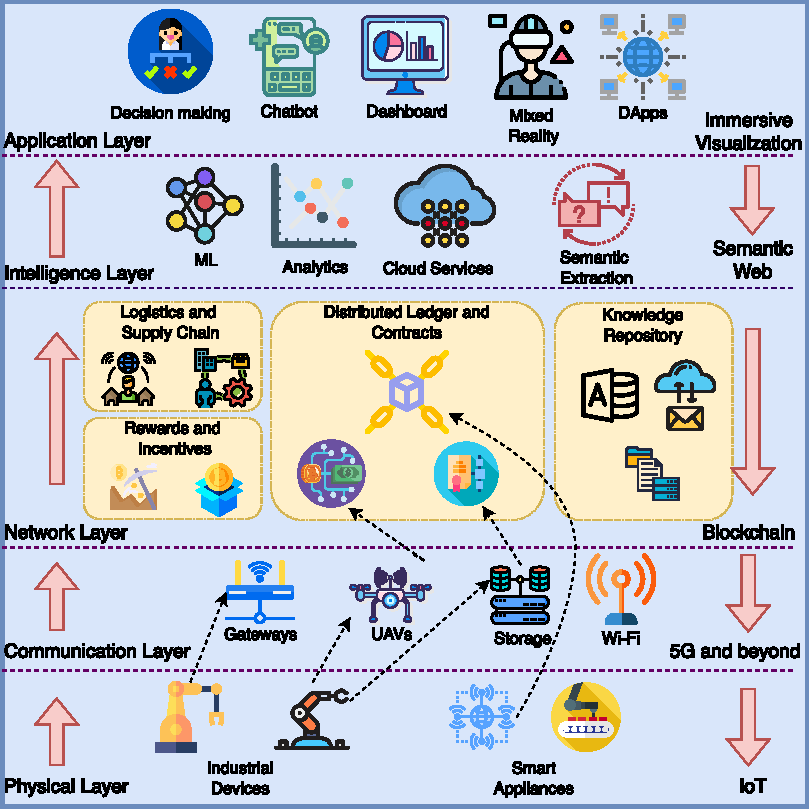
\includegraphics[width=\linewidth]{web3_layered.pdf}
\caption{Interoperability of Web3 components.}
\label{fig:web3_layer}
\end{figure}

In terms of interoperability and verifiability, Liu et al.~\cite{liu2021make} introduce an innovative interoperability platform named HyperService to connect heterogeneous blockchains and centralized state publishers into a unified computing framework. HyperService features a developer-facing programming framework that utilizes a unified state model and a high-level programming language to facilitate cross-chain dApp development. Additionally, it includes a blockchain-facing cryptography protocol to ensure the secure and verifiable execution of dApps across multiple blockchains. The prototype implementation of HyperService (approximately 62,000 lines of code) demonstrates its practicality and scalability through experiments with cross-chain dApps. Furthermore, Zhang et al.~\cite{zhang2022web} identify cross-chain interoperability as a critical challenge and propose a framework incorporating global user identities, verifiable state ledgers, and relay chains to facilitate the exchange of information and assets across diverse platforms. While acknowledging the potential of existing solutions such as hashed time-lock contracts (HTLC)~\cite{web-htlc}, the authors highlight the security and efficiency limitations of relay chains. To address these shortcomings, they advocate for alternative cross-chain protocols such as Cosmos~\cite{kwon2019cosmos} and Polkadot~\cite{wood2016polkadot} to bridge disparities in consensus mechanisms (e.g., PoW, PoS), smart contract languages, and access control policies.

Chi et al.~\cite{chi2023networking} address the critical challenge of interoperability among parallel Web3-based metaverses. The authors propose utilizing knowledge graphs and decentralized ML to facilitate data exchange in the metaverse while preserving data privacy. The study explores various scenarios, including multi-blockchain, single-blockchain, and intra-metaverse contexts, to highlight the importance of data integrity, scalability, and privacy-preserving knowledge sharing. However, the research is limited by the absence of standardized data formats and its reliance on centralized servers due to the high storage costs associated with blockchain and the complexities of decentralized knowledge inference without a centralized coordinator. On the other hand, Wu et al.~\cite{wu2023know} present a novel motif-based transaction semantics method to address the need for real-time and generic extraction of transaction semantics in the rapidly evolving Web3 ecosystem. The authors first develop a high-performance RPC-based extract, transform, load (ETL) tool to efficiently extract blockchain transaction data. They then use network motifs to represent these transactions as semantic vectors, enhancing classification and analysis tasks across different blockchain platforms. While the method is designed for account-based blockchains, scaling according to Web3's increased volume and diverse transactions presents challenges such as data consistency, computational efficiency, and semantic adaptability.

\subsection{Privacy-Preserving Decentralized Computing}
Privacy-preserving decentralized computing addresses the need for secure and confidential data processing in Web3 environments. Techniques such as asymmetric encryption~\cite{simmons1979symmetric}, secure multi-party computation~\cite{du2001secure}, and anonymous routing~\cite{shirazi2018survey} can be applied to achieve a balance between computational efficiency and robust privacy protection, enabling trustworthy operations across various applications. For example, Guo et al.~\cite{guo2023blockchain} introduce a blockchain-assisted privacy-preserving data computing architecture that combines state channels and onion routing. This solution aims to address the limitations of existing Web3 platforms by enhancing trust and privacy in distributed computing environments. The authors propose a secure computing sandbox where computations are executed collaboratively and off-chain to mitigate the computational overhead associated with consensus mechanisms. Experimental results demonstrate improved privacy protection with acceptable latency compared to traditional and other privacy-focused approaches. However, the research acknowledges limitations such as an additional communication overhead, resource constraints, and the complexity of integrating multiple technologies, which may hinder scalability and efficiency in large-scale Web3 applications.

In terms of resource allocation, Qiu et al.~\cite{qiu2023fog} introduce a novel fog-assisted, blockchain-based radio access network designed to leverage decentralized computing and enhance resource allocation efficiency for Web3 applications. By integrating fog computing, the authors enable distributed storage and processing at the network edge to reduce latency and improve real-time data handling. The architecture incorporates a matching game-based computing offloading strategy to optimize resource allocation between fog-assisted user equipment and access points. This strategy minimizes system costs by considering latency, energy consumption, and transaction expenses, thereby effectively managing computing resources for demanding Web3 services.

\subsection{User-centric Incentives and Interactions}
The shift toward decentralized systems emphasizes empowering users with greater control over their data, privacy, and digital interactions. In the Web3 ecosystem, user-centric incentives and adaptive interactions are designed to enhance engagement through personalized, secure, and efficient services. These frameworks often integrate AI to analyze user behavior and optimize services in real time. For instance, Zhang et al.~\cite{zhang2023ai} propose a decentralized AI-enabled user experience within a Web3-enabled metaverse framework. The authors aim to empower users by restoring control over their data and enhancing privacy through a blockchain-backed secure storage layer. This is complemented by an AI-driven smart decision layer that personalizes user interactions and improves service delivery through the analysis of user data and behavior. The integration of edge and cloud servers further enhances the framework to ensure low-latency and high-reliability decentralized experiences in a highly interactive, user-centered digital environment. Consequently, Liu et al.~\cite{liu2023web3} explore the integration of Artificial General Intelligence (AGI)~\cite{goertzel2014artificial} within the Web3 ecosystem to establish a digital environment that is adaptive, efficient, and centered around the user. The environment enables AGI to be delivered through an AI-as-a-Service (AIaaS) model. This model acts as a catalyst for zero-touch services that enhance data accessibility and user ownership. Furthermore, the AIaaS framework not only supports the development of AGI but also facilitates seamless and continuous service adaptation and optimization of the Web3 ecosystem. This approach enhances service delivery and management, making Web3 more responsive and tailored to individual user contexts.

DeScan~\cite{de2024descan} provides censorship-resistant indexing services to tackle centralization, transparency, and fairness issues. It converts Web3 transactions into triplets by utilizing a Skip Graph data structure~\cite{aspnes2007skip}. These triplets are then distributed across a peer-to-peer network to ensure efficient query processing and scalability. Performance evaluation shows that DeScan maintains its functionality with up to 25\% adversarial and 35\% unresponsive peers without significant performance loss. Regarding user behavior analysis and interactions in Web3, Si et al.~\cite{si2024understanding} propose a comprehensive user interaction framework encompassing blockchain, dApps, online communities, and off-chain cryptocurrency platforms. The authors explore four categories of user-adopted mitigation strategies: risk assessment, aversion to risk, diversification of investments, and acceptance of risk. Through observational research and semi-structured interviews, they analyze how users engage with these components and identify the security concerns (e.g., social engineering attacks) they face. The study explores user behavior regarding the challenges they encounter and the strategies they employ to navigate the complex security landscape of Web3.

In regard to handling sensitive user information, Torres et al.~\cite{torres2023your} present a comprehensive analysis of the privacy implications associated with dApps and wallet extensions. Their research findings indicate that 1,325 out of the top 100,000 websites and third-party scripts use wallet APIs to monitor user behavior. Additionally, the analysis reveals that a substantial proportion of 211 out of 616 dApps and 13 out of 100 wallet extensions leak user wallet addresses to third parties. The authors also propose countermeasures to enhance wallet privacy by implementing more robust permission systems, that require explicit user consent before sharing any wallet information with dApps or third parties.


\subsection{Identity Management and Service Distribution}
Web3 introduces decentralized identity management solutions that provide secure and verifiable digital identities for users. These solutions enhance privacy and security by allowing users to control their identity information and selectively share it with trusted parties.
%
For example, Xu et al.~\cite{xu2023decontroller} introduce a three-tier identity management framework, deController, to enhance privacy and security within the Web3 ecosystem. Built upon underlay and overlay networks, deController offers an identity management service. This includes real-world identities for users' confidential information, blockchain addresses for network operations, and application-specific identities for various Web3 services. The framework also employs ZKPs and verifiable random functions to facilitate secure interactions while preserving user anonymity and data integrity in order to address the critical challenges in decentralized identity management. 

In regard to decentralized service distribution, Costa et al.~\cite{costa2023studying} investigate the challenges and dynamics of identity management and data sharing within the Web3-based IPFS ecosystem. The authors unveil how IPFS employs peer identifiers and service identifiers to manage identities and distribute service across a distributed hash table. This highlights the intricacies of establishing robust identity management in a system characterized by dynamic node and service mapping. However, the study's limitations include its focus on a single gateway, potential geographic bias, and the assumption of popularity-based access patterns, which does not fully represent the dynamic nature of the IPFS network and its diverse Web3 applications.
%
Besides, Kim et al.~\cite{kim2023moving} propose a decentralized media streaming system that leverages IPFS nodes and smart contracts to enhance efficiency. Their approach employs pull-based segment scheduling and reactive segment pinning to optimize data throughput and minimize service disruptions. By intelligently distributing content across multiple IPFS nodes, the system ensures smooth media playback even under network fluctuations or packet loss. While demonstrating high-quality, real-time media streaming without compromising user experience, the proposed solution faces scalability and energy consumption challenges.

In the context of service management, Yu et al.~\cite{yu2024web3} present WEBTTCOM to facilitate the transition of services from Web2 to Web3. The framework offers a trusted and reliable platform by leveraging Hyperledger Fabric~\cite{androulaki2018hyperledger}. It also incorporates Web3 components, such as smart contracts and dApps, to ensure a consistent view of service data across Web3-based organizations. The framework integrates with service management platforms like ServiceNow\footnote{\url{https://www.servicenow.com/}} to enable real-time, decentralized data management while facilitating trust and transparency within organizational service processes. Additionally, the framework incorporates attribute-based access control~\cite{servos2017current} to enhance data privacy and governance by managing access based on attributes such as organization and user types.
%
Likewise, Zhou et al.~\cite{zhou2024capsuleformer} classify traffic in dApps to provide secure service distribution within Web3. The authors leverage the strengths of capsule networks~\cite{patrick2022capsule} and Transformer blocks to enhance feature extraction and representation. This allows for effective identification and classification of encrypted traffic flows within Web3-based dApps. They achieve a classification accuracy of 98.7\% on a large-scale dataset of over 700,000 encrypted traffic flows. However, the model requires higher computational resources and a dataset with an extensive feature set, which is a concern in resource-constrained settings.

\subsection{Economic Incentives and Market Dynamics}
Web3 enables innovative economic models and incentive mechanisms that drive the development and adoption of modern decentralized systems. Token-based economies incentivize participants to contribute to decentralized networks by offering rewards for their efforts. For example, Yu et al.~\cite{yu2023leveraging} explore the economic implications of DAOs with respect to token-based economies. The authors emphasize the role of DAOs in facilitating long-term investment strategies and creating non-opportunistic markets through stable tokenization ecosystems. Additionally, they identify potential development directions for DAOs, which include sub-DAOs, multi-DAO collaboration, and the use of advanced programming tools with privacy-preserving approaches. Meanwhile, the lack of legal recognition for DAOs is highlighted, but there are no concrete solutions found for these challenges. This leaves a gap in practical guidance for legal and regulatory compliance. In addition, the study does not discuss the practical implementation of real-world DAO projects. Meanwhile, Wang et al.~\cite{wang2023novel} propose a DAO-based enterprise management framework that integrates blockchain and Web3 technologies to construct an artificial enterprise DAO as a digital twin of a real enterprise. This framework supports decentralized decision making through smart contracts and enables parallel execution. The integration of NFT-based incentives and metaverse-enabled virtual learning environments further enriches the management model by aligning employee motivations with organizational goals and providing immersive training experiences. However, the framework's privacy and protection of sensitive enterprise data in a decentralized environment remain a challenge. Additionally, the parallel execution and virtual-real interaction are complex and challenging to scale across large enterprises with diverse operations and departments.

On the other hand, Chen et al.~\cite{chen2022when} discuss the effective integration of digital industrialization, industry digitization, digital governance, and data valorization with Web3. The study identifies critical challenges such as scalability, regulatory hurdles, and technological inefficiencies that need to be addressed for the successful implementation of Web3 in the digital economy. While the study acknowledges scalability and energy efficiency issues, it does not provide concrete solutions or address the feasibility of implementing Web3 on a large scale. Furthermore, Zhou et al.~\cite{zhou2023harnessing} examine market dynamics in the carbon offset market by proposing a three-layer structure consisting of physical, technological, and societal layers. Their primary focus is the sustainable Web3 market, which is facilitated through a transparent and efficient platform for trading carbon credits using smart contracts and NFTs. This approach enhances market dynamics by attracting a diverse range of on-chain participants, including both crypto-native users and traditional companies.

As for the economic incentives on user behavior, Zuo et al.~\cite{zuo2023set} perform an analysis on memo.cash\footnote{\url{https://memo.cash/}}, a Web3 social media platform that is built on Bitcoin. The authors highlight how these incentives shape user behavior and platform dynamics by detecting a positive correlation between users' wealth and their social engagement. Their large-scale analysis includes 317,800 posts and 2.57 million user actions to illustrate how monetary wealth influences user interactions. The study raises concerns about centralization within the transaction network. However, it does not fully address the potential consequences for platform stability and user experience if key users are removed. Furthermore, DeFiTrust~\cite{gunathilaka2024defitrust} enhances the security and trustworthiness of the DeFi and Web3 ecosystem by detecting scam tokens early in their lifecycle. It integrates transactional event logs from Ethereum with sentiment analysis derived from social media platforms (e.g., Reddit). Specifically, DeFiTrust addresses the manipulation of Rug Pull scheme~\cite{zhou2024stop} that scam tokens typically exploit to gain incentives. The framework helps to stabilize the DeFi ecosystem by accurately identifying fraudulent tokens before they significantly disrupt market dynamics. While DeFiTrust performs well on most tokens, it struggles with edge cases, particularly in balancing precision and recall.

\subsection{Insights}
The integration of cross-chain interoperability protocols, privacy-preserving computation frameworks, user-centric incentive mechanisms, decentralized identity management, and economic orchestration establishes Web3 as a comprehensive privacy-preserving interoperable middleware stack. This enables seamless AI service migration across heterogeneous blockchain networks while maintaining data confidentiality through advanced cryptographic techniques and zero-knowledge protocols. The synthesis of user-centric incentives with decentralized identity management creates self-governing economic systems that preserve user sovereignty while enabling intelligent service composition and resource sharing across distributed networks, fundamentally transforming Web3 into an adaptive orchestration platform for privacy-aware decentralized intelligence.


\begin{table*}[!t]
\centering
\caption{Comparison of studies with collaborative learning mesh for secure workflow.}
\label{tab:deai}
\footnotesize
\selectfont
\setlength\tabcolsep{0.6pt}
\begin{tabularx}{\linewidth}{
>{\hsize=0.05\hsize}X
>{\hsize=0.10\hsize}Z
>{\hsize=0.10\hsize}Z
>{\hsize=0.13\hsize}Z
>{\hsize=0.12\hsize}Z
>{\hsize=0.13\hsize}Z
>{\hsize=0.12\hsize}Z
>{\hsize=0.12\hsize}Z
>{\hsize=0.20\hsize}Z}
\toprule 
\textbf{Ref.} & \textbf{Arch.} & \textbf{Solution} & \textbf{Privacy} & \textbf{Incentives} & \textbf{Collab.} & \textbf{Source} & \textbf{Metrics} & \multicolumn{1}{c}{\textbf{Remarks}} \\\midrule

~\cite{bhat2023sakshi} & Trust-free platform & Cryptographic resistance & Proof of Inference & Economic rewards for model use & Service provider, clients, verifiers & Model owners & \ding{53} & \makecell[l]{i) Fair AI usage\\ii) Dispute resolution} \\\hline 

~\cite{javadpour2024decentralized} & Blockchain & Task allocation & Smart contract verification & Token-based rewards & DeAI agents & \ding{53} & Energy consumption, delay & \makecell[l]{i) Optimized task\\ allocation \\ii) Scalable for IIoT\\ apps} \\\hline 

~\cite{al2024digital} & Digital twin & IIoT intrusion detection & Stacking and voting for robust detection & Reduced data transmission cost & Decentralized training with multiple IIoT nodes & X-IIoTID; Gas Pipeline & Detection accuracy, FPR & \makecell[l]{i) Enhance IIoT data\\ security \\ii) Limited by IIoT\\ device constraints} \\\hline 
 
~\cite{olshansky2024decentralized} & POKT & LLM inference & Verification, relay mining & Earn via verified usage & Gateways, suppliers, applications & \ding{53} & \ding{53} & \makecell[l]{i) Incentivize\\ open-source AI \\ii) Rely on\\ decentralized suppliers} \\\hline 

~\cite{irshad2024enhancing} & Blockchain & Inventory management & ECDH, SHA-256 & Cost efficiency in inventory tracking & GAN-based data augmentation, IoT data sharing & Public dataset & Latency, throughput, key generation time & \makecell[l]{i) Improved security \\ii) Enhanced data trust} \\\hline 

~\cite{kumar2022deep} & ZTN & DL-based intrusion detection & ECC-based authentication, IPFS storage, PoA consensus & Reduced data storage costs & cloud and edge servers with DL model training & ToN-IoT~\cite{web-ton-iot-dataset}, Bot-IoT~\cite{web-bot-iot-dataset} & AC, PR, F1, FAR & \makecell[l]{i) Enhanced intrusion\\ detection \\ii) Scale IoT-enabled\\ ZTNs} \\\hline 

~\cite{liang2024enhanced} & CPS & Intrusion detection & Homomorphic encryption & Reduced latency, cost-effective scalability & FL with edge-cloud nodes & WSTS~\cite{web-wsts-dataset}, AWID~\cite{web-awid-dataset} &  PR, RE, FAR, F1 & \makecell[l]{i) High scalability \\ii) Privacy-preserving\\ collaboration} \\\bottomrule

\end{tabularx}
\begin{tablenotes}
\item \textbf{Collab.}=Collaboration; \textbf{AC}=Accuracy; \textbf{PR}=Precision; \textbf{RE}=Recall; \textbf{F1}=F1-Score; \textbf{FPR}=False Positive Rate; \textbf{ZTN}=Zero Touch Network; \textbf{DL}=Deep Learning; \textbf{ECC}=Elliptic Curve Cryptography; \textbf{CPS}=Cyber-Physical System; \textbf{FAR}=False Alarm Rate. 
\end{tablenotes}
\end{table*}

\section{Collaborative Learning Mesh for Secure Workflow} \label{sec:deai}
This section introduces collaborative learning mesh that enables secure and distributed AI workflows across decentralized networks. We examine how DeAI creates a mesh topology of interconnected AI agents that can collaboratively learn, share knowledge, and execute complex workflows while maintaining security, privacy, and fault tolerance. The collaborative learning mesh architecture facilitates FL, multi-agent coordination, and distributed task execution to ensure data privacy and model integrity. Table~\ref{tab:deai} presents a comparative analysis of existing literature with an emphasis on architecture, solutions, privacy measures, incentive mechanisms, collaboration methods, data sources, performance metrics, and key remarks.  

\subsection{Enhanced Blockchain Security}
Incorporating DeAI within blockchain networks offers a transformative approach to security by introducing complex AI-driven protocols that operate across distributed environments~\cite{cao2022decentralized}. These protocols utilize cryptographic techniques and smart contracts to establish a trust-free and verifiable framework, ensuring the authenticity and integrity of data while enhancing the blockchain's resistance to malicious activities and unauthorized access. Additionally, the integration of DeAI and blockchain not only provides real-time threat detection and mitigation but also supports a secure, decentralized infrastructure that improves the overall resilience and reliability of blockchain systems~\cite{chavali2020ai}.

Bhat et al.~\cite{bhat2023sakshi} propose a DeAI-based framework titled SAKSHI to address the limitations of centralized AI services by leveraging blockchain to enhance security, trust, and efficiency. The core innovation of SAKSHI lies in the separation of data, control, and transaction paths to enable a trust-free Byzantine-resistant framework. SAKSHI introduces several novel concepts: 1) Proof of Inference (PoI), which uses a novel cryptographic mechanism inspired by the bisection scheme of Arbitrum's~\cite{kalodner2018arbitrum} optimistic rollups to verify the correctness of AI computations, 2) Proof of Model Ownership, which employs watermarking techniques to protect intellectual property, and 3) the transaction layer to ensure secure billing, metering, and dispute resolution through smart contracts and state channels in the Ethereum~\cite{web-ethereum}. SAKSHI not only reduces energy costs but also democratizes AI access while maintaining robust privacy protections by decentralizing AI inference and utilizing local computation. While SAKSHI presents a promising approach to DeAI services, it faces several limitations. Scalability challenges may arise as the number of participants and AI model complexity increase. This could potentially affect the high-throughput and low-latency requirements of the system. In addition, the computational overhead associated with ZKPs for verifying AI model execution can lead to performance degradation in large-scale generative models.

Kumar et al.~\cite{kumar2022deep} propose a novel approach to enhancing the security of Zero Touch Networks (ZTNs) by integrating deep learning-based Intrusion Detection Systems (IDS) with blockchain. The authors leverage VAE and Attention-based Gated Recurrent Units (AGRU) to detect and respond to security threats in real-time within a decentralized network environment. The framework also ensures secure and reliable data transactions across the network by combining AI-driven IDS with elliptic curve cryptography (ECC)~\cite{koblitz2000state} and a proof-of-authority (PoA)~\cite{kaur2021research} consensus mechanism. The proposed solution is tested on a limited number of 36 nodes and 304 transactions. Hence, the framework's scalability to larger and real-world ZTN environments remains uncertain.

Irshad et al.~\cite{irshad2024enhancing} present a hybrid approach that combines blockchain with GAN and Elliptic Curve Diffie-Hellman (ECDH) cryptography to enhance the security of cloud-based inventory management systems. Here, the decentralized and immutable properties of blockchain are leveraged to securely manage and store inventory data. Consequently, GANs and the ECDH algorithm are employed to pre-process data and to secure key exchanges between the peers, respectively. This combined approach provides secure management of inventory data while safeguarding the data transmission. The approach is validated in terms of confidentiality ratio, encryption, decryption, and key generation time. Due to the hybrid orientation, the framework is prone to computational overhead and overwhelming implementation budget.


\subsection{Decentralized Task Distribution}
DeAI leverages blockchain to distribute tasks across a decentralized ecosystem (e.g., Web3). One significant advantage of decentralized task distribution is its ability to utilize idle computational resources spread across the network. This approach is particularly beneficial for complex AI operations, such as training and inference of LLMs, in terms of reduced costs, enhanced computational efficiency, and improved scalability. Additionally, decentralized task distribution extends to inference tasks, where distributed nodes contribute to generating predictions or processing new data inputs to further leverage the network's collective computational power. For example, Javadpour et al.~\cite{javadpour2024decentralized} present a decentralized task distribution mechanism that leverages blockchain to address the challenges of energy efficiency and scalability in the cloud-based industrial IoT environments~\cite{al2024digital}. The authors integrate Dynamic Voltage and Frequency Scaling (DVFS) with a PoA consensus algorithm to optimize the allocation of tasks among virtual machines in order to reduce the power consumption. DVFS enables dynamic adjustment of voltage and frequency in physical machines according to real-time processing demands. In addition, PoA reduces computational overhead and energy consumption by restricting consensus participation to a limited set of selected nodes, unlike PoW and PoS. However, large-scale IoT environments increase the complexity of task distribution, which introduces additional overhead in coordinating DVFS adjustments and task migration.

\begin{figure}[ht!]
\centering
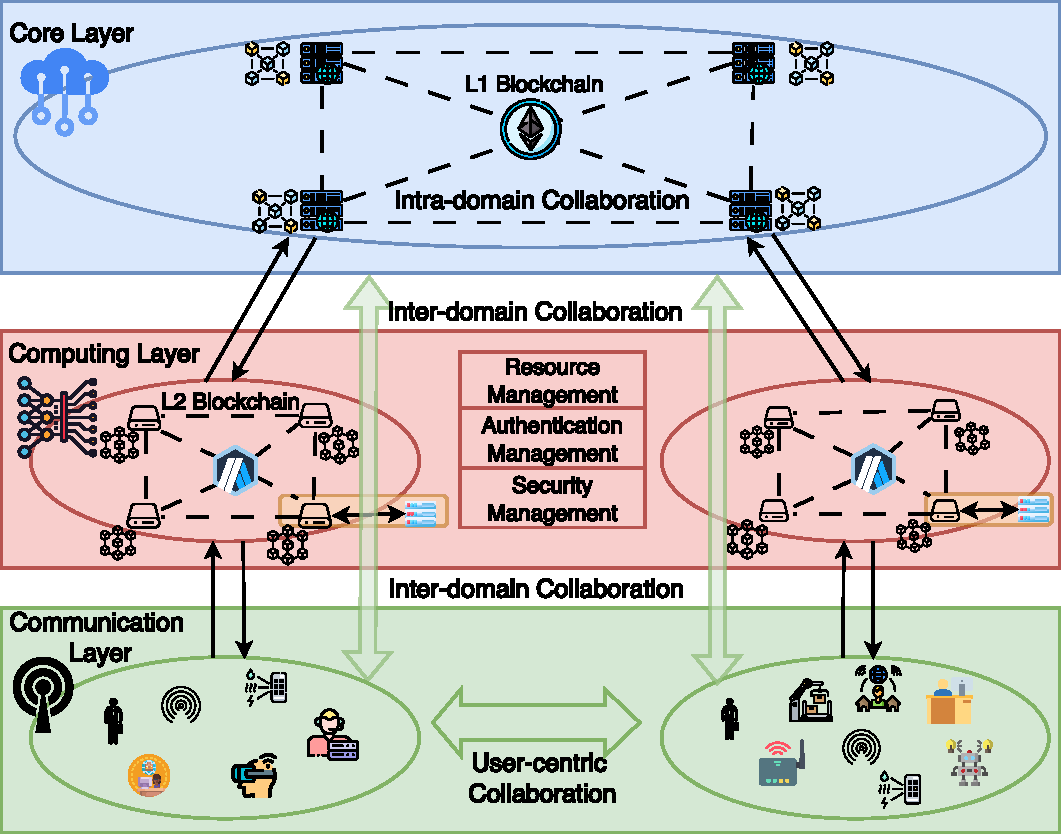
\includegraphics[width=\linewidth]{collaborate.pdf}
\caption{Proposed blockchain-based collaborative DeAI framework.}
\label{fig:collaborate}
\end{figure}



\subsection{Collaborative AI Development}
Collaborative AI in decentralized environments refers to scenarios where multiple independently operated systems or agents work together to solve complex tasks without relying on a central authority. Fig.~\ref{fig:collaborate} illustrates a blockchain-based collaborative DeAI framework in which decentralized core, computation, and communication layers coordinate resource allocation, security management, and authentication across L1 (for example, Ethereum) and L2 (for example, Arbitrum) blockchains, as well as user nodes. This multi-layered architecture supports inter-domain and intra-domain cooperation to achieve secure AI-enhanced computation and user-centric customization within a distributed network. Within this framework, collaborative AI development is formulated as a multi-agent learning problem where heterogeneous agents interact over a shared blockchain-based substrate. These agents include data-holding edge devices, service providers, model owners, relay nodes, and verifiers that participate in different parts of the workflow. Coordination follows local policies and protocol rules that govern task discovery, resource negotiation, and model-update scheduling across L1 and L2 networks, consistent with distributed negotiation and task-allocation mechanisms in multi-agent systems research~\cite{dorri2018multi,karim2025ai}. 

Several deployed systems exhibit this collaborative pattern across diverse domains. In industrial cyber-physical systems, DeAI frameworks integrate FL, blockchain, and generative adversarial networks so that local agents train intrusion-detection models on IIoT or edge-cloud telemetry under local differential privacy and then contribute distilled parameters to a global detector through decentralized federated distillation, while a Hyperledger Fabric component applies performance-weighted aggregation based on Quality-of-Service (QoS) requirements~\cite{liang2024enhanced,canonico2023industrial}. Digital twin-based IIoT monitoring and DeAI-enabled security services follow a similar structure: each agent refines a detection or control policy under domain-specific constraints and shares only model updates or alerts with the consortium. PoI platforms and relay-mining-based LLM inference networks extend this paradigm by assigning verifier roles to dedicated agents that validate model execution, usage records, and claimed performance before rewards are issued~\cite{bhat2023sakshi}. Across these designs, learning agents generate local decisions that feed higher-level aggregation logic encoded in smart contracts or consensus mechanisms, while verifier agents assess model updates, task completion, and cross-chain state transitions. Smart contracts encode matching rules and staking conditions to ensure predictable behavior without a central coordinator. Within this framework, learning agents generate local decisions that feed into higher-level logic, while verification agents audit these contributions to enforce correctness. While these architectures prove that decentralized multi-agent AI is feasible, current evaluations are often limited by resource constraints and have not yet been tested at the massive scale expected for future intelligence networks.



\subsection{Integration with Web3}
The integration of DeAI with Web3 significantly enhances the capabilities of dApps and DeFi platforms~\cite{cao2022decentralized,ray2023web3}. This integration broadens user engagement by enabling interactions from a diverse range of users and edge devices. As a result, Web3 platforms offer personalized services to a larger audience, thereby improving scalability and user experience~\cite{kersic2024review}. In addition, DeAI elevates the security and privacy of Web3 by incorporating advanced techniques such as FL, differential privacy, and homomorphic encryption~\cite{huang2024web3}. These techniques safeguard user data and interactions during P2P communication, and financial services to ensure confidentiality and protection against malicious activities. DeAI also plays a crucial role in enabling efficient, energy-sensitive, and trustworthy edge-cloud networking and computing. Such capabilities ensure that Web3 applications operate smoothly with low latency and high reliability in the decentralized ecosystem. DeAI further supports the creation of intelligent, adaptive, and personalized services within Web3. These services, which can incorporate immersive capabilities and virtual-physical interactions, enrich the user experience. Furthermore, DeAI fosters innovation and user participation by supporting the toolkits for Web3~\cite{allen2023web3}. These toolkits enable features such as end-user programming, interactive interfaces, and workflow management, thereby ensuring the robust development, management, and security of Web3 applications.

Olshansky et al.~\cite{olshansky2024decentralized} integrate LLM with remote procedure call (RPC) infrastructure in POKT Network\footnote{\url{https://www.pokt.network/}} to address the issues of limited experimentation, unsustainable business models, and unequal access in DeAI stack. POKT Network is a Web3-based framework that provides scalable and cost-effective RPC services across multiple blockchains. The authors utilize a relay mining algorithm that ensures transparent and verifiable request processing. They implement vertical decoupling strategies that separate system components to optimize operational efficiency, while simultaneously integrating decentralized storage and computational networks to strengthen the overall Web3 ecosystem's infrastructure. Although the solution demonstrates scalability for blockchain RPC requests, scaling the AI inference in high-end models will require modifications to the GPUs, which is not discussed briefly.

\subsection{Insights}
Collaborative learning mesh allows autonomous AI agents to participate in distributed tasks, while preserving fault tolerance, data privacy, and model integrity. The convergence of FL with blockchain consensus mechanisms establishes a secure workflow environment. In this environment, distributed validation verifies AI model integrity. Cross-chain AI collaboration is thus enabled while individual data sovereignty is preserved. At the same time, collective intelligence development is supported across heterogeneous decentralized networks.

\section{Generative Augmentation for User-centric Governance} \label{sec:genai}
This section explores GenAI as a generative augmentation framework that enhances user-centric governance in decentralized systems through intelligent content generation, automated security analysis, and adaptive user interfaces. We examine how GenAI transforms traditional governance mechanisms by providing automated vulnerability detection, real-time fraud prevention, intelligent contract analysis, and personalized user experiences that adapt to individual preferences and security requirements.


	
\subsection{Decentralized Governance and Human-Centered Oversight}
Decentralized governance in Web3 and DeAI systems extends beyond token voting or on-chain configuration changes. It defines how decisions about data usage, model deployment, and protocol evolution become visible to stakeholders and how responsibility for those decisions is assigned. In generative augmentation settings, governance also determines how GenAI services record their actions and expose explanations for users and auditors. Transparency arises when ledgers maintain append-only logs of transactions, model life cycles, and governance actions that capture commitments to training data sources, model versions, and relevant prompts and outputs without exposing raw records. System such as Zcash\footnote{\url{https://z.cash/}} shows that consensus-level transparency can coexist with protected transaction details through ZKPs, while the Oasis protocol demonstrates that secure multi-party computation and confidential execution can hide sensitive model training data from other participants. These designs indicate that transparency does not require full public disclosure of all data. Instead, verifiable commitments and cryptographic proofs allow external parties to check that agreed rules were followed, which supports trust and reliability while technical mechanisms preserve confidentiality.

Accountability and human-centered oversight complete this governance picture. Platforms such as SingularityNET\footnote{\url{https://singularitynet.io/}} apply community-driven control and fairness-constrained FL in AI marketplaces so that training processes align with shared ethical standards. Ocean Protocol\footnote{\url{https://oceanprotocol.com/}} keeps ownership of data with individual providers and grants controlled access through data tokens, which links data usage, compensation, and responsibility for misuse. Gitcoin\footnote{\url{https://www.gitcoin.co/}} uses quadratic funding and voting to balance the influence of large and small contributors when allocating resources to public goods, reducing the risk that a small group captures decision-making. In user-centric governance scenarios, GenAI components can summarize long on-chain histories, compare alternative proposals, and simulate potential outcomes in natural language so that human committees or token-holder assemblies can evaluate trade-offs more effectively. However, the final authority over policy updates, model approvals, and emergency interventions remains with human decision-makers who can incorporate contextual knowledge, value judgments, and off-chain information that are not fully represented in ledger data. This division of labor, where transparent records and accountable mechanisms are combined with human-centered oversight, underpins trust and reliability in decentralized governance for generative systems.



\subsection{Enhanced Blockchain Efficiency}
GenAI can optimize various aspects of blockchain, improving overall efficiency and performance. By utilizing advanced AI algorithms, GenAI can predict network congestion and optimize transaction processing times. Additionally, GenAI can help in designing more efficient consensus mechanisms, thereby enhancing the scalability and speed of blockchain networks. For example, Nguyen et al.~\cite{nguyen2024generative} investigate the potential of GenAI to address inherent challenges in blockchain, such as scalability, security, privacy, and interoperability. The authors utilize a Generative Diffusion Model (GDM) to demonstrate how GenAI can significantly optimize blockchain network performance metrics compared to traditional AI methods. Their findings suggest that GenAI leads to faster convergence, increased rewards, and improved throughput and latency. However, there are some limitations worth noting. The study's reliance on a single case study limits the generalizability of the results. Additionally, the paper does not comprehensively address the computational demands and scalability challenges associated with implementing GenAI in blockchains. Furthermore, a thorough investigation into the security risks introduced by such integrations is not included, which raises concerns about the feasibility of such an optimized blockchain framework in terms of real-world applicability. On the other hand, SmartLLM~\cite{xu2023smartllm} proposes a middleware that functions as the oracle to ensure secure, tamper-proof, and verifiable communication between the smart contracts and LLMs. It also allows the processing of complex and unstructured data by integrating NLP capabilities into smart contracts, which was previously beyond the scope of blockchain applications. While the system is designed to be trustless, it relies on the assumption that the middleware and the LLMs are secure and free from manipulation, which does not always align with the practical and evolving nature of the blockchain ecosystem.


\begin{figure*}[!t]
\centering
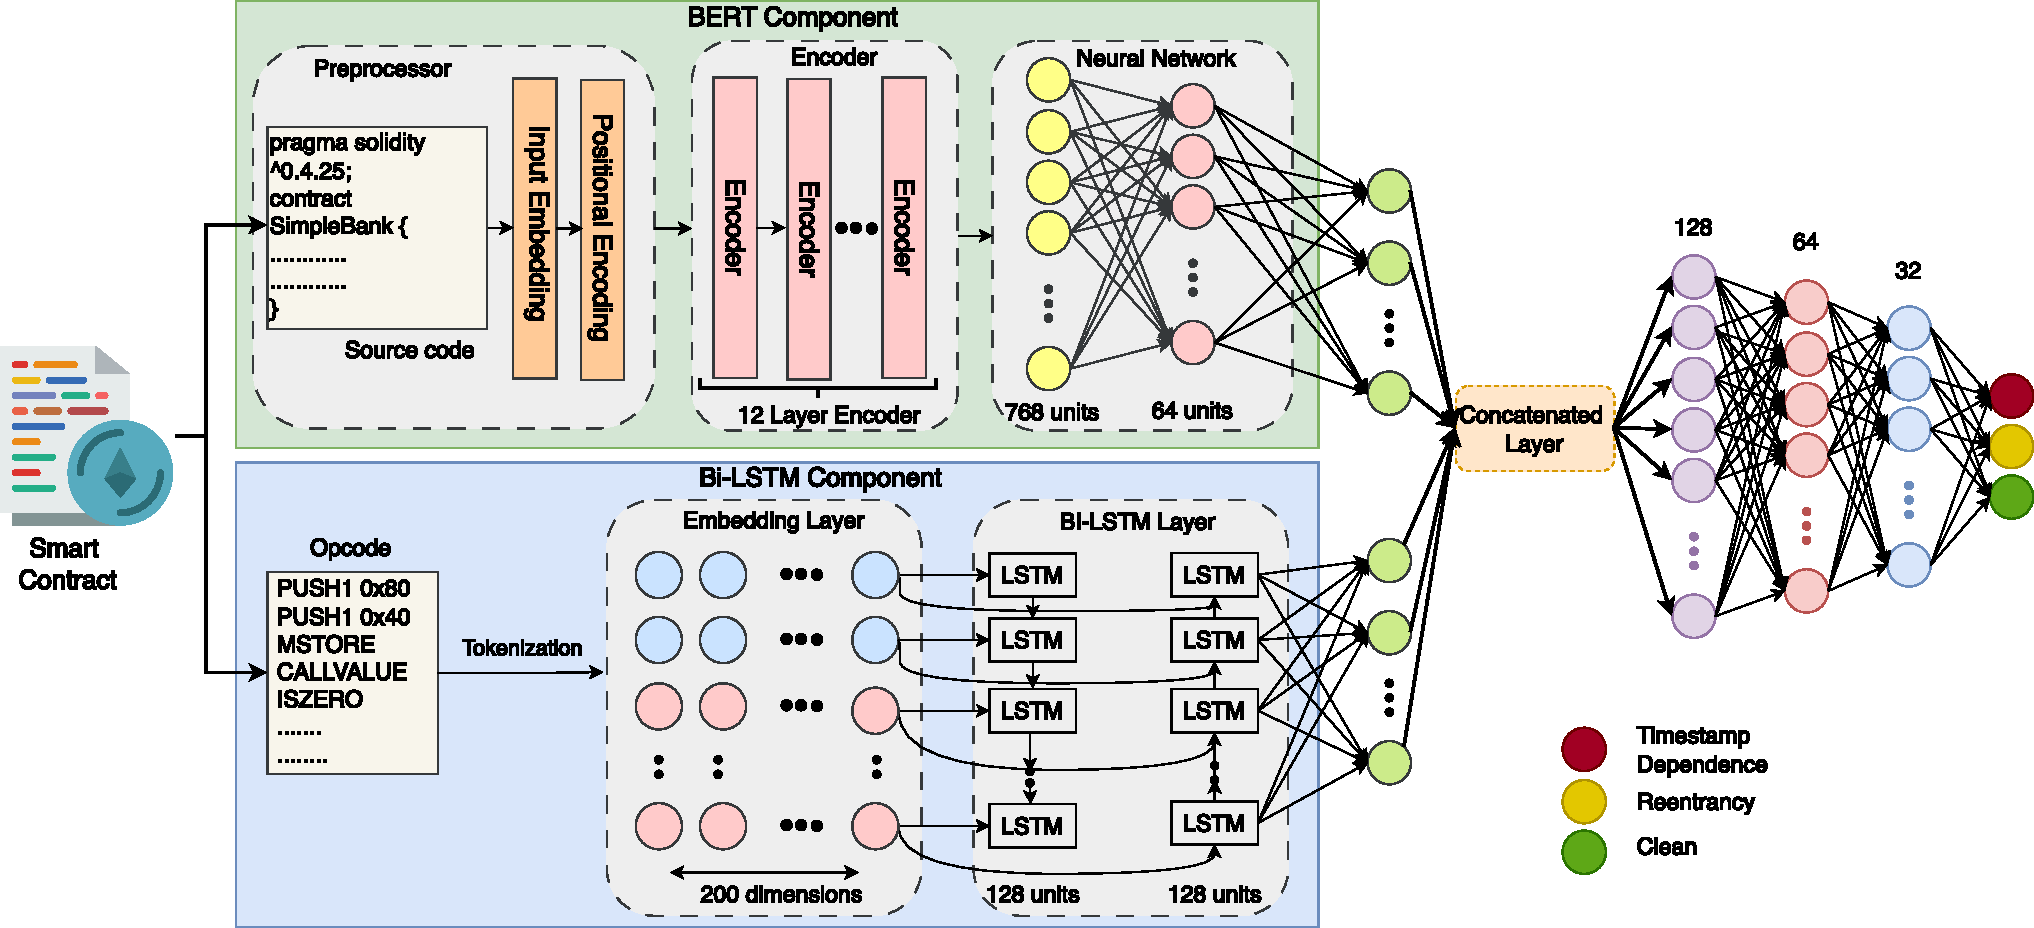
\includegraphics[width=0.80\linewidth]{contract.pdf}
\caption{GenAI-based smart contract vulnerability detection.}
\label{fig:smart}
\end{figure*}

\subsection{Smart Contract Vulnerability Detection}
GenAI-based smart contract vulnerability detection uses large pre-trained language or code models (e.g., BERT, CodeBERT, GPT-style LLMs) to learn semantic representations of contract source code or bytecode in order to automatically predict the presence and type of security flaws. Figure~\ref{fig:smart} illustrates a representative multimodal GenAI architecture designed to capture both the semantics and the execution logic of a contract. This framework operates through a dual-stream process. The upper stream processes the raw \emph{Source Code} to capture high-level logic: it utilizes a preprocessor to handle Solidity syntax, followed by input and positional embeddings, where a Transformer-based encoder (e.g., a BERT component) extracts deep semantic dependencies to interpret the programmer's intent. Simultaneously, the lower stream analyzes the compiled \emph{Opcode} using Bi-LSTM networks to capture the sequential dependencies of the machine-level execution flow. These distinct feature sets are then fused via a concatenated layer, facilitating the detection of vulnerabilities such as reentrancy, integer overflow or underflow, timestamp dependence, and insecure access control. Here, we discuss representative solutions that leverage these models to highlight their capabilities, application scopes, and the remaining challenges in this domain. Table~\ref{tab:genai-sc} provides a comparative overview of GenAI-based smart contract vulnerability detection solutions, including vulnerabilities addressed, methods, GenAI models employed, datasets, performance metrics, and key observations. 

In the realm of semantic representation, early GenAI adaptions primarily utilized encoder-based models to enhance code comprehension. A prominent example is SCVulBERT~\cite{zeng2023high}, which employs a BERT-based approach to address smart contract vulnerability detection challenges, including reentrancy, timestamp manipulation, and delegate call issues.
%
The model utilizes a specialized tokenizer for efficient code representation, leverages transfer learning~\cite{zhuang2020comprehensive} to address data scarcity, and extracts semantic features from code using BERT to enhance vulnerability comprehension. While SCVulBERT demonstrates improved accuracy, precision, recall, and F1-score in vulnerability detection, the computational intensity and reliance on high-quality pre-trained models remain notable limitations.

In regards to multimodal deep learning, Trinh et al.~\cite{trinh2023multimodal} leverage features from both source code and opcodes to improve detection accuracy. The authors integrate BERT and BiLSTM~\cite{bin2016bidirectional} for processing source code and opcode analysis, respectively. They also utilize two datasets to demonstrate significant performance improvements across metrics such as accuracy and F1-score, while considering vulnerabilities such as reentrancy, arithmetic, and timestamp dependence. Despite its promising results, the research is limited by the diversity of the datasets and the model's generalizability to other blockchain platforms. Likewise, Lian et al.~\cite{lian2024universal} propose a multimodal fusion learning approach that integrates features extracted from smart contracts. Their methodology incorporates advanced models such as EfficientNet~\cite{tan2019efficientnet}, BiLSTM, and Transformers~\cite{vaswani2017attention} to enhance the feature representation. The authors leverage the SmartBugs-Wild dataset~\cite{web-smartbug-dataset}, which comprises over 40,000 smart contract samples, to validate their methodology through extensive experiments. Despite its strengths, the framework encounters limitations such as computational intensity, potential overfitting, and the need for broader applicability across different blockchain platforms. Furthermore, Yiting et al.~\cite{yiting2024automated} employ a pre-trained BERT model to preprocess smart contract code by standardizing variable names and substituting symbols with natural language to facilitate feature extraction. Their research focuses on four prevalent vulnerabilities: integer overflow, reentrancy, timestamp manipulation, and access control issues. The method excels in handling both large and small datasets for real-time applications. However, the static analysis approach lacks the capability to simulate smart contract execution, which limits its ability to detect runtime-specific issues and dynamic interactions between contracts.

Beyond detection, researchers have also explored generative models for auxiliary tasks. For example, SCCLLM~\cite{zhao2024automatic} leverages LLMs and in-context learning for automatic smart contract comment generation. The process consists of three novel phases: (1) a customized demonstration selection phase that uses CodeBERT~\cite{feng2020codebert} to retrieve semantically, syntactically, and lexically similar code snippets; (2) an in-context learning phase that constructs tailored prompts for the LLM; and (3) a final inference phase that generates comments using ChatGPT's API, thereby circumventing the need for extensive model training. Despite its advantages, the approach has several limitations. For instance, it depends on the quality of demonstration examples and encounters difficulties in generating comments for complex code snippets. Moreover, potential scalability issues arise from its dependence on LLM APIs. Another method named Vulnerability-constrained Decoding~\cite{storhaug2023efficient} uses LLMs to address the issue of vulnerabilities in auto-completed smart contract code. This involves fine-tuning the GPT-J-6B model\footnote{\url{https://huggingface.co/EleutherAI/gpt-j-6b/}} on a large dataset of Ethereum smart contracts. Vulnerable code segments are labeled to fine-tune the model in order to avoid insecure code generation. This fine-tuning process restricts the model from generating labeled vulnerabilities by adjusting the probability of those outputs during the decoding phase. It also prevents the generation of vulnerable code in about 67\% of cases, while achieving a high BLEU score of 0.557. However, there are potential trade-offs between code completeness and security due to the reliance on labeled data.

In regard to detecting multiple vulnerabilities in smart contracts, Tong et al.~\cite{tong2024enhancing} incorporate a BERT-based language model with word embedding techniques (e.g., TF-IDF~\cite{aizawa2003information}, Word2Vec~\cite{church2017word2vec}). They introduce a neural network architecture to reduce misclassification by adding a neuron that identifies uncertain predictions. In addition, they develop a hybrid model for benchmarking that includes Ethereum smart contract datasets with multiple vulnerabilities such as outdated versions, frozen ether, time dependence, and delegatecall injection. However, their solution struggles with detecting outdated version vulnerabilities due to the exclusion of critical information in bytecode sequences longer than 512 tokens. GPTScan~\cite{sun2024gptscan} combines GPT models with static analysis to detect vulnerabilities in smart contracts. It breaks down each type of vulnerability logic into scenarios and properties, which describe the code functionality and vulnerable attributes. The tool takes an average of 14.39 seconds and \$0.01 to scan per thousand lines of Solidity code with a 90\% precision for token contracts, 57.14\% for large projects, and 70\% recall rates in terms of detecting ground-truth logic vulnerabilities. However, the effectiveness relies heavily on predefined scenarios and properties. Additionally, it demonstrated a drop in precision when analyzing large projects with complex logic.

On the other hand, TrapFormer~\cite{gu2023trap}, a transformer-based model, has been proposed to detect trap contracts (e.g., Ponzi schemes and honeypots) on the Ethereum platform. The model leverages opcode segmentation, a densely connected transformer, and adaptive data augmentation to process the ultra-long sequences typical of smart contract opcodes while mitigating the risk of overfitting due to category imbalance. The solution achieves an F1-score of 0.984 and 0.965 in terms of detecting honeypots and Ponzi schemes, respectively. However, there are some notable limitations. First, the adaptive data augmentation method relies heavily on synthetic data generation to balance categories. Second, the computational complexity of the transformer model remains high, which limits the model's scalability in environments with constrained computational resources.


\begin{table*}[!t]
\centering
\caption{Comparison of literature on GenAI-based smart contract vulnerability detection.}
\label{tab:genai-sc}
\footnotesize
\selectfont
\setlength\tabcolsep{0.6pt}
\begin{tabularx}{\linewidth}{
>{\hsize=0.05\hsize}Z
>{\hsize=0.15\hsize}Z
>{\hsize=0.20\hsize}Z
>{\hsize=0.15\hsize}Z
>{\hsize=0.13\hsize}Z
>{\hsize=0.12\hsize}Z
>{\hsize=0.20\hsize}Y}
\toprule 
\textbf{Ref.} & \textbf{Vulnerability} & \textbf{Method} & \textbf{GenAI Model} & \textbf{Dataset} & \textbf{Metrics} & \multicolumn{1}{c}{\textbf{Remarks}} \\\midrule

~\cite{trinh2023multimodal} & \makecell[c]{Generic smart \\contract} & \makecell[c]{Multimodal learning \\of source code \\attributes} & BERT, Bi-LSTM & Smartbugs Wild, SolidiFI~\cite{ghaleb2020effective} & \makecell[c]{AC,PR,\\RE,F1} & \makecell[l]{i) Execution traces are not\\ considered\\ii) Interpretability issue\\ due to multimodal model} \\\hline

~\cite{zeng2023high} & \makecell[c]{Reentrancy, \\timestamp, \\and delegate call} & \makecell[c]{Contract feature \\extraction} & BERT & \makecell[c]{Smart-Contract\\Dataset} & \makecell[c]{AC,PR, \\RE,F1} & \makecell[l]{i) Utilize transfer learning\\ for accuracy\\ii) Struggle with large\\ sized contracts} \\\hline 

~\cite{lian2024universal} & \makecell[c]{Reentrancy, DoS, \\integer overflow} & Multimodal learning from source code, bytecode, and opcode & EfficientNet, BiLSTM, Transformer & SmartBugs Wild~\cite{web-smartbug-wild} & \makecell[c]{AC,PR,\\RE,F1} & \makecell[l]{i) Require larger contracts\\ii) Data processing needs\\ optimization} \\\hline 

~\cite{yiting2024automated} & Reentrancy, timestamp, integer overflow & Pre-process and symbol substitution & BERT & Public dataset & \makecell[c]{AC,PR,\\RE,F1,\\FPR,FNR} & \makecell[l]{i) Dataset size is limited\\ii) Need large dataset for\\ accuracy} \\\hline 

~\cite{zhao2024automatic} & Generic & \makecell[c]{In-context learning,\\ semantic vector\\ extraction} & GPT-3.5-turbo & Etherscan & \makecell[c]{BLEU,\\Rouge,\\Gouge} & \makecell[l]{i) Lexical retrieval\\ for in-context learning\\ii) Improve comment\\ generation by 7-17\% } \\\hline

~\cite{storhaug2023efficient} & \makecell[c]{Auto-completed \\code} & \makecell[c]{Vulnerability \\constraint \\decoding} & GPT-J & Hu et al.~\cite{hu2023smart} & CrystalBLEU~\cite{eghbali2022crystalbleu} & \makecell[l]{i) Additional testing for\\ non-Ethereum\\ii) Reduce 67\% \\vulnerabilities} \\\hline 

~\cite{tong2024enhancing} & \makecell[c]{Ineffective word \\embedding} & \makecell[c]{Reduce \\misclassification \\rate} & BERT & Ethereum ETL & \makecell[c]{PR,RE,\\F1,EMR} & \makecell[l]{i) High F1-score and low\\ execution time\\ii) Struggle with large\\ dataset} \\\hline 

~\cite{sun2024gptscan} & Smart contract logic & Static and dynamic analysis & GPT-3.5-turbo & \makecell[c]{Top200,\\Web3Bugs,\\DefiHacks} & \makecell[c]{PR,RE,\\FPR,FNR} & \makecell[l]{i) Rely on ANTLR,\\ crytic-compiler~\cite{web-crytic}\\ii) Validate GPT output} \\\hline 

~\cite{gu2023trap} & \makecell[c]{Ponzi schemes, \\honeypots} & \makecell[c]{Adaptive data \\augmentation} & Transformer & \makecell[c]{Ethereum \\multi-trap \\contract} & \makecell[c]{AC,PR,\\RE,F1} & \makecell[l]{i) Focus on Ethereum\\ii) Outperform CNN,\\LSTM,GRU} \\\bottomrule 

\end{tabularx}
\begin{tablenotes}
\item \textbf{AC}=Accuracy; \textbf{PR}=Precision; \textbf{RE}=Recall; \textbf{F1}=F1-Score; \textbf{FPR}=False Positive Rate; \textbf{FNR}=False Negative Rate; \textbf{EMR}=Exact Match Ratio.
\end{tablenotes}
\end{table*}

\subsection{Fraud Detection and Threat Hunting}
GenAI enhances the security of blockchain by providing advanced fraud detection mechanisms~\cite{zhou2024artemis,hu2023bert4eth,zkik2024cyber,rawlins2023predicting,rabieinejad2023generative}. By analyzing patterns and anomalies in transaction data, GenAI identifies potentially fraudulent activities with high accuracy. This is essential for maintaining the integrity and trustworthiness of blockchain networks. In terms of Web3, GenAI-driven security measures protect decentralized applications from malicious attacks to ensure a safer user environment. For example, Zhou et al.~\cite{zhou2024artemis} introduce ARTEMIS, a system designed to detect airdrop hunters who exploit token distribution through manipulative practices in NFT markets. ARTEMIS utilizes GenAI by employing pre-trained Transformer models, such as BERT and ViT, to extract multimodal features from NFTs. This approach enables the system to capture the complex visual and textual data inherent in these assets. ARTEMIS identifies anomalous behaviors through graph neural networks (GNNs), which model NFT transaction interactions, and incorporates market manipulation indicators, including Benford's Law, to detect irregularities in transaction prices.

Detecting fraudulent activity on Ethereum requires robust models capable of handling repetitive, skewed, and heterogeneous transaction data. BERT4ETH~\cite{hu2023bert4eth} introduces a pre-trained transformer model that overcomes the limitations of traditional graph-based methods by effectively capturing dynamic sequential patterns in blockchain transactions. Through techniques like transaction de-duplication, high masking ratios, and frequency-aware negative sampling, BERT4ETH reduces label leakage while preserving the uniqueness of account representations. In evaluations, this model demonstrates significant performance gains, notably achieving a 21.61\% improvement in the F1 score for phishing detection, marking a substantial advance over prior methods.

In regard to improving cyber resilience on online retail platforms, Zkik et al.~\cite{zkik2024cyber} leverage GANs, explainable deep learning (XDL)~\cite{la2023state}, and a blockchain-based consensus protocol to perform intelligent fraud detection. GANs are employed to simulate various forms of cyber-attacks, such as DDoS attacks, injection attacks, and advanced persistent threats. Additionally, XDL contributes to identifying and highlighting the specific features within the data that are most relevant to fraudulent activities. Meanwhile, the consensus protocol includes a weighted voting system and a rotation mechanism for distributing authoritative responsibilities among nodes. The experimental validation is conducted in a controlled environment, which does not fully capture the complexity and variety of cyber threats faced in real-world scenarios. Furthermore, VecGAN~\cite{rawlins2023predicting} detects fraudulent transactions in IoT-based blockchain systems using a lightweight GAN. The solution is integrated with Bayesian feedback alignment to enhance training stability and computational efficiency in resource-constrained environments. It replaces existing PoW consensus by offering a combined approach of both data augmentation and subsequent classification. Experimental results show that VecGAN reduces computational intensity and increases block throughput by 50\% while improving fraud detection accuracy by up to 3\%. Although BFA reduces computational overhead, it still requires significant memory resources, which is a limiting factor for resource-constrained IoT devices.

On the other hand, ZipZap~\cite{hu2024zipzap} enhances the training efficiency of LLMs for performing large-scale fraud detection in Ethereum. It features an asymmetric training paradigm, which accelerates pre-training by using transaction dropping and cross-layer parameter sharing. Additionally, it introduces a frequency-aware compression method that reduces the model size to 7.5\%. This method also reduces the parameter count of the original LM by 92\%, with minimal impact on performance. Nevertheless, ZipZap's training approach introduces biases that lead to overfitting during the pre-training phase. Furthermore, the framework is limited to the context of BERT and Ethereum. 
%
Moreover, Rabieinejad et al.~\cite{rabieinejad2023generative} propose an enhancement to Ethereum by employing GANs with BiLSTM to detect threats in DeFi and dApps. A two-phase model is developed to address the increasing threat of sophisticated attacks such as adversarial attacks, scamming, phishing attacks, and low-rate DDoS attacks. In the first step, a Conditional GAN (CTGAN) is employed to generate realistic attack-oriented transactions that resemble genuine Ethereum transactions. In the second step, these transactions are used to train a BiLSTM to accurately detect and identify attacks with a high accuracy of 99.98\%. However, there are some limitations regarding the computational complexity of the GAN-BiLSTM model, scalability issues in high-transaction environments, reliance on data quality, and potential vulnerabilities to data poisoning attacks.

\begin{figure}[!t]
\centering
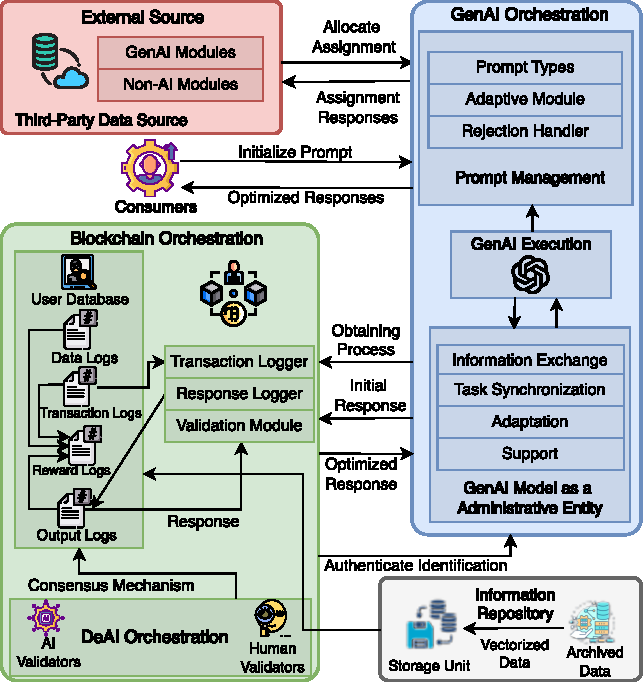
\includegraphics[width=0.90\linewidth]{governance.pdf}
\caption{GenAI extension on the top of blockchain-based governance model.}
\label{fig:governance}
\end{figure}

\subsection{GenAI-enabled Web3}
Integrating GenAI with Web3 involves establishing interoperability standards and protocols that enable seamless interaction between AI models and decentralized platforms. Web3 supports decentralized AI training environments, which allows generative models to be trained collaboratively without relying on centralized data repositories. This integration not only enhances the capabilities of GenAI but also ensures that the generated content is secure, verifiable, and resistant to manipulation. For instance, Duan et al.~\cite{duan2023metacube} introduce MetaCube, a novel user-generated content editor that leverages GenAI to enhance content creation within the Web3 metaverse. To address the challenges of content uniqueness and 3D model complexity, the authors propose a combination of voxel-based modeling and GANs. The innovative 3D Crypto-dropout technique integrates blockchain-based cryptographic information to produce unique and detailed 3D models. This approach ensures distinct ownership of each content piece, democratizes digital asset creation, and facilitates a more accessible and secure creator economy within the decentralized Web3 ecosystem.

As for decentralized decision-making, the integration of GenAI and Web3 strengthens autonomy, transparency, and scalability in governance processes. Fig.~\ref{fig:governance} illustrates a representative GenAI- and blockchain-based governance framework, in which GenAI supports governance by coordinating decentralized data management and task execution. In parallel, a blockchain-based operational layer records and verifies identity, billing, and incentive mechanisms through smart contracts and auditable feedback loops. Building on this paradigm, Zhang et al.~\cite{zhang2024decoding} investigate the convergence of large language models and Web3-based decentralized autonomous organizations to enable decentralized decision-making and address misinformation. Their study demonstrates how LLMs improve the governance and coordination of decentralized activities by analyzing large-scale public data and identifying dissemination patterns. DAOs are deployed on blockchain infrastructures to enhance transparency and ensure information authenticity. Furthermore, the authors illustrate how GenAI techniques reinforce the reliability and operational efficiency of Web3 ecosystems. Despite its novelty, the DAO-based approach to disinformation mitigation remains primarily conceptual and lacks validation in real-world deployments. 

On other hand, MERLIN~\cite{costa2023studying} is a multimodal deep learning framework that predicts the selling price categories of NFTs using LMMs. It employs a two-stage methodology, where the first stage fine-tunes pre-trained language and visual models to generate dense representations of NFT data. Consequently, the second stage employs a graph attention network (GAT) to enhance contextual awareness through similarity-based aggregation. MERLIN achieves an accuracy of approximately 77.3\%, a win rate of 92.6\%, a low loss rate of 7.4\%, and a cautiousness metric of 0.688. However, there are also some limitations, including dependency on the quality of the training dataset, social media influence, and lack of temporal analysis (e.g., re-sale times of NFTs). Another framework named EKILA~\cite{balan2023ekila} addresses the provenance and attribution issues of GenAI art in the Web3 ecosystem. The framework leverages NFTs and blockchain to create a decentralized system where creators retain control over their works. EKILA implements an automated royalty mechanism to facilitate cryptocurrency payments to creators based on their contributions. This connects ownership, rights, and attribution to ensure the recognition and compensation of creativity in rapidly evolving digital art. As for limitations, the scalability of managing large datasets and complex NFT interactions poses challenges that can impact the effectiveness of EKILA in real-world applications.

\subsection{Content Generation and Data Augmentation}
GenAI-driven content generation and data augmentation are critical for advancing the usability and scalability of blockchain, Web3, and DeAI systems. As illustrated in Fig.~\ref{fig:aigc}, the lifecycle of AIGC products typically spans three critical phases: Generation, Distribution, and Trading. Phase 1 involves the interaction between users and edge service providers to generate content; Phase 2 highlights the distribution risks, where malicious actors may exploit platforms to tamper with or plagiarize content; and Phase 3 focuses on the secure verification required for legitimate trading. Addressing these lifecycle challenges, Liu et al.~\cite{liu2024blockchainempowered} propose a blockchain-empowered framework to enhance the management of AIGC products in edge networks. The authors address key challenges related to security, trustworthiness, and efficiency in content generation using GenAI. The framework incorporates a reputation-based selection of edge service providers by utilizing multi-weight subjective logic to optimize the assignment of content generation tasks based on service quality. Furthermore, an on-chain incentive mechanism guarantees the secure and legitimate exchange of funds and ownership in order to promote the efficient circulation of AIGC products. In the context of decentralized trading (Phase 3), MetaTrade~\cite{truong2024trust} manages secure and trust-free AIGC exchange within the metaverse. The framework tackles key issues such as trust, data security, and scalability by eliminating the need for intermediaries. It also employs multi-layer encryption and leverages decentralized storage. The integration of a reputation and rating system encourages honest participation and prevents malicious activities. To demonstrate superior cost efficiency and throughput performance, MetaTrade is implemented on Ethereum and Hyperledger Fabric blockchains. However, it faces limitations related to scalability, interoperability, regulatory compliance, and the integration of AI-based functions. These limitations impact its broader applicability in large-scale metaverse environments.

\begin{figure*}[!ht]
\centering
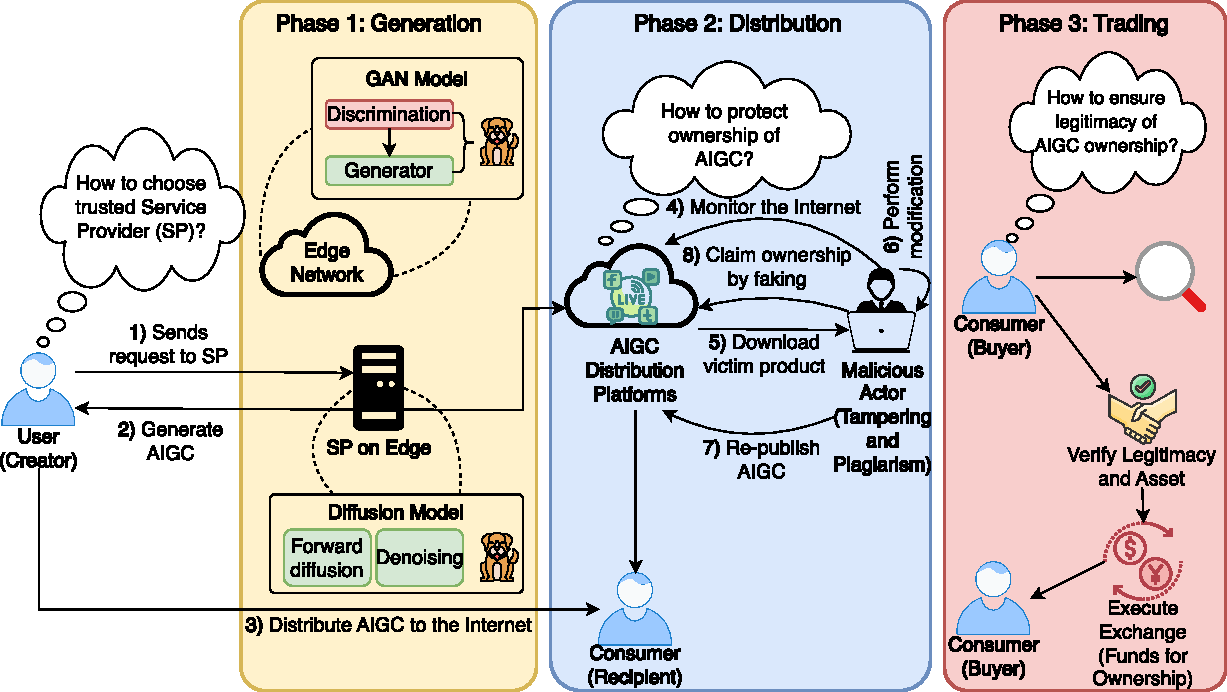
\includegraphics[width=0.70\linewidth]{aigc-v2.pdf}
\caption{Lifecycle management of AIGC products.}
\label{fig:aigc}
\end{figure*}

Data augmentation helps to expand the datasets used in the development and training of smart contract applications. This process is crucial for enhancing the effectiveness of ML models in areas such as vulnerability detection and automated contract analysis. GenAI enables the generation of synthetic data that mimics the properties of existing smart contracts. By employing advanced models, GenAI creates valid smart contract instances that not only enhance the quantity but also the diversity of data, leading to more robust ML models. For example, Hwang et al.~\cite{hwang2024cggnet} propose a novel approach called Compiler-Guided Generation Network (CGGNet). This specifically targets smart contract data augmentation. CGGNet uses a compiler as an oracle to ensure the validity of generated contracts and overcome the limitations of existing GAN-based methods~\cite{sharma2024generative,saad2024survey,lim2024future}. Additionally, CGGNet integrates Monte Carlo tree search to enhance the diversity of the generated contracts by generating millions of unique and valid smart contracts from a relatively small dataset.


\subsection{Generative Trustworthy Immersive Ecosystem}
A generative trustworthy immersive ecosystem denotes deployments where LLM-based agents operate with explicit guarantees for privacy, provenance, and economic accountability. Within the trust-to-augmentation framework in Section~\ref{sec:framework}, such an ecosystem spans all four layers: interaction and data capture at the edge, FL-based local adaptation, blockchain-coordinated trust and incentives, and agentic services that drive user-facing behavior in extended reality and Web3 applications~\cite{zhang2025industrial,zuo2025federated}. Our framework aggregates these requirements into the four-layer stack illustrated in Fig.~\ref{fig:trusted-immersive}. The interaction and data layer captures multimodal traces from virtual scenes, sensor streams, and natural-language exchanges while raw data remains on local devices or metaverse shards~\cite{zhang2025industrial}. The FL and local adaptation layer hosts frozen LLM backbones with lightweight trainable adapters on edge clients; clients conduct FL rounds over local interaction data and send encrypted model updates or gradients to aggregators without disclosing raw traces, supported by decentralized secure aggregation and blockchain-enhanced trust mechanisms~\cite{zuo2025federated,li2025dsafl}. The blockchain-based trust and coordination layer manages FL round registration, incentive distribution, and reputation through smart contracts, records cryptographic commitments to model versions in an immutable model registry, and enforces access policies for LLM and agentic services~\cite{zuo2025federated,liu2025polylink,luo2025weighted}. The LLM and agentic service layer builds on this trusted global model to deploy companion, moderation, and governance agents that operate inside metaverse applications and on-chain workflows; new interactions return to the data layer and trigger subsequent adaptation cycles~\cite{bandara2024generative,golam2025blind,liu2025polylink}.

\begin{figure*}[!t]
\centering
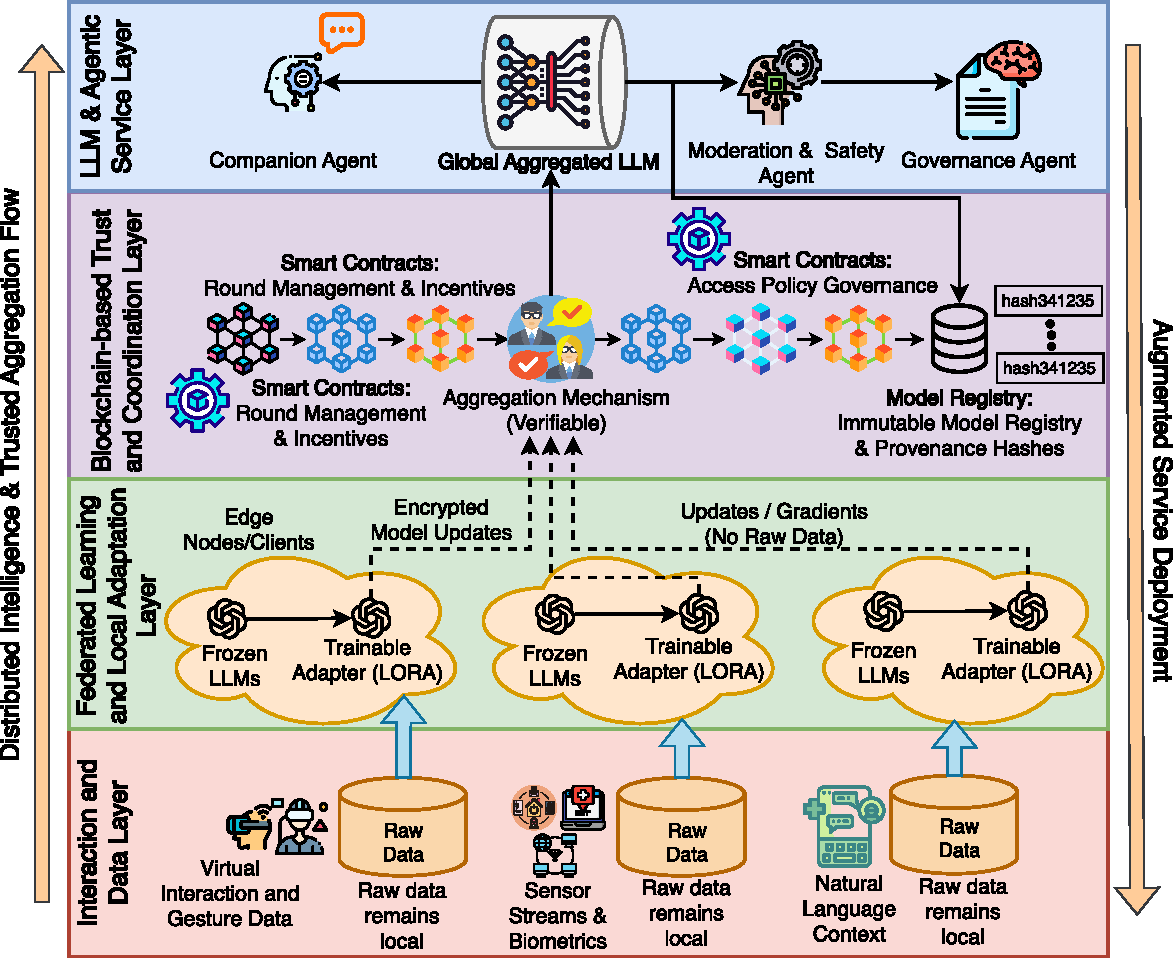
\includegraphics[width=0.60\linewidth]{llm-fl-bc-meta.pdf}
\caption{Illustration of a generative trustworthy immersive ecosystem.}
\label{fig:trusted-immersive}
\end{figure*}

Several recent studies instantiate individual components of this ecosystem and collectively motivate the need for a unifying architectural framework. Approaches targeting data sovereignty and model provenance, such as generative metaverse architectures, integrate FL with blockchain and NFT-based asset management to safeguard user data in extended-reality environments~\cite{bandara2024generative,zhang2025industrial}. Efforts emphasizing trust-layer coordination include blockchain-assisted digital-twin frameworks that couple tamper-evident telemetry with LLM-based cyber defence for industrial AIoT scenarios~\cite{golam2025blind}, as well as blockchain-anchored multi-LLM networks that employ weighted BFT consensus to coordinate model outputs for AIGC and metaverse governance~\cite{luo2025weighted}. At the agentic service layer, DeAI platforms such as PolyLink distribute LLM inference across geo-distributed edge devices and leverage blockchain-based incentives and trustless evaluation mechanisms to ensure inference integrity~\cite{liu2025polylink}.While these works highlight the complementary roles of FL and blockchain in LLM deployment, each addresses only a subset of the end-to-end system. In contrast, the proposed generative trustworthy immersive ecosystem offers a unifying architectural template that systematically organizes these fragmented solutions across all four layers and explicitly exposes the remaining integration challenges.



\subsection{Insights}
The integration of enhanced blockchain efficiency optimization, automated vulnerability detection, fraud prevention mechanisms, Web3 protocol enhancement, and data augmentation capabilities establishes GenAI as a comprehensive generative augmentation framework for user-centric governance. This transforms GenAI from a content creation tool into an intelligent governance layer that continuously monitors, analyzes, and improves decentralized systems through automated security analysis, synthetic data generation, and adaptive user interfaces. The convergence of LLMs with blockchain consensus mechanisms creates self-governing ecosystems capable of autonomous threat detection, intelligent contract analysis, and personalized user experiences that adapt to individual security requirements and preferences, fundamentally enabling user-centric governance in decentralized environments.

\begin{figure*}[!t]
\centering
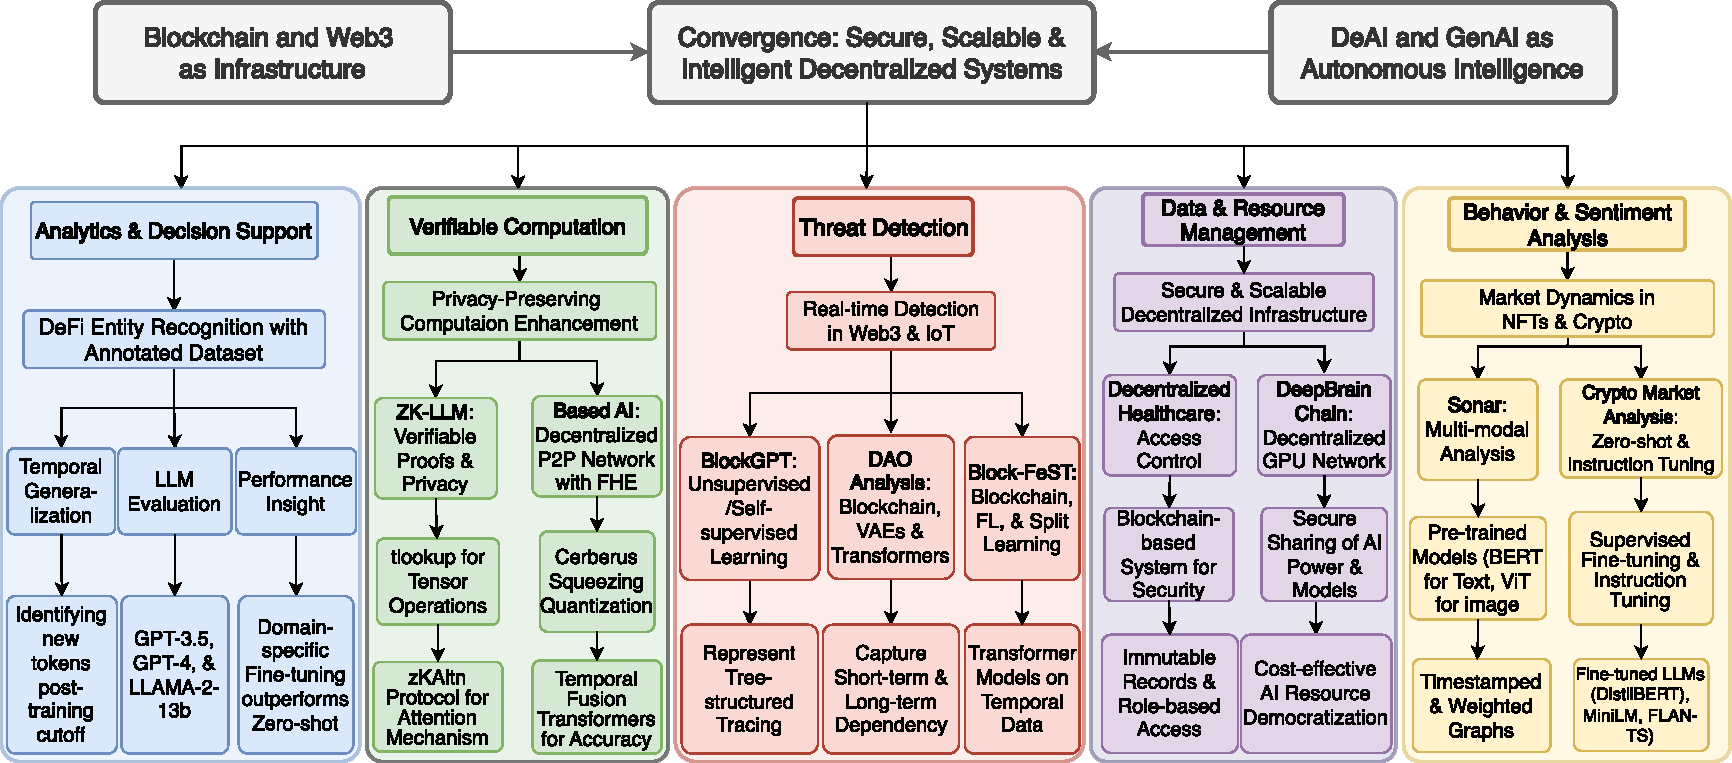
\includegraphics[width=\linewidth]{schematic.pdf}
\caption{Integrated application landscape for decentralized and generative intelligence.}
\label{fig:schematic}
\end{figure*}

\section{Applications and Use Cases} \label{sec:app}
In this section, we examine five representative application domains selected to demonstrate the practical implementation of the trust-to-augmentation framework layers proposed in Section~\ref{sec:framework}. These domains are chosen for their strategic significance in addressing critical challenges spanning financial transparency, privacy preservation, security assurance, and data-driven market intelligence. Figure~\ref{fig:schematic} presents a schematic taxonomy of this landscape, organizing these domains into distinct pillars supported by the convergence of blockchain and Web3 infrastructure with decentralized and generative intelligence. Within each domain pillar, the figure identifies specific operational tasks and representative systems, such as DeFi entity recognition, verifiable inference protocols, and real-time threat hunting models. A summary of these applications and use cases is provided in Table~\ref{tab:app}.

\subsection{DeFi Analytics and Decision Support}
DeFi offers a high-impact setting where decentralized and generative intelligence jointly influence security, market integrity, and user decision making. Blockchain execution and transparent ledgers provide an auditable substrate for financial actions, yet DeFi participants still face rapid protocol evolution, complex contract logic, and adversarial behaviors. DeAI supports collaborative risk sensing and threat detection across heterogeneous actors, while GenAI strengthens user-centric interaction through summarization, semantic parsing, and automated interpretation of on-chain and off-chain signals. Within this landscape, LLM-centric analytics and assistants improve the accessibility of DeFi interfaces and enhance the responsiveness of monitoring and compliance workflows.

In DeFi ecosystems, LLM-based semantic analytics support tasks such as entity recognition, protocol and product identification, and rapid interpretation of newly emerging tokens and applications. A recurring challenge is that DeFi terminology and entities evolve quickly, which exposes limitations in model knowledge after the training cutoff and motivates domain adaptation through few-shot prompting or fine-tuning. Pearlson et al.~\cite{pearlson2024evaluating} operationalize this setting by constructing an annotated Named Entity Recognition (NER) dataset with 7,338 labeled sentences covering cryptocurrencies, applications (or products), and programs. Their evaluation shows that models such as GPT-3.5 and GPT-4 recognize established entities reliably, whereas performance degrades on newly introduced DeFi entities unless domain-specific adaptation is applied through zero-shot, few-shot, or fine-tuning configurations.

\subsection{Privacy-Preserving Verifiable Computation}
The integration of large models has opened up new avenues for secure and privacy-preserving language processing applications. One particularly promising area of research is the combination of LLMs with ZKPs, which enables the validation of complex computations without revealing underlying sensitive information. By leveraging ZKPs, LLMs can be deployed in a wide range of scenarios that require robust security and privacy guarantees, such as secure language translation, and privacy-preserving sentiment analysis. For example, ZK-LLM~\cite{sun2024zkllm}, a ZKP scheme tailored specifically for LLMs, uses a combination of sum-check protocols, polynomial commitments, and lookup arguments to achieve zero-knowledge verifiability. ZK-LLM includes two novel ZKP protocols: \emph{tlookup} and \emph{zkAttn} protocol. The \emph{tlookup} protocol is designed to efficiently handle non-arithmetic tensor operations in deep learning through parallel computing, such as GPUs. This protocol adds no asymptotic overhead in memory complexity or runtime to ensure efficient operation without increasing computational or memory demands as the size of the tensors grows. Consequently, the~\emph{zkAttn} protocol is developed as a dedicated ZKP solution for the attention mechanism to ensure efficient and accurate zero-knowledge verification. Performance analysis demonstrates that ZK-LLM generates verifiable proofs for LLMs with up to 13 billion parameters in under 15 minutes, with compact proof sizes less than 200 KB. Despite these significant advancements, the approach faces limitations such as computational and memory overhead, error tolerance due to quantization, and challenges in scaling to the training phase.

Recent work explores privacy-preserving computation to protect both inputs and intermediate states during decentralized processing. For instance, BasedAI~\cite{wellington2024basedai} integrates homomorphic encryption~\cite{martins2017survey} with LLMs to ensure data privacy. It employs a quantization mechanism termed \textquote{Cerberus Squeezing} to convert standard LLMs into ZK-LLMs. This mechanism improves the efficiency of encrypted computation and enables miners to process and respond to encrypted queries without performing decryption. The network incentivizes participation through a token-based reward system and incorporates temporal fusion transformers to improve predictive accuracy and support consensus mechanisms. Potential applications and use cases of BasedAI include healthcare (as shown in Figure~\ref{fig:zk_llm_health}), financial trading, cybersecurity, anonymous search, and Bittensor subnets. These capabilities demonstrate BasedAI's ability to balance data security and computational demands within a decentralized architecture. Nevertheless, the system faces notable challenges related to scalability, technical complexity, and resource intensity, which remain critical barriers to large-scale adoption and real-world deployment.

\begin{figure}[ht!]
\centering
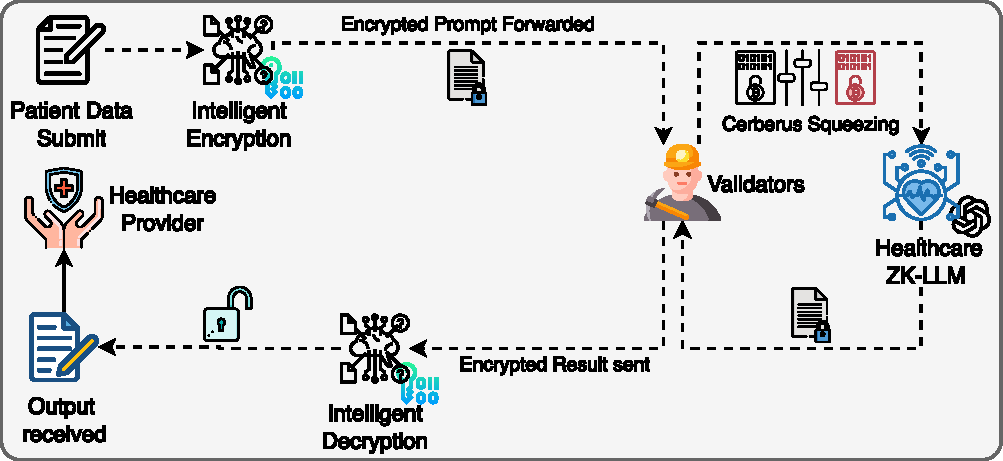
\includegraphics[width=\linewidth]{zk_llm_health.pdf}
\caption{Healthcare application scenario of BasedAI.}
\label{fig:zk_llm_health}
\end{figure}


\subsection{Threat Detection and Anomaly Monitoring}
The rapid growth of Web3 and AI applications has resulted in the creation of vast quantities of data, making it increasingly challenging to identify and flag anomalous patterns. In response, the integration of LLMs with blockchain has shown potential in the detection and mitigation of anomalous behavior. For instance, transformer and LLM-based models have been deployed to identify fraudulent activities in blockchain and DeFi environments~\cite{gai2023blockchain}. These approaches introduce data processing pipelines that include custom data encoding, domain-specific tokenization, and tree-structured intermediate trace representations. By utilizing unsupervised and self-supervised learning to model complex patterns within transaction traces, such systems enable real-time anomaly detection with high throughput. They also rank transactions based on log-likelihood scores to trigger defense mechanisms like smart contract pauses. Despite the promising results of these LLM-driven tools, their effectiveness remains highly dependent on detection thresholds and the scalability of token embeddings. Similarly, deep learning-based frameworks have been tailored for specific protocols (e.g., Olympus DAO\footnote{\url{https://www.olympusdao.finance/}}) to enhance anomaly detection~\cite{song2023anomaly}. By combining VAEs and transformers, these methods capture both short-term local information and long-term dependencies within on-chain data. Analyzing features such as token volume, transaction count, and active user numbers allows for the identification of malicious attacks and protocol changes. While this improves DeFi security, the applicability of such specific models is often limited to the protocols they were trained on.

Beyond transaction-centric analysis, recent research has focused on hybrid frameworks that address data privacy and structural complexity in distinct environments. To handle the specific resource constraints of the IoT sector, integrated frameworks combining blockchain, FL, and Split Learning (SL) have been proposed~\cite{batool2022block}. These solutions address data privacy and real-time detection challenges by employing transformer models to analyze temporal data from communication service providers within a decentralized paradigm. Such approaches demonstrate competitive performance, achieving accuracies around 86\%; however, scalability is often affected by increased resource consumption, communication overhead, and blockchain-related costs. Shifting focus to the structural integrity of DApps, heterogeneous graph transformer networks have been introduced to detect abnormal behaviors in smart contracts~\cite{liu2022blockchain}. By constructing heterogeneous information networks, these models capture the multi-relational structure of Ethereum and automate meta-path learning, which is critical for identifying anomalies without manual intervention. Experimental results indicate that graph-based transformers outperform traditional models like Support Vector Machines (SVM)~\cite{suthaharan2016support} and CNNs in terms of accuracy and stability. Nevertheless, their performance heavily relies on the quality and completeness of the underlying data, where incomplete or noisy inputs can significantly degrade detection accuracy.

\subsection{Data and Resource Management}
Data management solutions prioritize both security and scalability to address critical needs in areas such as healthcare and AI computation. By leveraging decentralized infrastructure, these solutions ensure data integrity, secure access control, and efficient distribution of computing resources to establish robust infrastructures for diverse applications. For example, Niranga et al.~\cite{niranga2022design} contribute to the development of secure, decentralized access control frameworks in healthcare for broader applications in Web3. The authors propose a blockchain-based system to enhance the security and management of medical data in hospitals. The object here is to address vulnerabilities highlighted by ransomware attacks during the COVID-19 pandemic. The study demonstrates a proof-of-concept implementation using the Remix IDE\footnote{\url{https://remix.ethereum.org/}} and Truffle Suite\footnote{\url{https://archive.trufflesuite.com/}}. This highlights the system's potential to decentralize access control and ensure data integrity. On the other hand, DeepBrain Chain (DBC)~\cite{web-dbc} emerges as a pioneering platform leveraging the convergence of blockchain, Web3, and DeAI to provide a decentralized, scalable, and cost-effective GPU computing network. By integrating blockchain, DBC ensures secure, transparent, and efficient sharing and trading of AI computing power, datasets, and models. This decentralized approach democratizes access to high-performance AI resources, reducing costs by up to 70\% compared to traditional cloud computing solutions. DBC supports various AI applications, including model training, decentralized AI applications, and AI-powered IoT networks. Its ecosystem also facilitates the creation and deployment of smart contracts, which enhances the functionality of decentralized AI and Web3 projects. Furthermore, DBC's GPU leasing and support for DAOs position it as a critical infrastructure provider in the Web3 landscape to drive advancements in AI, cloud gaming, and the metaverse.

\begin{table*}[!t]
\centering
\caption{Summary of application and use case scenarios.}
\label{tab:app}
\footnotesize
\selectfont
\setlength\tabcolsep{0.6pt}
\begin{tabularx}{\linewidth}{
>{\hsize=0.05\hsize}X
>{\hsize=0.11\hsize}Z
>{\hsize=0.08\hsize}Z
>{\hsize=0.14\hsize}Z
>{\hsize=0.14\hsize}Z
>{\hsize=0.14\hsize}Z
>{\hsize=0.10\hsize}Z
>{\hsize=0.22\hsize}Y}
\toprule 

\textbf{Ref.} & \textbf{Objective} & \textbf{Domain} & \textbf{Application} & \textbf{Integration} & \textbf{GenAI Model} & \textbf{Metrics} & \multicolumn{1}{c}{\textbf{Remarks}} \\\midrule

\cite{pearlson2024evaluating} & \makecell[c]{high-quality\\annotation} & DeFi & \makecell[c]{LLM-based \\NER} & \makecell[c]{LLMs with DeFi-\\specific data} & \makecell[c]{GPT-3.5; \\GPT-4; \\LLaMA-2-13b} & \makecell[c]{PR; RE; \\F1} & \makecell[l]{i) Limited zero-shot success;\\ii) Improved with fine-tuning;\\iii) Domain-specific innovation} \\\hline 

\cite{sun2024zkllm} & \makecell[c]{Verifiable LLM \\inference} & ZKP & \makecell[c]{Secure model\\verification} & ZKP for LLM & \makecell[c]{zkLLM; \\zkAttn} & \makecell[c]{Proof size;\\verification\\time} & \makecell[l]{i) Efficient CUDA support;\\ii) Handle large LLMs;\\iii) Protects model privacy} \\\hline 

\cite{wellington2024basedai} & \makecell[c]{Privacy \\computation} & ZKP & \makecell[c]{Encrypted model \\processing} & \makecell[c]{FHE with \\quantization} & ZK-LLM & \makecell[c]{Computation \\efficiency} & \makecell[l]{i) Enhanced data privacy;\\ii) Support multi-user tasks;} \\\hline 

\cite{gai2023blockchain} & \makecell[c]{Real-time \\transaction\\analysis} & AD & \makecell[c]{Intrusion \\detection on\\Ethereum} & \makecell[c]{LLM with \\transaction\\traces} & Transformer & \makecell[c]{PR; RE;\\F1} & \makecell[l]{i) Unsupervised learning;\\ii) Detect DeFi attacks;\\iii) High throughput} \\\hline 

\cite{song2023anomaly} & \makecell[c]{Detect\\transaction \\patterns} & AD & \makecell[c]{DAO-based\\analysis} & \makecell[c]{GenAI\\with DEX} & \makecell[c]{VAE; \\Transformer} & \makecell[c]{Anomaly \\score; \\frequency} & \makecell[l]{i) Capture short- and \\long-term patterns;\\ii) High computational cost} \\\hline 

\cite{batool2022block} & \makecell[c]{Computation\\offloading} & AD & \makecell[c]{IoT-based \\real-time\\analysis} & \makecell[c]{FL, SL with\\blockchain} & Transformer & \makecell[c]{PR; RE; \\F1} & \makecell[l]{i) Support resource-limited \\clients;\\ii) High training cost} \\\hline 

\cite{niranga2022design} & \makecell[c]{Access \\management} & DM & \makecell[c]{Medical data\\access control} & \makecell[c]{Smart contract,\\Web3 API} & N/A & \makecell[c]{Access\\control} & \makecell[l]{i) Immutable records;\\ii) Role-based access;} \\\hline 

\cite{la2023sonar} & \makecell[c]{NFT-based \\search queries} & SA & \makecell[c]{Multimodal\\NFT analysis} & \makecell[c]{Embed Image, \\text with Web3} & BERT; ViT & \makecell[c]{Network\\size} & \makecell[l]{i) Detect plagiarism risks;\\ii) Handle large data} \\\hline 

\cite{wahidur2024enhancing} & \makecell[c]{Improve\\zero-shot SA} & SA & \makecell[c]{Social media,\\crypto analysis} & \makecell[c]{Fine-tuned LLM \\with PE} & \makecell[c]{DistilBERT; \\MiniLM; \\FLAN-T5} & \makecell[c]{AC, PR, \\RE, F1} & \makecell[l]{i) Optimal instruction tuning;\\ii) Corpus size critical for\\performance} \\\bottomrule

\end{tabularx}
\begin{tablenotes}
\item \textbf{DEFI}=Decentralized Finance; \textbf{AC}=Accuracy; \textbf{PR}=Precision; \textbf{RE}=Recall; \textbf{F1}=F1-Score; \textbf{AD}=Anomaly Detection; \textbf{SL}=Split Learning; \textbf{DM}=Data Management; \textbf{N/A}=Not Available; \textbf{SA}=Sentiment Analysis; \textbf{PE}=Prompt Engineering.
\end{tablenotes}
\end{table*}


\subsection{User Behavior and Sentiment Analysis}
Sentiment analysis has become a crucial tool for understanding user behavior and market dynamics within digital ecosystems, particularly in sectors such as NFTs and cryptocurrency markets. For instance, SONAR~\cite{la2023sonar} is a web-based tool developed to explore the Web3-based NFT landscape. It utilizes pre-trained models such as BERT~\cite{devlin2018bert} and ViT~\cite{khan2022transformers} for text and images, respectively to produce multimodal embeddings for network analysis. These embeddings are used to construct directed, timestamped, weighted graphs, allowing users to examine NFTs at both the individual and collection levels. SONAR processes a dataset of 6.1 million transactions, but its use of pre-trained models does not fully capture the unique characteristics of NFTs. This limitation affects the accuracy of its representations. Additionally, the lack of minting time data limits the tool's ability to offer comprehensive insights into the NFT landscape. On the other hand, Wahidur et al.~\cite{wahidur2024enhancing} explore the intersection of zero-shot sentiment analysis and LLMs in the context of cryptocurrency markets. The effectiveness of supervised fine-tuning (SFT) and instruction tuning (IT) is investigated to enhance the performance of pre-trained LLMs on unseen tasks. The authors compare three LLMs: DistilBERT~\cite{sanh2019distilbert}, MiniLM~\cite{wang2020minilm}, and FLAN-T5~\cite{suresh2023semantic}. They show that models fine-tuned with instructions outperform those fine-tuned without instructions by an average of 16\%. They also demonstrate the superior performance of the larger model (e.g., FLAN-T5), which achieves an accuracy of 75.17\%. While larger models benefit more from instruction tuning, the resource-intensive nature of these models raises concerns about scalability, particularly in real-time or large-scale applications where computational efficiency is critical.

\begin{table*}[!t]
\centering
\caption{Summary of key challenges and future directions.}
\label{tab:future}
\footnotesize
\selectfont
\setlength\tabcolsep{0.6pt}
\begin{tabularx}
{\linewidth}{
>{\hsize=0.15\hsize}X
>{\hsize=0.20\hsize}X
>{\hsize=0.22\hsize}X
>{\hsize=0.20\hsize}X
>{\hsize=0.20\hsize}X
}\toprule

\textbf{Challenges} & \textbf{Overview} & \textbf{Key Techniques} & \textbf{Research Gap} & \textbf{Future Direction} \\\midrule

\makecell[l]{Scalability and\\Interoperability} & \makecell[l]{High computational \\demands for DeAI/GenAI;\\Limited cross-chain \\data-exchange} & \makecell[l]{LLM-based smart contracts;\\Off-Chain computations} & \makecell[l]{Lack of scalable \\cross-chain solutions} & \makecell[l]{Develop L2 solutions for\\GenAI/DeAI;\\Enhance cross-chain\\collaboration} \\\hline

\makecell[l]{Dataset \\Availability} & \makecell[l]{Limited blockchain-\\specific datasets;\\Privacy concerns on\\data aggregation} & \makecell[l]{Synthetic data\\ (GANs,VAEs);\\Decentralized data \\exchanges} & \makecell[l]{Lack of standardized \\and privacy-compliant\\data} & \makecell[l]{ Standardize formats;\\Incentivize high-quality\\data sharing} \\\hline

\makecell[l]{Interpretability\\and Explainability} & \makecell[l]{Opacity in large models;\\Accountability challenges \\in decentralized settings} & \makecell[l]{Attention mechanisms;\\Model pruning} & \makecell[l]{Limited transparency \\in critical applications} & \makecell[l]{Develop lightweight\\interpretable models} \\\hline

\makecell[l]{Interdisciplary\\ Research and \\Sustainability} & \makecell[l]{Integration challenges for \\supply chain management} & \makecell[l]{Blockchain, smart\\ contracts; Digital Twin, RL} & \makecell[l]{Synchronization issues \\in decentralized contexts} & \makecell[l]{Explore interdisciplinary \\approaches for \\sustainable supply chains} \\\hline

\makecell[l]{Quantum \\Computing} & \makecell[l]{Quantum threats to \\cryptographic methods} & \makecell[l]{Quantum key distribution;\\Post-quantum cryptography} & \makecell[l]{Vulnerabilities in current\\cryptographic protocols} & \makecell[l]{Research quantum-resistant\\protocols;\\Integrate quantum-safe\\ cryptography} \\\hline

\makecell[l]{Ethical and Social\\Implication} & \makecell[l]{Power concentration in \\decentralized networks;\\Misinformation risks \\with GenAI} & \makecell[l]{Fair influence distribution;\\Misinformation detection} & \makecell[l]{Lack of fair influence \\mechanisms;\\Safe GenAI guidelines} & \makecell[l]{Ensure fair influence;\\Mitigate misinformation} \\\bottomrule

\end{tabularx}
\end{table*}


	
\section{Research Challenges and Future Directions} \label{sec:future}
The trust-to-augmentation framework presents both significant opportunities and structural constraints for decentralized intelligence systems. The analysis in Sections~\ref{sec:blockchain}--\ref{sec:genai} and existing surveys on decentralized AI, Web3 middleware, and generative architectures~\cite{xu2024survey,savadatti2025survey,choi2025technological,luo2024survey,javadpour2024decentralized,wang2024sok} show that many deployed or prototype systems already combine blockchain, Web3, DeAI, and GenAI components. However, these efforts often remain fragmented and seldom implement the full four-layer architecture in a coherent and verifiable way. This section synthesizes these gaps as open challenges for implementing the framework in real-world settings and outlines future directions that directly extend the surveyed literature. A concise summary of the challenge themes and corresponding directions appears in Table~\ref{tab:future}.

\subsection{Cross-layer Implementation Gaps}
The framework in Section~\ref{sec:framework} structures decentralized intelligence into four interdependent layers grounded in verifiable execution, privacy under transparency, and coordinated autonomy~\cite{xu2024survey,savadatti2025survey,wang2024sok}. Subsequent sections map representative systems to these layers, including TEEs and rollups in the trust-based execution layer, interoperability protocols and privacy middleware~\cite{huang2023overview,wan2024web3}, collaborative learning meshes~\cite{luo2024survey,javadpour2024decentralized}, and GenAI-driven user interfaces and agents~\cite{huang2024large}. Individual designs often deliver strong properties at one or two layers, but current systems rarely expose stable interfaces that support robust composition of all four layers~\cite{liu2024blockchainempowered}. Several cross-layer gaps emerge from this survey and from the integration challenges identified in Section~\ref{sec:framework}. A first gap concerns canonical interfaces and invariants. Existing systems seldom define clear contracts that specify what lower layers guarantee to higher layers in terms of consistency, latency, and security, and what higher layers commit to preserve when invoking lower-layer services~\cite{wan2024web3}. A second gap concerns end-to-end performance and reliability models. Performance analysis typically focuses on blockchain throughput or model accuracy, yet joint models that link transaction ordering, off-chain computation, and agent decision latency remain underdeveloped. A third gap concerns identity, reputation, and incentive alignment across layers, where learning systems and GenAI agents frequently maintain local reputation or policy state that does not align with long-lived identities and incentives on-chain~\cite{dorri2018multi}. A final gap relates to reference implementations and shared testbeds, since the community has many isolated prototypes but few deployments that exercise all four layers under realistic adversarial and regulatory conditions.

Future work on the framework benefits from explicit interface definitions, cross-layer protocols, and open reference stacks. Research that specifies machine-readable contracts between layers, along with formal guarantees and monitoring hooks, enables independent evolution of each layer without loss of global safety. Cross-layer performance models that couple on-chain and off-chain computation create a basis for systematic optimization and capacity planning~\cite{xu2024survey}. Shared experimental platforms that expose realistic transaction traces, agent behaviors, and governance events allow comparative evaluation of new designs and support replication of complex experiments, particularly when they incorporate the multi-domain scenarios discussed in Section~\ref{sec:app}.

\subsection{Scalability and Interoperability across Layers}
Scalability and interoperability remain foundational challenges for decentralized intelligence. The trust-based execution and middleware layers integrate mechanisms such as sharding, sidechains, rollups, and cross-chain bridges to increase throughput and reduce transaction costs~\cite{wan2024web3,alsagheer2023decentralized}. Collaborative learning meshes distribute training and inference across devices and edge infrastructure~\cite{luo2024survey,javadpour2024decentralized}, and GenAI components introduce computationally intensive inference and content generation~\cite{huang2024large}. The surveyed systems show that these techniques improve performance at individual layers, but they do not yet provide consistent guarantees when applications span chains, learning meshes, and generative agents.

Scalability gaps appear when resource allocation decisions ignore dependencies across layers. Many systems treat blockchain throughput, model training capacity, and GenAI inference load as separate engineering problems, which leads to local optimizations that degrade end-to-end latency or reliability. Interoperability gaps arise because chains, rollups, and FL fabrics often expose incompatible data models, security assumptions, and failure semantics~\cite{wan2024web3}. GenAI agents frequently depend on off-chain state and cross-chain liquidity without robust guarantees about the freshness, completeness, or finality of the underlying data. These gaps translate into brittle applications that behave unpredictably under load spikes, network partitions, or adversarial manipulation. Joint resource orchestration and cross-layer communication standards form a central direction for future work. Multi-layer schedulers and cryptoeconomic mechanisms that allocate compute, bandwidth, and storage across chains, learning meshes, and inference services can provide predictable application performance under cost and energy constraints. Standardized interfaces that export succinct, verifiable summaries of on-chain and off-chain state give collaborative learning systems and GenAI agents stable views of the environment. 

\subsection{Data Availability, Quality, and Evaluation Benchmarks}
Data availability and evaluation practices determine the reliability and generality of decentralized intelligence systems. Blockchain ecosystems expose transparent transaction records, asset movements, and smart contract events, but these traces rarely include human context, socio-economic attributes, or explicit labels for complex behaviors such as collusion and manipulation~\cite{jain2024wire}. DeAI and GenAI components require longitudinal, cross-modal datasets that connect on-chain activity with off-chain actions, natural language descriptions, and governance outcomes~\cite{akanfe2024blockchain,nikolentzos2023synthetic}. The survey reveals early efforts to construct such datasets and benchmarks, yet current resources remain narrow in scope and fragmented across projects.

Gaps in dataset construction and evaluation hinder robust deployment. Public datasets for decentralized intelligence often lack coverage for minority behaviors and underrepresented user groups, which introduces systemic bias in downstream models~\cite{liu2019decentralized}. Labels for security-relevant phenomena such as value extraction, governance attacks, and coordinated market manipulation frequently appear in isolated case studies rather than reusable corpora. Datasets that couple agent behaviors, communication patterns, and governance events are rare, which limits the community's ability to evaluate collective dynamics and emergent risks. Evaluation benchmarks frequently target either model accuracy or on-chain efficiency and seldom combine trust, privacy, fairness, and economic stability metrics in a single suite. Future work can prioritize open, multi-modal datasets and shared benchmarks that reflect the four-layer architecture. Curated corpora that integrate transaction traces, textual artifacts, governance decisions, and agent actions would support training and evaluation of DeAI and GenAI systems that operate in Web3 environments. Dataset construction processes require systematic methods for bias detection and documentation, along with incentive mechanisms that reward contributors who supply high-quality, diverse data under clear privacy guarantees. 

\subsection{Model Robustness, Interpretability, and Verification}
Robust and interpretable models are essential for decentralized intelligence because decisions often carry direct financial, legal, or governance consequences. Surveyed systems explore attention mechanisms, causal graphs, symbolic constraints, and rule extraction to explain DeAI and GenAI outputs~\cite{huang2024large}, and some works log explanations or decision traces on-chain to support auditing~\cite{costa2023show,niu2021review}. However, interpretability mechanisms usually appear as auxiliary modules rather than primary design constraints, and many architectures provide no guarantees that explanations remain faithful when the environment or adversarial conditions change~\cite{cheng2024survey,dwivedi2023explainable}. Robustness gaps manifest when models face attacks such as data poisoning, adversarial prompts, and colluding agents~\cite{luo2024survey,javadpour2024decentralized}. Collaborative learning meshes often assume honest majority behavior and benign data sources, even though adversaries can influence gradients, labels, or prompts to manipulate downstream decisions. GenAI agents that propose transactions or governance actions can introduce subtle, hard-to-detect harms when trained on biased or strategically curated data~\cite{kim2024large}. Verification gaps arise because on-chain records typically log decisions and outcomes but do not encode evidence that a decision followed a specified policy or constraint set. As a result, users and regulators struggle to assess whether autonomous behaviors respect contractual, regulatory, or ethical requirements.

Research on robustness, interpretability, and verification can move toward mechanisms that integrate cryptographic guarantees with model-level analysis. Verifiable computing techniques, ZKPs, and succinct attestations for model execution can anchor off-chain inference and learning in on-chain evidence~\cite{huang2023overview}. Policy-aware architectures that log machine-readable rationales and constraint checks alongside actions increase trust in autonomous behaviors and support independent auditing. Evaluation methodologies that test systems under adversarial data, prompt perturbations, and colluding agents, and that simultaneously measure explanation fidelity and impact on affected users, would provide a more complete view of system reliability.

\begin{figure}[!t]
\centering
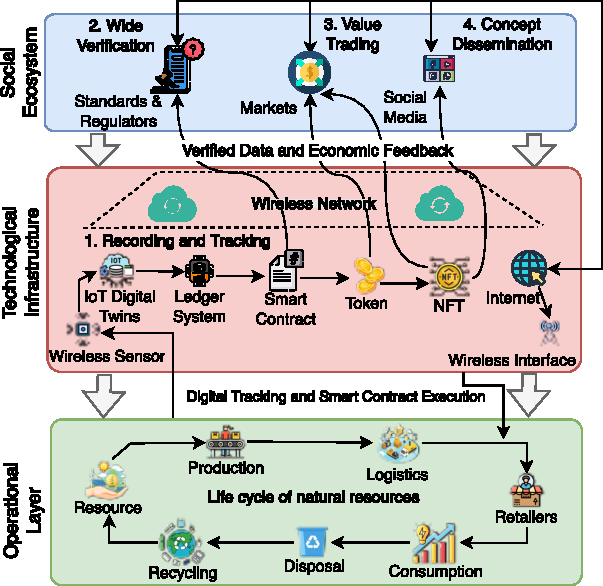
\includegraphics[width=\linewidth]{sustain.pdf}
\caption{Blockchain-based sustainable supply chain.}
\label{fig:sustain}
\end{figure}

\subsection{Sustainable and Interdisciplinary Design for Real-world Systems}
Decentralized intelligence intersects with domains such as finance, supply chains, energy, mobility, and healthcare, where environmental impact, regulatory alignment, and social outcomes matter as much as technical performance~\cite{wang2024traceability}. Figure~\ref{fig:sustain} illustrates one example in the supply chain context, where blockchain records provenance and logistics information and AI components analyze risk, compliance, and sustainability indicators. The surveyed case studies demonstrate potential for improved transparency and coordination, yet few works report complete life-cycle assessments or rigorous evaluations of environmental and social effects~\cite{liu2024blockchainempowered}.Several gaps limit progress toward sustainable and interdisciplinary design. Many proposals focus on technical feasibility and immediate efficiency gains but do not quantify long-term energy consumption, hardware turnover, or induced demand from new applications~\cite{naraganahalli2025decentralized}. Domain experts in law, economics, public policy, and social sciences often participate only at late stages of system design, which leads to misalignment between technical mechanisms and institutional realities. Empirical studies that track how decentralized intelligence systems reshape labor relations, market structures, and public service provision remain scarce, especially outside finance.

Co-designed pilots with stakeholders in critical infrastructures and public institutions form a key direction. Projects that align cryptoeconomic incentives with environmental and social objectives require models that internalize externalities in tokenomics, fee structures, and validator rewards. Interdisciplinary methodologies that combine qualitative fieldwork, formal modelling, and quantitative evaluation can reveal unintended consequences and support corrective governance~\cite{naraganahalli2025decentralized}. Open reporting of operational metrics, incident data, and sustainability indicators would enable evidence-based debate about the role of decentralized intelligence in long-term socio-technical transitions.

\begin{figure*}[!t]
\centering
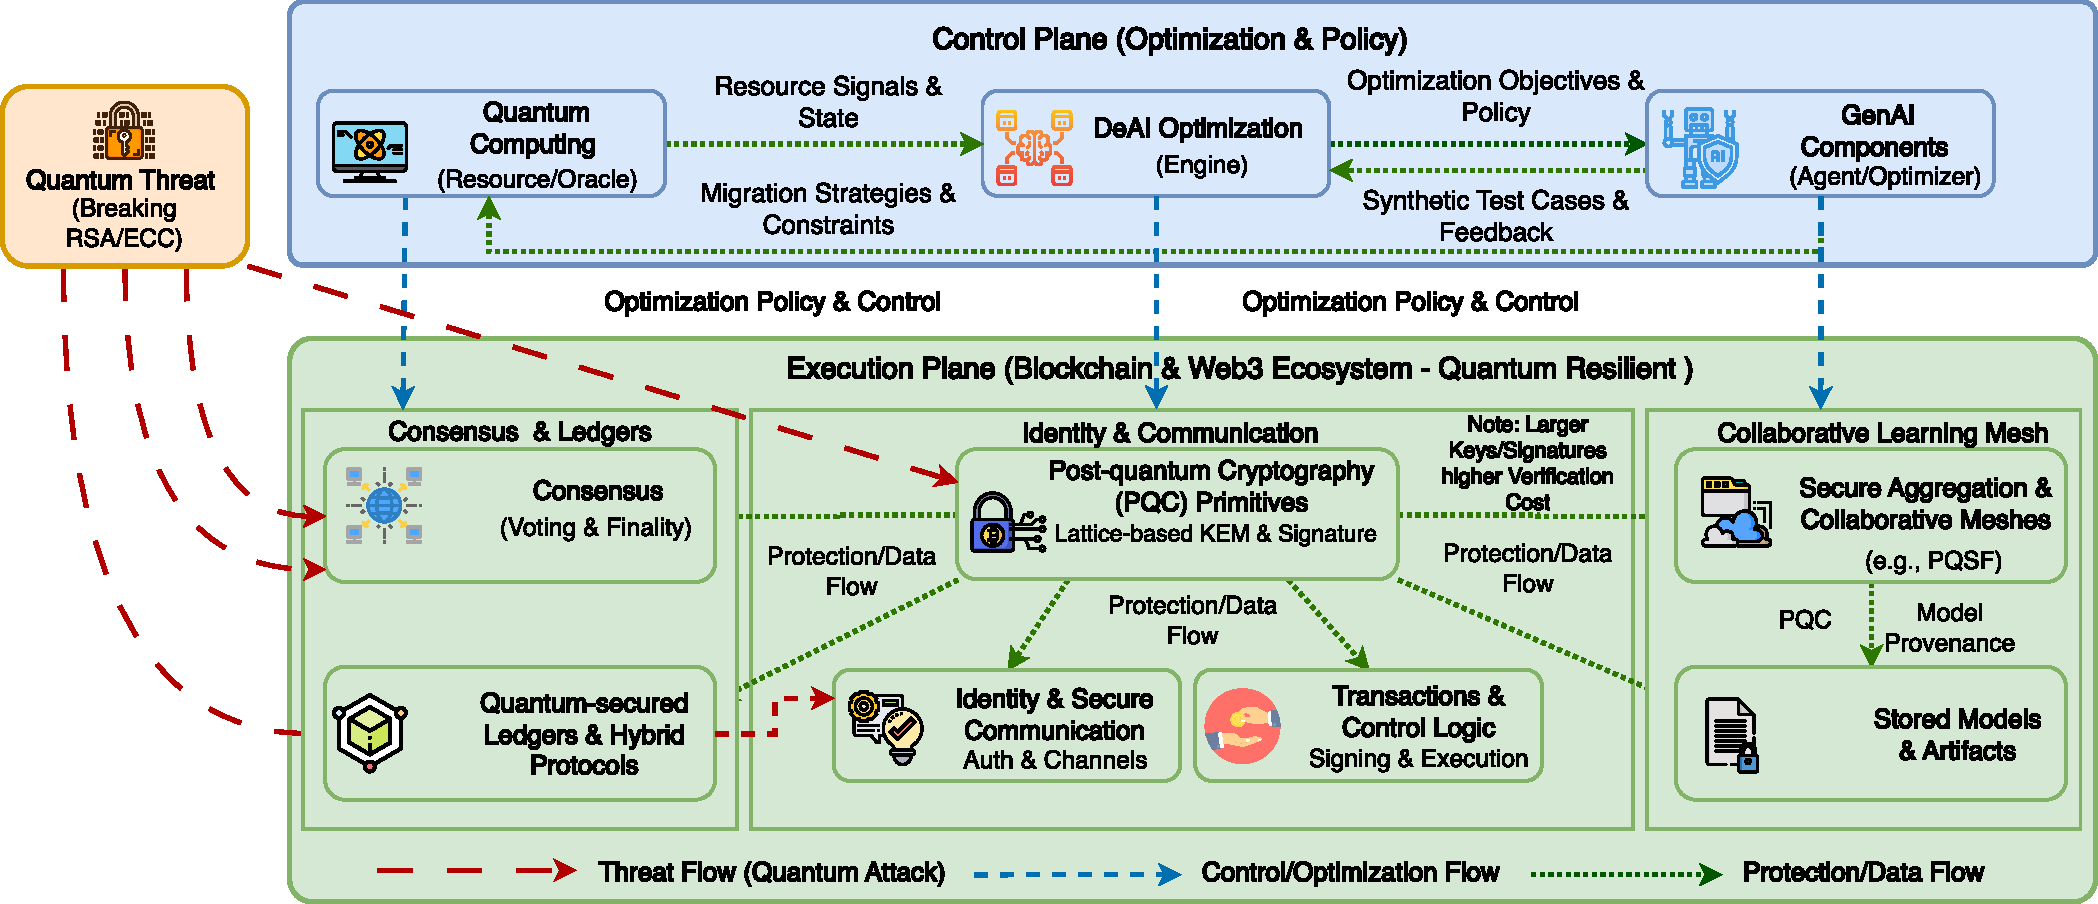
\includegraphics[width=0.90\linewidth]{quantum-v2.pdf}
\caption{GenAI-driven quantum blockchain framework.}
\label{fig:quantum}
\end{figure*}

\subsection{Quantum-resilient Decentralized Intelligence}
Quantum computing poses a direct threat to the public key cryptography that underlies blockchain consensus, identity management, and secure communication~\cite{ren2025building,mehic2020quantum}. Blockchain, Web3, and FL systems rely on RSA and elliptic-curve signatures for transaction validation and control logic~\cite{xu2023quantum}. Large-scale quantum computers break these cryptographic fundamentals~\cite{ricci2024hybrid}. This enables forged signatures, ledger manipulation, and impersonation of long-lived identities if timely migration is not achieved~\cite{gharavi2024post,khodaiemehr2023navigating}. Post-quantum cryptography (PQC) offers candidates that remain secure against classical and quantum adversaries, including lattice-based key-encapsulation and signature schemes~\cite{gharavi2024post,sikeridis2020assessing}. For blockchain, recent work proposes quantum-secured ledgers and hybrid protocols that combine existing consensus with post-quantum primitives~\cite{reddy2025quantum}. In FL and collaborative meshes, frameworks such as PQSF integrate lattice-based encryption into secure aggregation, and other designs use post-quantum tools to protect communication and stored models~\cite{zhang2024pqsf,umer2025quantum}. Post-quantum signatures secure model artifacts and update histories for long-term provenance~\cite{castiglione2025enhancing}, although these schemes typically increase key sizes, signature sizes, and computational overhead~\cite{gharavi2024post,vishwakarma2024qiskit}. Figure~\ref{fig:quantum} depicts a two-plane GenAI-driven quantum blockchain framework. The control plane combines quantum computing resources, DeAI optimization, and GenAI agents to derive optimization objectives, policies, and migration constraints. These controls guide a quantum-resilient execution plane that integrates PQC to protect consensus, identity and communication, and transaction control logic. The framework also secures collaborative learning via PQC-enabled aggregation and model provenance across stored models and artifacts, while the threat flow highlights attack paths triggered by broken RSA and ECC.

Quantum-resilient decentralized intelligence requires end-to-end architectures and realistic migration strategies. Hybrid designs integrate classical and post-quantum signatures during the transition phase. This approach supports gradual key rollover for existing addresses and identities and provides a practical migration path. Such designs rely on joint-signature policies for validators and smart-contract accounts, as well as hybrid key exchange mechanisms in FL channels~\cite{khodaiemehr2023navigating,zhang2024pqsf,umer2025quantum}. If identity or consensus signatures remain vulnerable, adversaries impersonate model owners, forge inference and provenance proofs, and compromise the long-term auditability of training and governance~\cite{khodaiemehr2023navigating,castiglione2025enhancing}. As a result, quantum readiness and post-quantum migration emerge as cross-cutting design objectives for next-generation decentralized intelligence platforms.


\subsection{Governance, Ethics, and Human Oversight}
Governance and ethics form a critical dimension of decentralized intelligence because systems coordinate resources, rights, and responsibilities across many stakeholders. The survey covers decentralized autonomous organizations, protocol governance councils, and data governance structures that define how updates, parameter changes, and access decisions occur~\cite{dorri2018multi,wang2024sok}. GenAI agents now participate in these processes as decision support tools, autonomous proposal generators, or even voting entities in experimental settings~\cite{naraganahalli2025decentralized}. Ethical questions arise around bias, misinformation, surveillance, and concentration of power in the hands of a few protocol maintainers or model providers. Current approaches reveal significant gaps in accountability and human oversight~\cite{saleem2025responsible,tabassum2025generative}. Many governance mechanisms rely on token-weighted voting, which can amplify wealth concentration and enable capture by large holders or coordinated colluding groups. Decision logs and discussions often live on external platforms that do not link cleanly to on-chain actions, which complicates auditing and accountability~\cite{chen2023can}. Technical work on fairness, privacy, and safety in AI rarely aligns with concrete governance procedures in Web3 ecosystems, and regulatory frameworks for AI and digital assets evolve in separate communities~\cite{naraganahalli2025decentralized}.

Governance and ethics research can advance mechanisms that align technical guarantees with institutional accountability. Protocols that embed verifiable audit trails, structured deliberation records, and explicit recourse mechanisms into on-chain governance provide stronger foundations for responsible autonomy~\cite{wang2024sok}. Cross-disciplinary studies that integrate legal analysis, political theory, and human-computer interaction can guide the design of voting schemes, delegation models, and participation incentives that mitigate capture and exclusion. Tooling for continuous monitoring, red teaming, and impact assessment of GenAI agents in decentralized infrastructures would support regulators, users, and communities that seek to maintain human oversight without sacrificing decentralization~\cite{naraganahalli2025decentralized}.

\subsection{Integrative Research Roadmap}
The research gaps and challenges in this section define a roadmap for decentralized intelligence that extends beyond isolated technical innovations. The trust-to-augmentation framework identifies how trust-based execution, privacy-preserving interoperable middleware, collaborative learning meshes, and generative augmentation depend on one another~\cite{xu2024survey,huang2023overview,luo2024survey,huang2024large}. The survey reveals that current systems address important parts of this architecture but rarely implement it as a cohesive whole. Cross-layer interfaces, data and evaluation infrastructures, robust and interpretable models, sustainable deployments, quantum resilience, and accountable governance are all essential to realize the framework in practice. Future progress depends on coordinated work across several cross-cutting themes. Architectural research needs shared abstractions, interface definitions, and reference implementations that link the four layers under clear guarantees. Data and benchmark initiatives need to treat on-chain, off-chain, and human-centric information as a combined design space for decentralized intelligence rather than as independent silos~\cite{jain2024wire}. Security and robustness research must integrate cryptographic, systems, and learning-theoretic insights to handle adversarial behavior at scale. Governance and ethics research must translate normative principles into concrete institutional and protocol designs~\cite{naraganahalli2025decentralized}.

\section{Conclusion} \label{sec:end}
This survey systematically integrates generative intelligence with decentralized protocols to articulate the foundational principles of decentralized intelligence. It introduces the trust-to-augmentation framework as an architectural stack in which trust-based execution underpins privacy-preserving middleware, a collaborative learning mesh coordinates secure workflows, and generative augmentation supports user-centric governance. The analysis indicates that effective integration can produce emergent properties that extend beyond individual components, allowing intelligence to propagate across the stack and enabling self-improving systems that reconcile enterprise-grade performance with decentralization. Advancing this field requires a shift from isolated optimizations toward holistic architectural innovation. Ongoing research must address persistent implementation gaps in cross-layer resource orchestration, quantum-resilient cryptographic migration, and verifiable evidence standards for off-chain AI decisions. A central open challenge remains defining canonical interfaces and shared economic models that allow these layers to operate collectively as a unified and trustless execution environment.

Realizing such an architecture in practice requires systematic mechanisms for evaluation, coordination, and governance across layers. Accordingly, the research community should prioritize integrated evaluation infrastructures capable of stress-testing consensus throughput, privacy guarantees, and agentic reasoning under a shared adversary model. Benchmarking standards must extend beyond conventional performance metrics to assess equitable influence, algorithmic accountability, and long-horizon economic stability in mixed human-agent ecosystems. Progress further depends on moving beyond static smart contracts toward autonomous economic agents with explicit capabilities for reasoning, adaptation, and self-governance under defined policy constraints. Such systems require externally verifiable action traces, principled recourse mechanisms, and durable oversight interfaces to ensure that user sovereignty is maintained under operational conditions. Finally, treating the trust-to-augmentation framework as an implementation blueprint provides a structured perspective for researchers and practitioners examining decentralized intelligence. This perspective informs the design of systems that aim for mainstream utility while preserving user sovereignty and ethical alignment.


\section*{Acknowledgments}
This work is supported by the National Key Research and Development Program of China (No. 2020YFA0909100) and the Basic and Applied Basic Research Foundation of Guangdong Province (No. 2023TQ07A264).

\biboptions{sort&compress}
\bibliographystyle{elsarticle-num}
\bibliography{REF_COSREV-D-25-00744-R1} 
\end{document}